\documentclass[14pt,CJKutf8,mathserif]{beamer}
\usepackage{CJKutf8,CJKnumb}
\usepackage{amsmath,amssymb,amsthm,amscd}
%\usepackage{asymptote}
\usepackage{wasysym}
\usepackage{gensymb}
\usepackage{enumitem}
\usepackage{tikz}
\usepackage{circuitikz}
\usepackage{epstopdf}
\usepackage[utf8]{inputenc}
\usepackage{manfnt}
\usetikzlibrary{positioning,calc}
\usetikzlibrary{shapes,snakes}
\tikzset{
>=stealth,
nonterminal/.style={rectangle,minimum size=6mm,draw=black,font=\ttfamily},
circleterminal/.style={circle,minimum size=1mm,draw=black},
circlenode/.style={circle,inner sep =0pt,minimum size=3pt,draw=black,fill=black},
noshapenode/.style={circle,inner sep =0pt,minimum size=0pt}
}
\mode<presentation>
{
  \usetheme{PaloAlto}
}
%\includeonlylecture{yinlun}
%\includeonly{content/chapter2-1}
%\includeonly{content/chapter2-2}
%\includeonly{content/chapter2-3}
%\includeonlylecture{wulimoxing}
\begin{document}

\begin{CJK}{UTF8}{song}
\title{计算机控制原理与应用}
\author{金波 \inst{1}}
\institute[西藏职业技术学院]{
\inst{1}
教务处\\ 西藏职业技术学院 }
\date{\today}
\begin{frame}
\titlepage
\end{frame}
\begin{frame}[allowframebreaks]{主要内容}
  \tableofcontents
\end{frame}
\chapter{平面图样绘制}
{\bfseries 知识目标}
\begin{itemize}
\item 了解国家制图标准和电气 AutoCAD 制图规范
\item 掌握平面图样的绘制步骤和方法
\item 掌握用 AutoCAD 绘制平面图样的基本步骤和方法
\item 掌握 AutoCAD 基本的绘图命令
\end{itemize}

{\bfseries 技能目标}
\begin{itemize}
\item 具备平面样抄绘能力
\item 具备使用AutoCAD绘制中等复杂程度的图样的能力
\item 具备阅读和分析平面图样的能力
\end{itemize}

{\bfseries 本章导引}

图\ref{fig:shangmu1}所示图纸即为图样,是根据投影法,并按照国家或国际标准的规定绘制的,用于工程施工或产品制造等用途的图。标准则是为了在一定范围内获得最佳秩序,而对活动或其结果规定共同的和重复使用的规则、导则或特性的文件。本章旨在通过讲解图\ref{fig:shangmu1}所示项目,使学生在完成项目的同时,了解和掌握国家制图标准中图幅、比例、线型、文字、标注等相关知识,以及通过AutoCAD进行图样绘制的步骤、方法、技巧和规范,并能运用所学的技巧和知识解决绘图过程中的实际问题,具备遵照国家制图标准和规范抄绘图样的能力。
\noindent
\begin{landscape}
\begin{figure}[htbp]
\centering
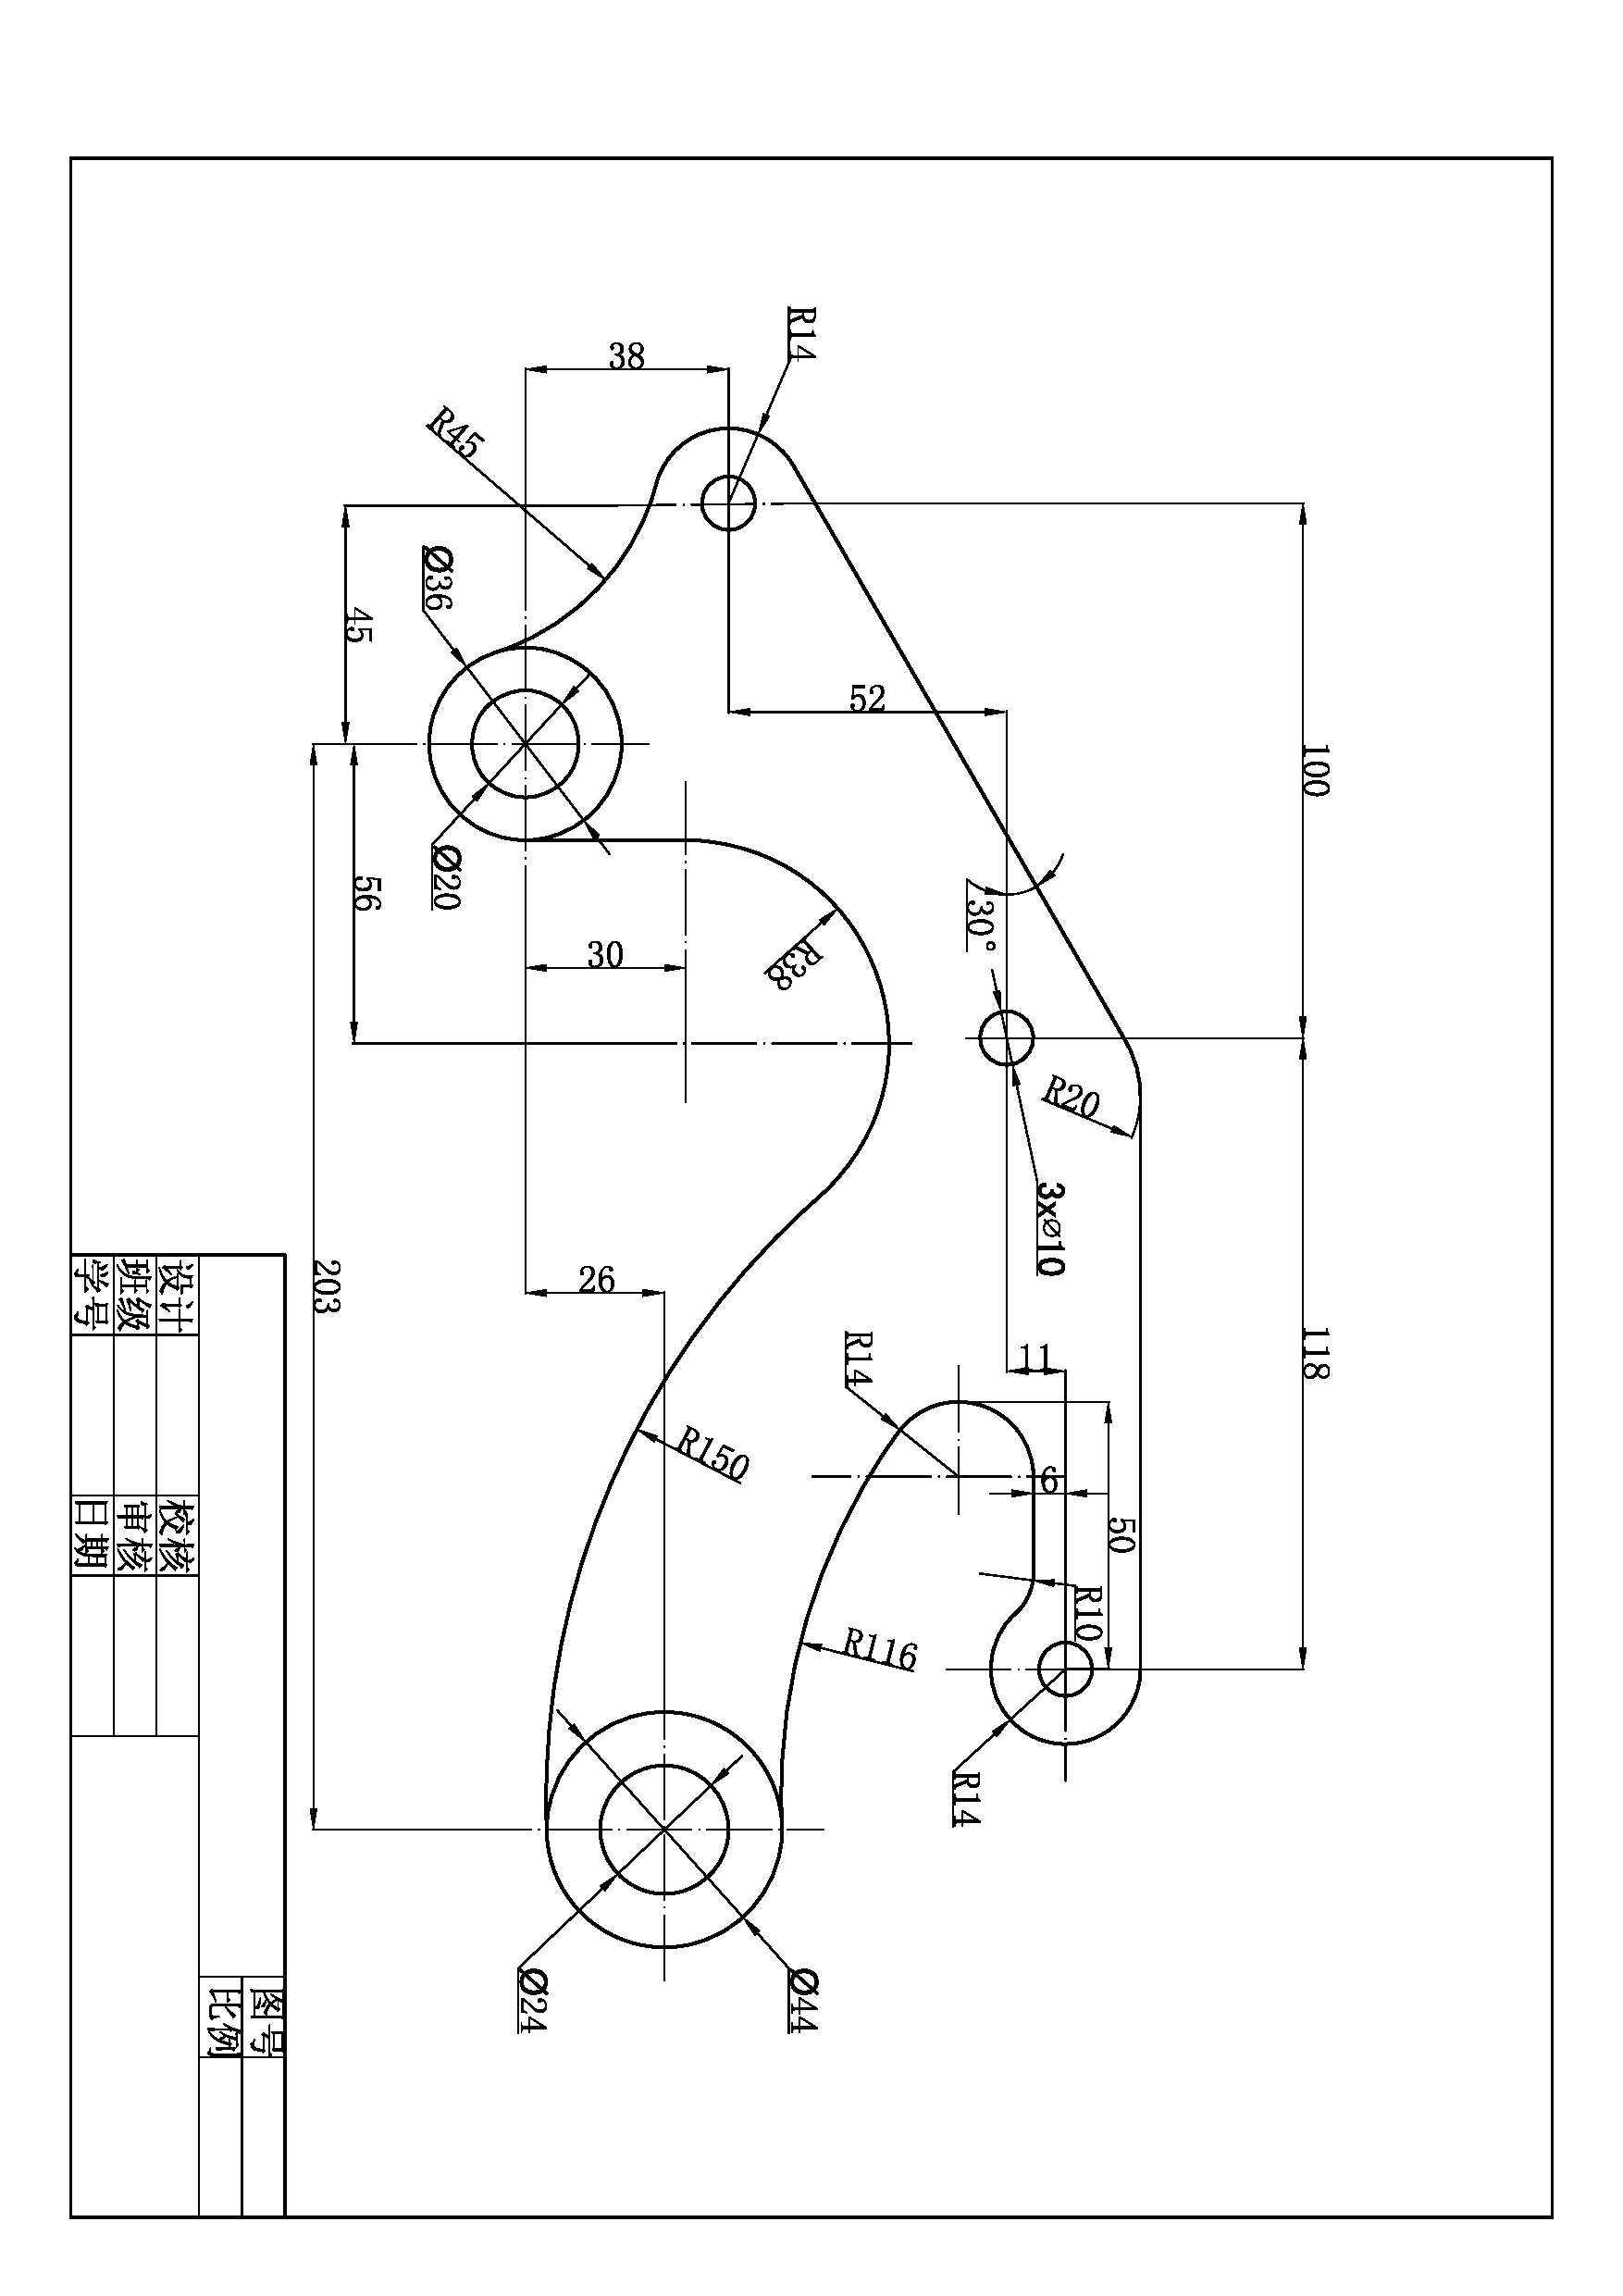
\includegraphics[scale=0.45,angle=90]{shu1.pdf}
\caption{项目一示例}\label{fig:shangmu1}
\end{figure}
\end{landscape}
\indent
%\newpage

\section{平面几何图(一)}\label{sec:gongzhi}

{\bfseries 知识目标}
\begin{itemize}
\item 掌握绝对坐标、相对坐标和极轴坐标的概念
\item 掌握limits命令的使用方法
\item 掌握point、line命令的使用方法
\item 了解国家制图标准中图幅的标准及与limits命令之间的关系
\end{itemize}

{\bfseries 技能目标}
\begin{itemize}
\item 能够完成工字图样的绘制
\end{itemize}

本任务以绘制图\ref{fig:shangmu1-1}所示的工字图样为目标,主要是为了帮助读者掌握Auto\-CAD 图形绘制过程中最重要的概念---坐标。坐标是AutoCAD精确绘的基础,对图形对象的精确定位起至关重要的作用。通过完成该任务来理解AutoCAD中图形的关键点的坐标描述方法,以及各种坐标表述方式的应用情景。其次是为了让读者掌握line命令的基本用法。
\enlargethispage{10pt}
\noindent
\begin{figure}[htbp]
\centering
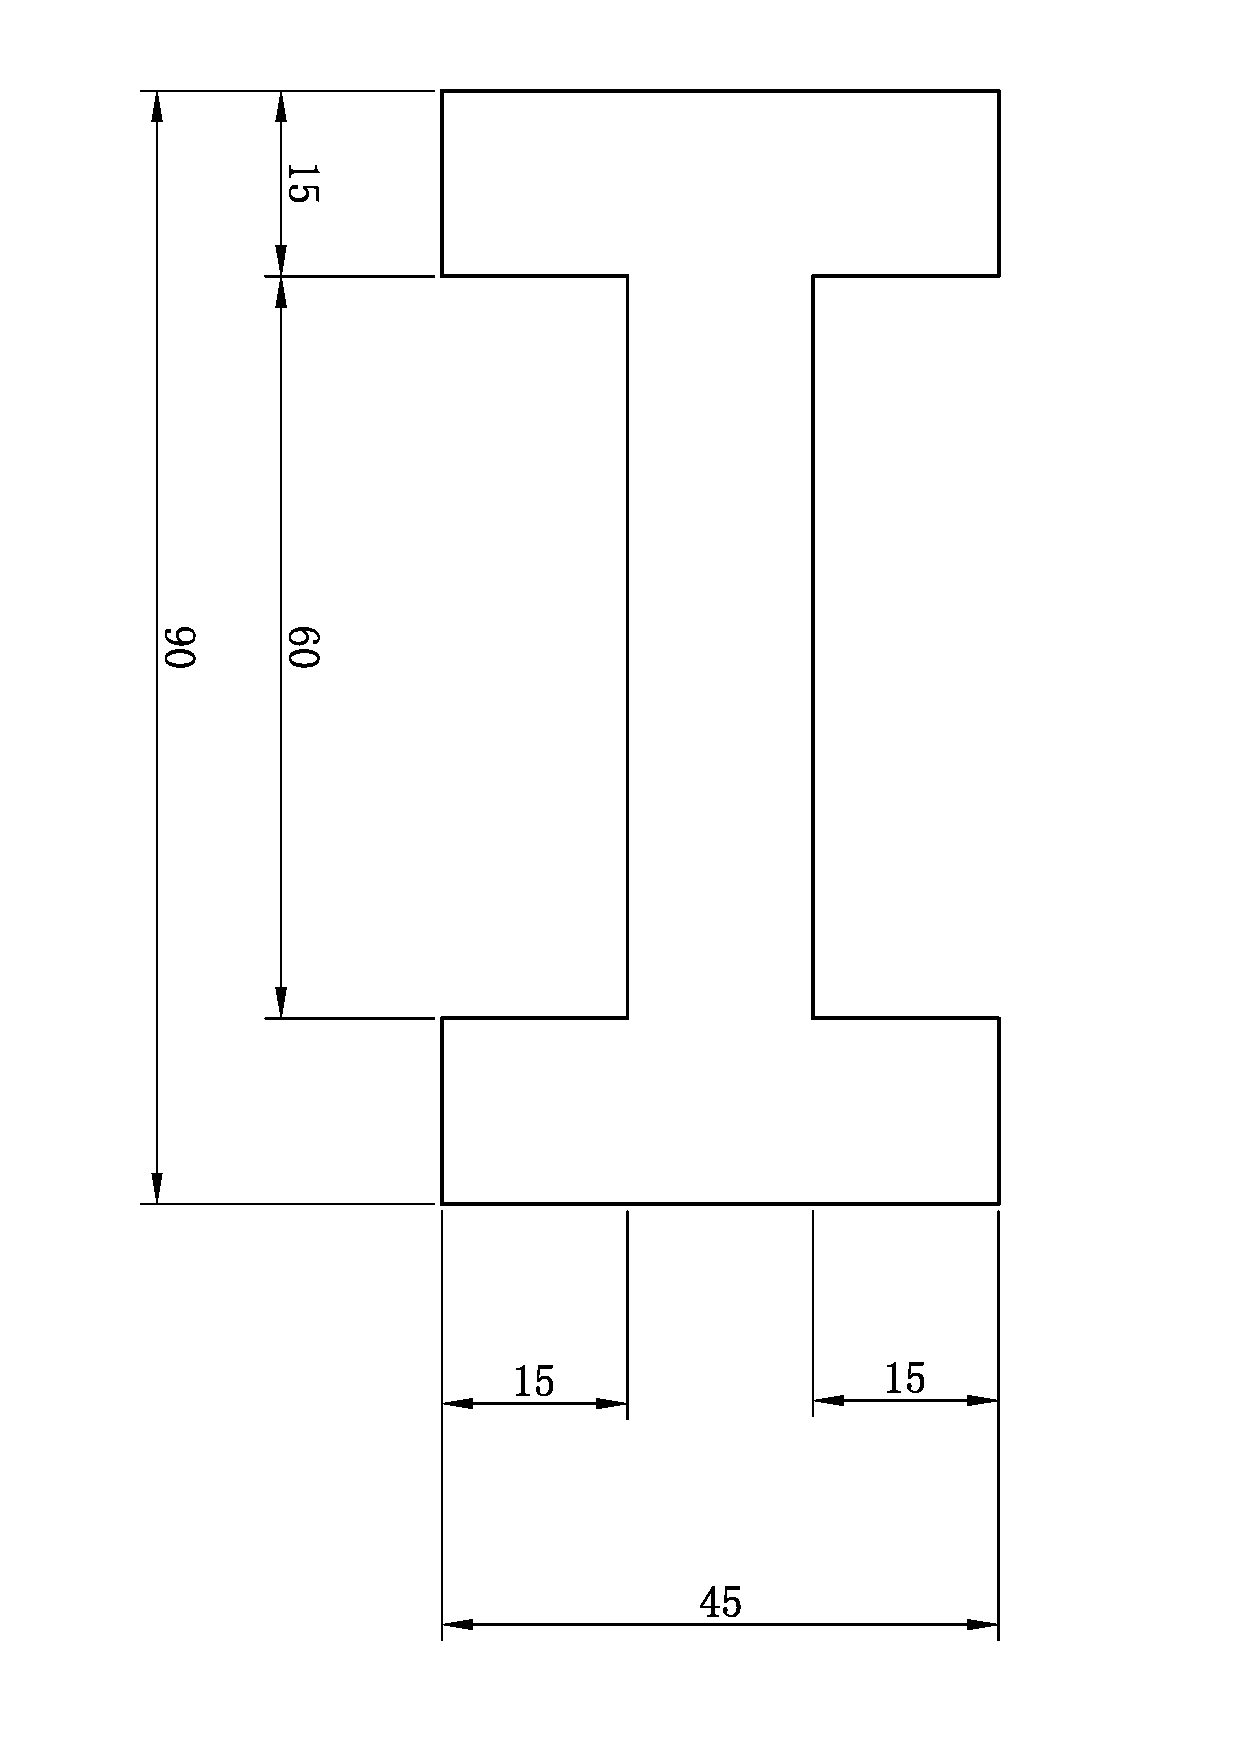
\includegraphics[scale=0.4,angle=90]{gongzi.pdf}
\caption{工字图样}\label{fig:shangmu1-1}
\end{figure}
\indent

\subsection{绘制图样}
\subsubsection{设置图形界限LIMITS}
AutoCAD中的绘图区域是无限大的,可以在绘图区的任何地方绘图。为一方便打印,一般需要设置一个绘图区域用来限制绘图的区域,不至于将图形绘制来区域之外。要实现此功能,用户使用“图形界限”命令进行设置。

在命令提示区输入limits 以执行“图形界限”命令。
\noindent
命令:  LIMITS\\
重新设置模型空间界限:\\
指定左下角点或 [开(ON)/关(OFF)] $<$0.0000,0.0000$>$:\\
指定右上角点 $<$420.0000,297.0000$>$: 297,210\\
\indent
LIMITS命令中【开(ON)】表示打开界限检查,此时不能够在图形界限以外输入点来创建图形对象。【关(OFF)】表示关闭界限检查,此时能够在图形界限以外输入图形对象。

\subsubsection{图形缩放显示ZOOM}
由于图\ref{fig:shangmu1-1}的尺寸比较小,为了便于观察绘图结果,我们需要先使用ZOOM命令先将图形显示区域缩放到图形界限范围。

\noindent
命令: ZOOM\\
指定窗口的角点,输入比例因子 (nX 或 nXP),或者
[全部(A)/中心(C)/动态(D)/范围(E)/上一个(P)/比例(S)/窗口(W)/对象(O)] $<$实时$>$: a
\indent

ZOOM命令中各个选项的含义如下:
\begin{itemize}
\item 全部(A):在平面图形中,缩放到整个图形界限
\item 中心(C):缩放显示由中心点和缩放比例(或高度)所定义的窗口
\item 动态(D):执行此选项,会出现一个视图框,通过调整视图框的大小,调整显示图形的大小
\item 范围(E):最大限度的显示所有图形
\item 上一个(P):回到上一次缩放
\item 比例(s):按输入比例值进行缩放
\item 窗口(W):最大限度地显示框选的图形
\item 对象(O):最大限度地显示选择的对象
\end{itemize}
\subsubsection{绘制图形}
绘制图\ref{fig:shangmu1-1}需要使用AutoCAD中的line命令。

\noindent
命令: line 指定第一点: 0,0\\
指定下一点或 [放弃(U)]: @0,45\\
指定下一点或 [放弃(U)]: @15,0\\
指定下一点或 [闭合(C)/放弃(U)]: @-15$<$90\\
指定下一点或 [闭合(C)/放弃(U)]: @60$<$0\\
指定下一点或 [闭合(C)/放弃(U)]: @15$<$90\\
指定下一点或 [闭合(C)/放弃(U)]: @15$<$0\\
指定下一点或 [闭合(C)/放弃(U)]: @45$<$-90\\
指定下一点或 [闭合(C)/放弃(U)]: @15$<$180\\
指定下一点或 [闭合(C)/放弃(U)]: @15$<$90\\
指定下一点或 [闭合(C)/放弃(U)]: @-60$<$0\\
指定下一点或 [闭合(C)/放弃(U)]: @-15$<$90\\
指定下一点或 [闭合(C)/放弃(U)]: c

\indent
line命令中【放弃(U)】表示删除直线序列中最近绘制的线段。【闭合(C)】表示当以第一条线段的起点和最后一线段的端点,形成一个闭合的线段环。注意到上面的提示序列,只有线段数大于等两条时该选项才可以使用。

\zhishi{坐标理论}
坐标是精确定位AutoCAD对象的基础,在\ref{sec:gongzhi}中使用了$(x,y)$、$(@x,y)$ 和 $(@$距离$<$角度$)$三种形式来表示式字图形的各个牲点位置。此种形式即为Auto\-CAD 的坐标表示方式。
\subsection{卡笛尔坐标系}
卡笛尔坐标系即为直角坐标系,是用通过原点$O(0,0)$的两个相互垂直的坐标轴$X$和$Y$来表示绘图区域。图中的每一个点均表示为$(x,y)$的形式,如图\ref{fig:zuobiao1}所示。
\begin{figure}[htbp]
\centering
\begin{floatrow}
\ffigbox{\caption{坐标表示}\label{fig:zuobiao1}}{
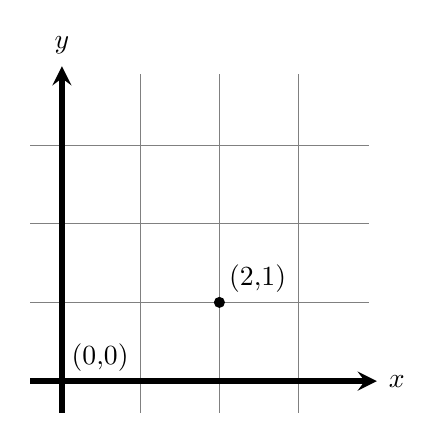
\begin{tikzpicture}
\draw[help lines,step=1cm,very thin](-0.4cm,-0.4cm)grid(3.9cm,3.9cm);
\draw[->,line width=0.7mm](-0.4cm,0)--(4cm,0)node[right]{$x$};
\draw[->,line width=0.7mm](0,-0.4cm)--(0,4cm)node[above]{$y$};
\draw (0,0)node[above right]{(0,0)};
\fill (2cm,1cm)node[above right]{(2,1)}circle(2pt);
\end{tikzpicture}}
\ffigbox{\caption{极坐标表示}\label{fig:jizuobiao1}}{
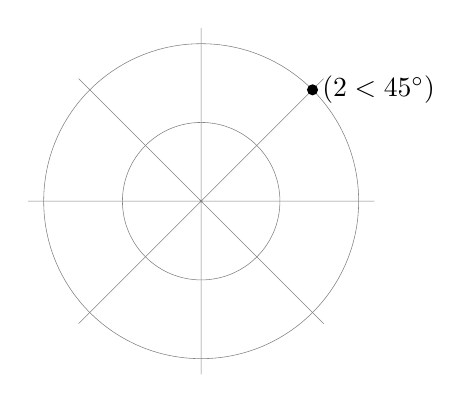
\begin{tikzpicture}
\draw[help lines,very thin](-2.2cm,0)--(2.2cm,0)(0,-2.2cm)--(0,2.2cm)(45:2.2cm)--(225:2.2cm)(135:2.2cm)--(-45:2.2cm);
\draw[help lines,very thin](0,0)circle(1cm)circle(2cm);
\fill (45:2cm)node[right]{$(2<45\degree)$}circle(2pt);
\end{tikzpicture}
}
\end{floatrow}
\end{figure}
\subsection{极坐标系}
极坐标系是一个二维坐标系统,它用一段相对于中心点的距离和一个夹角来表示坐标区域中的点,其坐形式为$(\rho,\theta)$,如图\ref{fig:jizuobiao1}所示。其中$\rho$表示距离,永远取正值,$\theta$表示角度,取值范围为$0-360\degree$。
\subsection{绝坐标和相对坐标}
绝对坐标是以当前坐标原点为基点进行参照所获得的坐标值。如$(3,5)$,$(4<45\degree)$。

相对坐标是以前面输入的坐标点为参照所获得的坐标值,表示方法是在坐标值前面加一个“@”符号。例如,相对直角坐标表示为$(@5,4)$,相对极坐标表示为$(@5<35)$。

例如,绘制一条两个端点分别为$(3,5)$和$(6,9)$的直线。调用line命令:

\noindent
命令: line 指定第一点: 3,5\\
指定下一点或 [放弃(U)]:\\
用绝对坐标方式输入,$(6,9)$就可以绘出直线。\\
用相对坐标方式输入,可知$(6,9)$相对于$(3,5)$的$X$轴增量为3,$Y$轴增量为4,故输入相对坐标$(@3,4)$也可以绘出直线。

\indent
但是,从AutoCAD的实际绘图过程来看,多种坐标输入方式配合使用会使整个绘图过程更加灵活和方便,再配合目标捕捉和夹点编辑等方式,则使绘图更精确、更快捷。
\zhishi{图纸幅面及格式}
\subsection{图纸幅面}
“图形界限”中我们所设置的297$\times $210的尺寸就是国家标准中的A4图纸幅面。国家标准《技术制图》中规定幅面的尺寸是为了方便绘制、使用和保管图样。因此,在绘制图样时,应优先采用表\ref{tab:tufubiao1}中规定的尺寸,必要时允许先用规定的加长幅面,加长幅面的尺寸由基本幅面短边的成整数倍增加后得出,如图\ref{fig:tufujiachang}所示。其中粗实细部分为基本幅面。加长后幅面记作:基本幅面代号$\times $倍数。如$A3\times 3$,表示按A3图幅短边加长为297mm的3倍,即加长后图纸尺寸为$420mm\times 891mm$。
%\suppressfloats[t]
\begin{table}[htbp]
\caption{图纸幅面及周边尺寸}\label{tab:tufubiao1}
\begin{tabular}{*{6}{c|}c}
\hline
\multicolumn{2}{c|}{幅面代号}&A0&A1&A2&A3&A4\\ \hline
\multicolumn{2}{c|}{尺寸 $B\times L$}&$841\times 1189$&$594\times 841$&$420\times 594$&$297\times 420$&$210\times 297$\\ \hline
\multirow{3}*{图框}&a&\multicolumn{5}{|c}{25}\\ \cline{2-7}
&c&\multicolumn{3}{|c}{10}&\multicolumn{2}{|c}{5}\\ \cline{2-7}
&e&\multicolumn{2}{|c}{20}&\multicolumn{3}{|c}{10}\\
\hline
\end{tabular}
\end{table}

\begin{figure}[htbp]
\centering
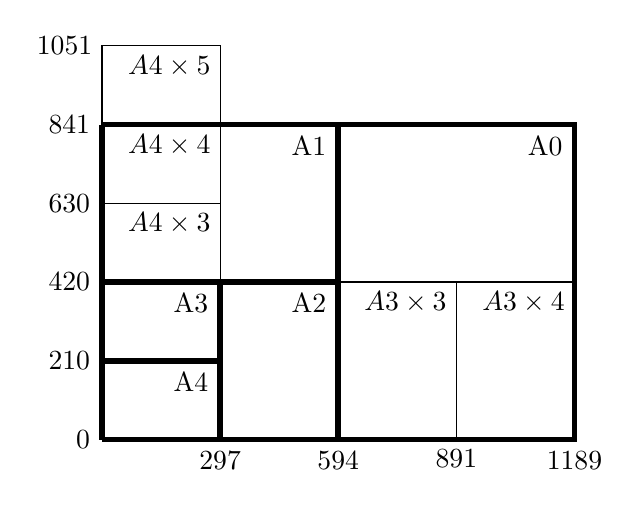
\begin{tikzpicture}
\draw[line width=0.7mm] (0,0)node[left]{0}--(0,1cm)node[left]{210}--(0,2cm)node[left]{420}--(0,3cm)node[left]{630}--(0,4cm)node[left]{841};
\draw(0,4cm)--(0,5cm)node[left]{1051}--(1.5cm,5cm)node[below left]{$A4\times 5$}--(1.5cm,2cm);
\draw[line width=0.7mm](0,1cm)--(1.5cm,1cm)node[below left]{A4}(0,2cm)--(1.5cm,2cm)node[below left]{A3}--(1.5cm,0)node[below]{297};
\draw(0,3cm)--(1.5cm,3cm)node[below left]{$A4\times 3$};
\draw[line width=0.7mm](0,4cm)--(3cm,4cm)node[below left]{A1}--(3cm,0)node[below]{594}(1.5cm,2cm)--(3cm,2cm)node[below left]{A2};
\draw[line width=0.7mm](3cm,4cm)--(6cm,4cm)node[below left]{A0}--(6cm,0)node[below]{1189}--(0,0);
\draw(3cm,2cm)--(4.5cm,2cm)node[below left]{$A3\times 3$}--(6cm,2cm)node[below left]{$A3\times 4$}(4.5cm,2cm)--(4.5cm,0)node[below]{891};
\draw(1.5cm,4cm)node[below left]{$A4\times 4$};
\end{tikzpicture}
\caption{图纸幅面及加长边} \label{fig:tufujiachang}
\end{figure}

从表\ref{tab:tufubiao1}中可以看出幅面之间的关系为:将A0图纸的长边对折后得到两张A1图纸,将A1图纸的长边对折后得到两纸A2图纸,以此类推。

\subsection{标题栏}
每张图样上必须画出标题栏,标题栏位于图样的右下角,与看图的方向一致。

标题栏分为更必区、签字区、名称及代号区和其他区,如图\ref{fig:biaotilan}所示。
\tikzset{
>=latex,
center lines/.style={dash pattern=on 20pt off 3pt on 2pt off 3pt},
importance lines/.style={line width=1pt}
}
\noindent
\begin{figure}[htbp]
\begin{tikzpicture}[scale=0.65]
\draw[line width=0.7mm](0,0)rectangle(180mm,56mm);
\draw(0,7mm)--(12mm,7mm)--(40mm,7mm)--++(40mm,0);
\draw(6mm,3.5mm)node{\tiny 工艺};
\draw(46mm,3.5mm)node{\tiny 批准};
\draw(0,14mm)--++(80mm,0);
\draw(6mm,10.5mm)node{\tiny 审核};
\draw(0,21mm)--++(12mm,0)--++(12mm,0)--++(16mm,0)--++(12mm,0)--++(12mm,0)--++(16mm,0);
\draw(6mm,24.5mm)node{\tiny设计};
\draw(18mm,24.5mm)node{\tiny(签名)};
\draw(32mm,24.5mm)node{\tiny(年月日)};
\draw(46mm,24.5mm)node{\tiny标准化};
\draw(58mm,24.5mm)node{\tiny签名};
\draw(72mm,24.5mm)node{\tiny(年月日)};
\draw(12mm,0)--++(0,28mm)(24mm,0)--++(0,28mm)(40mm,0)--++(0,28mm)(52mm,0)--++(0,28mm)(64mm,0)--++(0,28mm)(80mm,0)--++(0,28mm);
\draw(0,28mm)--++(10mm,0)--++(10mm,0)--++(16mm,0)--++(16mm,0)--++(12mm,0)--++(16mm,0);
\draw(5mm,31.5mm)node{\tiny 标记};
\draw(15mm,31.5mm)node{\tiny 处数};
\draw(28mm,31.5mm)node{\tiny 分区};
\draw(44mm,31.5mm)node{\tiny 更改文件号};
\draw(56mm,31.5mm)node{\tiny 签名};
\draw(72mm,31.5mm)node{\tiny 年月日};
\draw(0,35mm)--++(80mm,0)(0,42mm)--++(80mm,0)(0,49mm)--++(80mm,0);
\draw(10mm,28mm)--++(0,28mm)(20mm,28mm)--++(0,28mm)(36mm,28mm)--++(0,28mm)(52mm,28mm)--++(0,28mm)(64mm,28mm)--++(0,28mm)(80mm,28mm)--++(0,28mm);
\draw(80mm,9mm)--++(50mm,0);
\draw(105mm,4.5mm)node{\tiny 共\quad张\quad第\quad张};
\draw(80mm,18mm)--++(26mm,0)--++(12mm,0)--++(12mm,0);
\draw(93mm,23mm)node{\tiny 阶段标记};
\draw(112mm,23mm)node{\tiny 重量};
\draw(124mm,23mm)node{\tiny 比例};
\draw(86.5mm,9mm)--++(0,9mm)(93mm,9mm)--++(0,9mm)(99.5mm,9mm)--++(0,9mm)(106mm,9mm)--++(0,18mm)(118mm,9mm)--++(0,18mm);
\draw(80mm,28mm)--++(50mm,0);
\draw(130mm,0)--++(0,56mm);
\draw(130mm,18mm)--++(50mm,0)(130mm,38mm)--++(50mm,0);
\draw (155mm,9mm)node{\tiny(图样代号)};
\draw(155mm,28mm)node{\tiny(图样名称)};
\draw(155mm,48mm)node{\tiny(单位名称)};
\draw(105mm,48mm)node{\tiny(材料标记)};
\draw[<->](99.5mm,12mm)--(106mm,12mm)node[midway,above]{\tiny 6.5};
\draw(-14mm,0)--(0,0)(-7mm,7mm)--(0,7mm)(-14mm,56mm)--(0,56mm);
\draw[<->](-5mm,0)--(-5mm,7mm)node[midway,above,rotate=90]{\tiny 7};
\draw[<->](-13mm,0)--(-13mm,56mm)node[midway,above,rotate=90]{\tiny $8\times 7(56)$};
\draw(130mm,9mm)--++(9mm,0)(130mm,28mm)--++(9mm,0);
\draw[<->](137mm,0)--++(0,9mm)node[midway,above,rotate=90]{\tiny 9};
\draw[<->](137mm,9mm)--++(0,9mm)node[midway,above,rotate=90]{\tiny 9};
\draw[<->](137mm,18mm)--++(0,10mm)node[midway,above,rotate=90]{\tiny 10};
\draw(180mm,0)--++(9mm,0)(180mm,18mm)--++(9mm,0)(180mm,38mm)--++(9mm,0);
\draw[<->](187mm,0)--++(0,18mm)node[midway,above,rotate=90]{\tiny 18};
\draw[<->](187mm,18mm)--++(0,20mm)node[midway,above,rotate=90]{\tiny 20};
\draw(0,-9mm)--++(0,9mm)(12mm,-9mm)--++(0,9mm)(24mm,-9mm)--++(0,9mm)(40mm,-9mm)--++(0,9mm)(52mm,-9mm)--++(0,9mm)(64mm,-9mm)--++(0,9mm)(80mm,-9mm)--++(0,9mm)(130mm,-9mm)--++(0,9mm);
\draw[<->](0,-7mm)--++(12mm,0)node[midway,above]{\tiny 12};
\draw[<->](12mm,-7mm)--++(12mm,0)node[midway,above]{\tiny 12};
\draw[<->](24mm,-7mm)--++(16mm,0)node[midway,above]{\tiny 16};
\draw[<->](40mm,-7mm)--++(12mm,0)node[midway,above]{\tiny 12};
\draw[<->](52mm,-7mm)--++(12mm,0)node[midway,above]{\tiny 12};
\draw[<->](64mm,-7mm)--++(16mm,0)node[midway,above]{\tiny 16};
\draw[<->](80mm,-7mm)--++(50mm,0)node[midway,above]{\tiny 50};
\draw(0,-18mm)--(0,0)(180mm,-18mm)--(180mm,0);
\draw[<->](0,-16mm)--(180mm,-16mm)node[midway,above]{\tiny 180};
\draw(0,56mm)--++(0,7mm)(10mm,56mm)--++(0,7mm)(20mm,56mm)--++(0,7mm)(36mm,56mm)--++(0,7mm)(52mm,56mm)--++(0,7mm)(64mm,56mm)--++(0,7mm)(80mm,56mm)--++(0,7mm);
\draw[<->](0,61mm)--++(10mm,0)node[midway,above]{\tiny 10};
\draw[<->](10mm,61mm)--++(10mm,0)node[midway,above]{\tiny 10};
\draw[<->](20mm,61mm)--++(16mm,0)node[midway,above]{\tiny 16};
\draw[<->](36mm,61mm)--++(16mm,0)node[midway,above]{\tiny 16};
\draw[<->](52mm,61mm)--++(12mm,0)node[midway,above]{\tiny 12};
\draw[<->](64mm,61mm)--++(16mm,0)node[midway,above]{\tiny 16};
\draw(106mm,28mm)--++(0,7mm)(118mm,28mm)--++(0,7mm);
\draw[<->](80mm,33mm)--++(26mm,0)node[midway,above]{\tiny $4\times 6.5(26)$};
\draw[<->](106mm,33mm)--++(12mm,0)node[midway,above]{\tiny 12};
\draw[<->](118mm,33mm)--++(12mm,0)node[midway,above]{\tiny 12};
\end{tikzpicture}
\caption{标题栏格式及尺寸}\label{fig:biaotilan}
\end{figure}
\indent

\subsection{图框格式}
图框格式分为留装订边和不留装订边两种,其装订边尺寸如表\ref{tab:tufubiao1}所示。图\ref{fig:zhuangding}所示为采用A4幅面竖装和A3幅面横装时,留装订边和不留装订边的图框格式。
\noindent
\tikzset{
>=latex,
center lines/.style={dash pattern=on 20pt off 3pt on 2pt off 3pt},
importance lines/.style={line width=1pt}
}
\begin{figure}[htbp]
\centering
\subfloat[留装订边格式]{
\begin{tikzpicture}
\draw(0,0)rectangle(4cm,5cm);
\draw[line width=0.7mm](0.5cm,0.25cm)rectangle(3.75cm,4.75cm)(1.5cm,0.25cm)--(1.5cm,1cm)--(3.75cm,1cm)node[midway,below]{标题栏};
\draw(-0.7cm,0)--(0,0)(-0.7cm,5cm)--(0cm,5cm);
\draw[<->](-0.5cm,0)--(-0.5cm,5cm)node[midway,above,rotate=90]{$L$};
\draw(0,-0.7cm)--(0,0)(4cm,-0.7cm)--(4cm,0);
\draw[<->](0,-0.5cm)--(4cm,-0.5cm)node[midway,above]{$B$};
\draw[->](1cm,-0.45cm)--(1cm,0);
\draw[->](1cm,0.65cm)--(1cm,0.25cm)node[midway,above,rotate=90]{$c$};
\draw(1cm,0)--(1cm,0.25cm);
\draw[->](-0.4cm,2cm)--(0,2cm);
\draw[->](0.9cm,2cm)--(0.5cm,2cm);
\draw(0,2cm)--(0.5cm,2cm)node[midway,above]{$a$};
\draw[->](2cm,5cm)--(2cm,4.35cm)--(2cm,4.75cm);
\draw[->](2cm,5.45cm)--(2cm,5cm)node[midway,above,rotate=90]{$c$};
\draw[->](4cm,2.5cm)--(3.3cm,2.5cm)--(3.75cm,2.5cm);
\draw[->](4.45cm,2.5cm)--(4cm,2.5cm)node[midway,above]{$c$};

\begin{scope}[xshift=5.5cm]
\draw(0,0)rectangle(7cm,5cm);
\draw[line width=0.7mm](0.5cm,0.25cm)rectangle(6.75cm,4.75cm)(4.5cm,0.25cm)--(4.5cm,1cm)--(6.75cm,1cm)node[midway,below]{标题栏};
\draw(-0.7cm,0)--(0,0)(-0.7cm,5cm)--(0cm,5cm);
\draw[<->](-0.5cm,0)--(-0.5cm,5cm)node[midway,above,rotate=90]{$B$};
\draw(0,-0.7cm)--(0,0)(7cm,-0.7cm)--(7cm,0);
\draw[<->](0,-0.5cm)--(7cm,-0.5cm)node[midway,above]{$L$};
\draw[->](3cm,-0.45cm)--(3cm,0);
\draw[->](3cm,0.65cm)--(3cm,0.25cm)node[midway,above,rotate=90]{$c$};
\draw(3cm,0)--(3cm,0.25cm);
\draw[->](-0.4cm,2cm)--(0,2cm);
\draw[->](0.9cm,2cm)--(0.5cm,2cm);
\draw(0,2cm)--(0.5cm,2cm)node[midway,above]{$a$};
\draw[->](3.5cm,5cm)--(3.5cm,4.35cm)--(3.5cm,4.75cm);
\draw[->](3.5cm,5.45cm)--(3.5cm,5cm)node[midway,above,rotate=90]{$c$};
\draw[->](7cm,2.5cm)--(6.3cm,2.5cm)--(6.75cm,2.5cm);
\draw[->](7.45cm,2.5cm)--(7cm,2.5cm)node[midway,above]{$c$};
\end{scope}
\end{tikzpicture}}

\subfloat[不留装订边格式]{
\begin{tikzpicture}
\draw(0,0)rectangle(4cm,5cm);
\draw[line width=0.7mm](0.25cm,0.25cm)rectangle(3.75cm,4.75cm)(1.5cm,0.25cm)--(1.5cm,1cm)--(3.75cm,1cm)node[midway,below]{标题栏};
\draw(-0.7cm,0)--(0,0)(-0.7cm,5cm)--(0cm,5cm);
\draw[<->](-0.5cm,0)--(-0.5cm,5cm)node[midway,above,rotate=90]{$L$};
\draw(0,-0.7cm)--(0,0)(4cm,-0.7cm)--(4cm,0);
\draw[<->](0,-0.5cm)--(4cm,-0.5cm)node[midway,above]{$B$};
\draw[->](1cm,-0.45cm)--(1cm,0);
\draw[->](1cm,0.65cm)--(1cm,0.25cm)node[midway,above,rotate=90]{$c$};
\draw(1cm,0)--(1cm,0.25cm);
\draw[->](-0.4cm,2cm)--(0,2cm);
\draw[->](0.65cm,2cm)--(0.25cm,2cm)node[midway,above]{$c$};
\draw(0,2cm)--(0.25cm,2cm);
\draw[->](2cm,5cm)--(2cm,4.35cm)--(2cm,4.75cm);
\draw[->](2cm,5.45cm)--(2cm,5cm)node[midway,above,rotate=90]{$c$};
\draw[->](4cm,2.5cm)--(3.3cm,2.5cm)--(3.75cm,2.5cm);
\draw[->](4.45cm,2.5cm)--(4cm,2.5cm)node[midway,above]{$c$};

\begin{scope}[xshift=5.5cm]
\draw(0,0)rectangle(7cm,5cm);
\draw[line width=0.7mm](0.25cm,0.25cm)rectangle(6.75cm,4.75cm)(4.5cm,0.25cm)--(4.5cm,1cm)--(6.75cm,1cm)node[midway,below]{标题栏};
\draw(-0.7cm,0)--(0,0)(-0.7cm,5cm)--(0cm,5cm);
\draw[<->](-0.5cm,0)--(-0.5cm,5cm)node[midway,above,rotate=90]{$B$};
\draw(0,-0.7cm)--(0,0)(7cm,-0.7cm)--(7cm,0);
\draw[<->](0,-0.5cm)--(7cm,-0.5cm)node[midway,above]{$L$};
\draw[->](3cm,-0.45cm)--(3cm,0);
\draw[->](3cm,0.65cm)--(3cm,0.25cm)node[midway,above,rotate=90]{$c$};
\draw(3cm,0)--(3cm,0.25cm);
\draw[->](-0.4cm,2cm)--(0,2cm);
\draw[->](0.65cm,2cm)--(0.25cm,2cm)node[midway,above]{$c$};
\draw(0,2cm)--(0.25cm,2cm);
\draw[->](3.5cm,5cm)--(3.5cm,4.35cm)--(3.5cm,4.75cm);
\draw[->](3.5cm,5.45cm)--(3.5cm,5cm)node[midway,above,rotate=90]{$c$};
\draw[->](7cm,2.5cm)--(6.3cm,2.5cm)--(6.75cm,2.5cm);
\draw[->](7.45cm,2.5cm)--(7cm,2.5cm)node[midway,above]{$c$};
\end{scope}
\end{tikzpicture}}
\caption{图框格式}\label{fig:zhuangding}
\end{figure}
\indent
\clearpage
\section{平面几何作图(二)}

{\bfseries 知识目标}
\begin{itemize}
\item 掌握layger命令和图层定义和使用方法
\item 掌握xline命令的使用方法
\item 掌握circle命令的使用方法
\item 掌握多边形命令的使用方法
\item 掌握图形阵列命令的使用方法
\end{itemize}

{\bfseries 技能目标}
\begin{itemize}
\item 能够完成简单图样的绘制
\item 具备用AutoCAD图层管理图线的能力
\end{itemize}

\noindent
\begin{figure}[htbp]
\centering
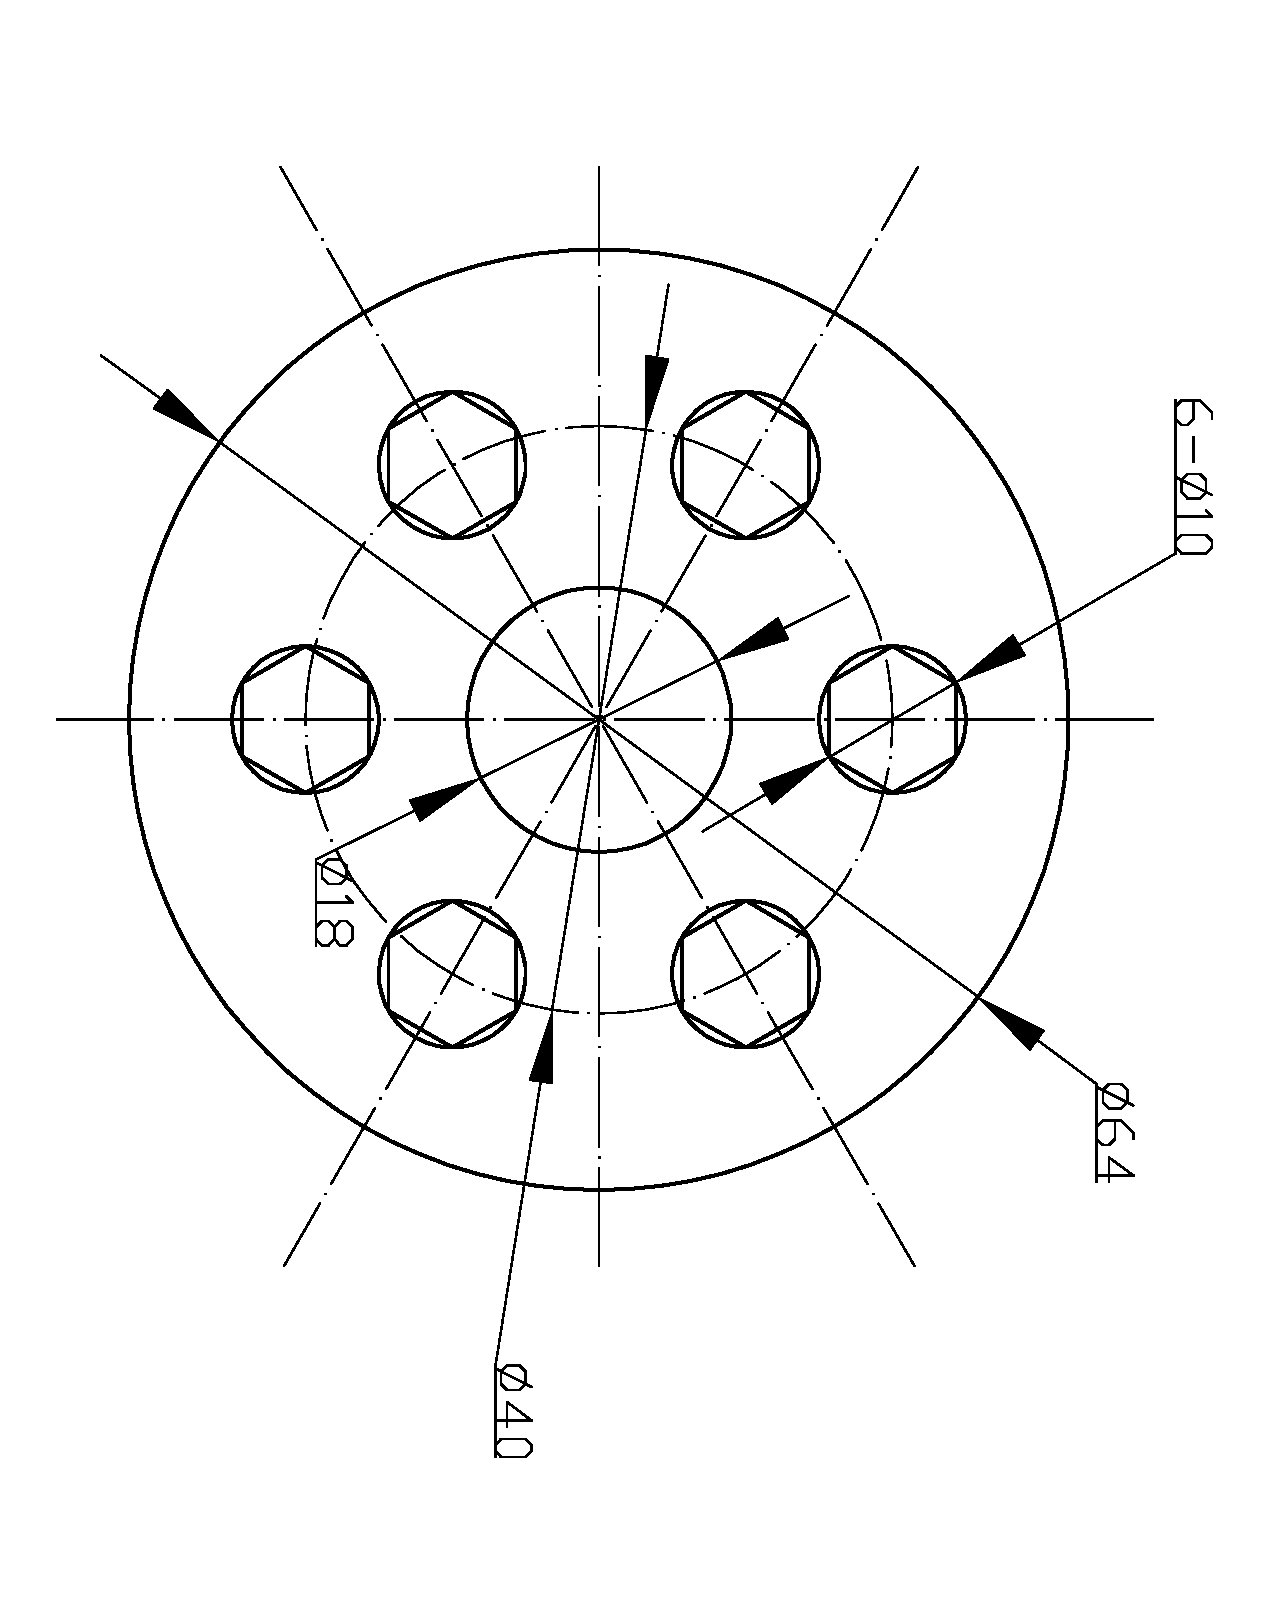
\includegraphics[scale=0.45,angle=90]{shu2.pdf}
\caption{任务二示例}\label{fig:renwu2}
\end{figure}

\indent
本任务以完成\ref{fig:renwu2}所示法兰盘图形为目标,旨在让读者掌握用AutoCAD的图层来管理各种图线,并学会构造线、圆、多边形和图形阵列编辑命令的使用技巧。并让读者认识和理解图样抄画的步骤和顺序,形成图样绘制的基本职业习惯。

\subsection{图层设置与管理}
\subsection{绘制图样}
\endinput

\section{电气元件}\label{sec:dianqiyuanjian}

{\bfseries 知识目标}
\begin{itemize}
\item 掌握图块的概念
\item 掌握图块的定义、插入、输出方法
\item 掌握图块属性定义与设置知识
\end{itemize}

{\bfseries 技能目标}
\begin{itemize}
\item 能够完成电子元件元件的定制
\end{itemize}

本任务以绘制\ref{fig:zhumodianlu}所示电路图中的电子元件为目标,主要是帮助读者掌握AutoCAD的图块的概念,以便于在绘图过程中将大量重复的图形定义为图块,以提高图形的绘制速度。

\subsection{电容元件}
首先,让我们来绘制图\ref{fig:zhumodianlu}所示电路图中的电容元件。

第一步,先绘制电容元件的对称中心线。

\noindent
\begin{figure}[htbp]
\centering
\subfloat[]{\label{fig:dianrong1}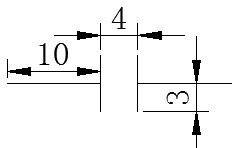
\includegraphics[scale=0.3]{dianrong1.png}}\hspace{20pt}
\subfloat[]{\label{fig:dianrong2}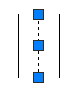
\includegraphics[scale=0.5]{dianrong2.png}}\hspace{20pt}
\subfloat[]{\label{fig:dianrong3}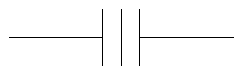
\includegraphics[scale=0.5]{dianrong3.png}}
\subfloat[]{\label{fig:dianrong4}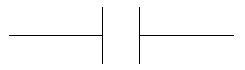
\includegraphics[scale=0.5]{dianrong4.png}}
\caption{电容元件绘制}
\end{figure}

\noindent
命令:line\\
指定第一点:\\
指定下一点或 [放弃(U)]: @6$<90$\\
指定下一点或 [放弃(U)]:\\
\indent

第二步,以对称中心做为偏移对象,向左右各偏移2mm,如图\ref{fig:dianrong2} 所示。

\noindent
命令: offset
当前设置: 删除源=否  图层=源  OFFSETGAPTYPE=0\\
指定偏移距离或 [通过(T)/删除(E)/图层(L)] $<$通过$>$:  2\\
选择要偏移的对象,或 [退出(E)/放弃(U)] $<$退出$>$:\\
指定要偏移的那一侧上的点,或 [退出(E)/多个(M)/放弃(U)] $<$退出$>$:\\
选择要偏移的对象,或 [退出(E)/放弃(U)] $<$退出$>$:\\
指定要偏移的那一侧上的点,或 [退出(E)/多个(M)/放弃(U)] $<$退出$>$:\\
选择要偏移的对象,或 [退出(E)/放弃(U)] $<$退出$>$:\\
\indent

第三步,绘电容接线时,以其最左侧竖线的中心点为起点向左绘制10mm的线条,然后以中心线做另一电容接线,最终结果如图\ref{fig:dianrong3}所示。

\noindent
命令: line\\
指定第一点: mid\\
于\\
指定下一点或 [放弃(U)]: @10$<$-180\\
指定下一点或 [放弃(U)]:\\
命令: mirror\\
选择对象: 找到 1 个\\
选择对象:  指定镜像线的第一点: 指定镜像线的第二点:\\
要删除源对象吗?[是(Y)/否(N)] $<N>:$

\indent
最后,删除中心线,完成电容元件的绘制,其结果如图\ref{fig:dianrong4}所示。

由于电器元件通常都需要重复使用,为了提高我们的绘图速度,需要将绘制的电气元件定义为块并写入文件中,才能够实现其重复利用的目的。下面我们将通过电容块的定义来说明块的定义过程。当我们输入block命令后,会出现图所示的块定义窗体。我们在窗体中命名块的名称为电容,点击拾取点并选择电容元件的最左点来完成基点的定义,点击选择对象并选整个电容图形来完成对象的定义,最后点击确定。

\noindent
命令: block 指定插入基点:\\
选择对象: 指定对角点: 找到 4 个\\
选择对象:\\

\indent
完成块定义后,还需要通过块写命令wblock将定义的块写入dwg文件中才能够实现随时调用和重复利用。
\subsection{接地元件}

\subsection{电阻元件}

\subsection{电灯元件}

\subsection{二极管元件}

\subsection{三极管元件}

\section{触摸延时开关电路图}

\endinput
\section{旋转建模法}
\subsection{绘制左视图}
\begin{procedure}
\item 设置图层,新建“中心线”和“实线”两个图层,具体设计请参看\ref{sec:dianpian}节的图层设置相关内容。
\item  切换视图为主视图。【视图】菜单中【三维视图】子菜单中的【左视图】。
\item 绘制中心线,其结果如图\ref{fig:dianpiancenterline1}所示。
\begin{lstlisting}
|命令: xline|
|指定点或 [水平(H)/垂直(V)/角度(A)/二等分(B)/偏移(O)]:|
|指定通过点:$@1<0$|
|指定通过点:$@1<90$|
|指定通过:|
|命令:OFFSET|
|当前设置: 删除源=否  图层=源  OFFSETGAPTYPE=0|
|指定偏移距离或 [通过(T)/删除(E)/图层(L)] $<$通过$>$:  42|
|选择要偏移的对象,或 [退出(E)/放弃(U)] $<$退出$>$:|
|指定要偏移的那一侧上的点,或 [退出(E)/多个(M)/放弃(U)] $<$退出$>$:|
|选择要偏移的对象,或 [退出(E)/放弃(U)] $<$退出$>$:
\end{lstlisting}
\item 将图层切换为实线层
\begin{figure}[htbp]
\centering
\subfloat[]{\label{fig:dianpiancenterline1}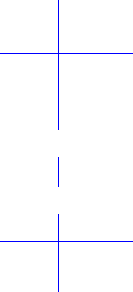
\includegraphics[scale=0.6]{dianpiancenterline1.png}}\hspace{40pt}
\subfloat[]{\label{fig:dianpianleft1}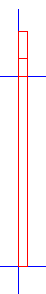
\includegraphics[scale=0.6]{dianpianleft1.png}}
\caption{垫片左视图绘制}
\end{figure}
\item 使用【矩形】命令绘制左视图中的关键特征,其结果如图\ref{fig:dianpianleft1}所示。【矩形】命令的启动方法有:
\begin{itemize}
\item 键盘输入RECTANGLE或REC
\item 点击【绘图】菜单中的【矩形】项。
\item 点击【绘图】工具栏中的【矩形】图标
\includegraphics[scale=0.6]{rectangletool.png}
\end{itemize}
\begin{lstlisting}
|命令: rectang|
|指定第一个角点或 [倒角(C)/标高(E)/圆角(F)/厚度(T)/宽度(W)]:|
|指定另一个角点或 [面积(A)/尺寸(D)/旋转(R)]: @2,52|
|命令: rectang|
|指定第一个角点或 [倒角(C)/标高(E)/圆角(F)/厚度(T)/宽度(W)]:|
|指定另一个角点或 [面积(A)/尺寸(D)/旋转(R)]: @2,4|
|命令: rectang|
|指定第一个角点或 [倒角(C)/标高(E)/圆角(F)/厚度(T)/宽度(W)]:|
|指定另一个角点或 [面积(A)/尺寸(D)/旋转(R)]: @2,26.5|
\end{lstlisting}
\end{procedure}

\subsection{旋转构建垫片的三维模型}
\begin{procedure}
\item 通过建模中的【旋转】操作产生两个圆柱。
\begin{lstlisting}
|命令: REVOLVE|
|当前线框密度:  ISOLINES=4,闭合轮廓创建模式 = 实体|
|选择要旋转的对象或 [模式(MO)]: 找到 1 个|
|选择要旋转的对象或 [模式(MO)]:|
|指定轴起点或根据以下选项之一定义轴 [对象(O)/X/Y/Z] $<$对象$>$:|
|指定轴端点:|
|指定旋转角度或 [起点角度(ST)/反转(R)/表达式(EX)] $<360>$:|
|命令:  REVOLVE|
|当前线框密度:  ISOLINES=4,闭合轮廓创建模式 = 实体|
|选择要旋转的对象或 [模式(MO)]: 找到 1 个|
|选择要旋转的对象或 [模式(MO)]:|
|指定轴起点或根据以下选项之一定义轴 [对象(O)/X/Y/Z] $<$对象$>$:|
|指定轴端点:|
|指定旋转角度或 [起点角度(ST)/反转(R)/表达式(EX)]$ <360>$:|
\end{lstlisting}
\item 关闭“中心线”图层。
\item 切换视图为西南等轴测图。点击【视图】菜单中【三维视图】子菜单中的【西南等轴测】。切换后的结果如图\ref{fig:3darray}所示。
\begin{figure}[htbp]
\centering
\subfloat[]{\label{fig:3darray}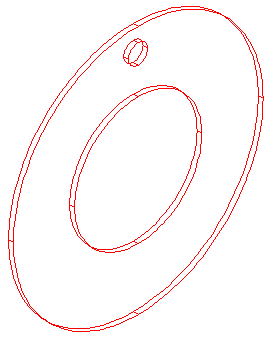
\includegraphics[scale=0.5]{3darray.png}}\hspace{30pt}
\subfloat[]{\label{fig:3darrayselect}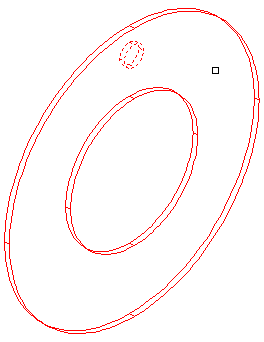
\includegraphics[scale=0.5]{3darrayselect.png}}\hspace{30pt}
\subfloat[]{\label{fig:3darrayresult}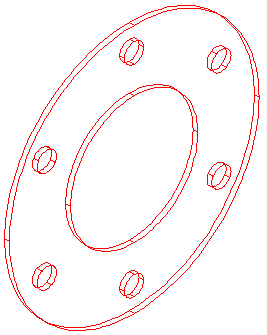
\includegraphics[scale=0.5]{3darrayresult.png}}
\caption{三维阵列过程}
\end{figure}
\item 用【三维阵列】命令阵列$\diameter 8$的圆柱,其结果如图\ref{fig:3darrayresult}所示。启动【三维阵列】命令的方法有:
\begin{itemize}
\item 键盘输入3DARRAY
\item 点击【修改】菜单【三维操作】子菜单中的【三维阵列】项。
\item 点击【建模】工具栏中的【三维阵列】图标
\includegraphics[scale=0.6]{3darraytool.png}
\end{itemize}
\begin{lstlisting}
|命令: 3darray|
|选择对象: 找到 1 个\longremark{选择$\diameter 8$圆柱,如图\ref{fig:3darrayselect}所示。}|
|选择对象:|
|输入阵列类型 [矩形(R)/环形(P)]$<$矩形$>$:p|
|输入阵列中的项目数目: 6|
|指定要填充的角度 (+=逆时针, -=顺时针)$ <360>$:|
|旋转阵列对象? [是(Y)/否(N)] $<Y>$:|
|指定阵列的中心点:\longremark{选择$\diameter 104$圆柱的后底圆圆心。}|
|指定旋转轴上的第二点:\longremark{选择$\diameter 104$圆柱的后底圆圆心。}|
\end{lstlisting}
\showremarks
\item 用差集操作完成垫片的三维建模操作。
\begin{lstlisting}
|命令: subtract |
|选择要从中减去的实体、曲面和面域...|
|选择对象: 找到 1 个|
|选择对象:  选择要减去的实体、曲面和面域...|
|选择对象: 找到 1 个|
|选择对象: 找到 1 个,总计 2 个|
|选择对象: 找到 1 个,总计 3 个|
|选择对象: 找到 1 个,总计 4 个|
|选择对象: 找到 1 个,总计 5 个|
|选择对象: 找到 1 个,总计 6 个|
|选择对象: 找到 1 个,总计 7 个|
|选择对象:|
\end{lstlisting}
\item 设置视觉样式为真实,其结果如图\ref{fig:dianpiansolid}所示。设置方法为:点击【视图】菜单中【视觉样式】子菜单中的【真实】项。
\item 将垫片模型保存为“调压阀垫片立体图.dwg”。
\end{procedure}

\endinput
%%%%%%%%%%%%%%%教案头%%%%%%%%%%%%%%%%%%%%%%%%%%%%%%%
\mode<article>{

\begin{longtable}{|m{20mm}|m{20mm}|m{20mm}|m{20mm}|m{20mm}|m{28mm}|}
\caption*{\huge 教案头}\\
\hline
\endfirsthead
\multicolumn{6}{l}{(续表)}\\
\hline
\endhead
\hline
\multicolumn{6}{l}{\itshape 接下一页表格.......}\\ [2ex]
\endfoot
\hline
\endlastfoot
\centering{授课单元}&\multicolumn{3}{m{60mm}|}{\centering 2.4.4方框图简化}&\centering{授课日期}&2014年03月13日 \\
\hline
\centering 授课地点 & \multicolumn{3}{m{60mm}|}{B6-204}&\centering 授课学时 & 2 \\
\hline
& \multicolumn{2}{m{40mm}|}{能力目标} & \multicolumn{2}{m{40mm}|}{知识目标}&素质目标 \\
\cline{2-6}
\centering 教学目标&\multicolumn{2}{m{40mm}|}{\begin{enumerate}
\item 能够进行方框图的简化
\end{enumerate} }&\multicolumn{2}{m{40mm}|}{\begin{enumerate}
\item 掌握方框图简化的方法
\end{enumerate}} & {\qquad}\\
\hline
\centering 能力训练任务或案例 &\multicolumn{5}{m{108mm}|}{\begin{enumerate}
\item RC网络电路图
\item RLC网络电路图
\end{enumerate}}\\
\hline
\centering 教学重点 & \multicolumn{5}{m{108mm}|}{\begin{enumerate}
\item 方框图的传递函数
\item 方框图的绘制
\end{enumerate}}\\
\hline
\centering 教学难点与解决办法 &\multicolumn{5}{m{108mm}|}{\begin{enumerate}
\item 难点:方框图的绘制
\item 解决方法:用实例进行分析讲解
\end{enumerate}}\\
\hline
\centering 德育内容 &\multicolumn{5}{m{108mm}|}{无}\\
\hline
 &教材 & \multicolumn{4}{m{88mm}|}{计算机控制原理与应用}\\
\cline{2-6}& 教学资源 &\multicolumn{4}{m{88mm}|}{PPT}\\
\cline{2-6}\centering 使用的教学材料& 主要教学仪器设备和工具等 &\multicolumn{4}{m{88mm}|}{投影机、MATLAB}\\
\cline{2-6}& 主要耗材 &\multicolumn{4}{m{88mm}|}{无}\\
\hline
\centering 教学模式 &\multicolumn{2}{m{40mm}|}{知识讲授}&\centering 教学手段 &\multicolumn{2}{m{48mm}|}{多媒体教学}\\
\hline
\centering 学生成果与过程考核方式 &\multicolumn{5}{m{108mm}|}{无}
\end{longtable}
\clearpage

%%%%%%%%%%%%%%%教学实施过程%%%%%%%%%%%%%%%%%%%%%%%%%%%%
\begin{landscape}

\begin{longtable}{|m{10mm}|m{50mm}|m{50mm}|m{50mm}|m{15mm}|}
\caption*{\huge 教学组织与实施}\\
\hline
\endfirsthead
\multicolumn{5}{l}{\small 接上页}\\
\hline
\multicolumn{1}{|c|}{步骤}&\multicolumn{1}{c|}{教学内容}&\multicolumn{1}{c|}{教师活动}&\multicolumn{1}{c|}{学生活动}&\multicolumn{1}{c|}{时间}\\
\hline
\endhead

\multicolumn{5}{r}{\small 接下页}\\
\endfoot
\hline
\endlastfoot
\multicolumn{1}{|c|}{步骤}&\multicolumn{1}{c|}{教学内容}&\multicolumn{1}{c|}{教师活动}&\multicolumn{1}{c|}{学生活动}&\multicolumn{1}{c|}{时间}\\\hline
引入&\begin{enumerate}
\item 分析系统微分方程存在的不足
\end{enumerate} &\begin{enumerate}
\item 系统微分方程不便于表示复杂的系统
\item 建立比较复杂
\item 不便于进行系统特性分析
\end{enumerate} &\begin{enumerate}
\item 学生记录
\end{enumerate} &10 \\\hline
讲解&\begin{enumerate}
\item 传递函数和微分方程
\end{enumerate}
 &\begin{enumerate}
\item 通过数学推导讲明传递函数与微分方程之间的关系
\end{enumerate} &\begin{enumerate}
\item 学生倾听并记录
\end{enumerate} &15 \\\hline
讲解&\begin{enumerate}
\item 电子网络的传递函数
\end{enumerate}
&\begin{enumerate}
\item 展示RC和RCL电子网络电路图
\item 指导学生求取传递函数
\item 讲解求取要点
\end{enumerate} &\begin{enumerate}
\item 学生尝试求取传递函数
\item 学生展示传递函数的结果
\item 学生进行记录
\end{enumerate} &20 \\\hline
讲解&\begin{enumerate}
\item 简单方框图的传递函数
\end{enumerate}
 &\begin{enumerate}
\item 讲解方框图的概念
\item 讲解方框图传递函数的求取方法
\end{enumerate} &\begin{enumerate}
\item 学生记录笔记
\end{enumerate} &20 \\\hline
讲解&
\begin{enumerate}
\item 方框图的绘制
\end{enumerate}
 &\begin{enumerate}
\item 以RC电路为例讲解方框图的绘方法
\item 指导学生绘制RLC电路的方框图
\item 讲解要点
\end{enumerate} &\begin{enumerate}
\item 学生倾听并记录
\item 学生尝试绘制RLC电路的方框图
\item 学生记录笔记
\end{enumerate} &20 \\\hline
\centering 本次课总结(评价)&总结本课程内容 &进行知识总结 &学生倾听 &5 \\\hline
\centering 学生学习笔记或工单等检查情况&\multicolumn{4}{m{165mm}|}{\quad}\\\hline
\centering 课后作业&\multicolumn{4}{m{165mm}|}{2-19,2-20,2-21}\\\hline
\centering 教学体会&\multicolumn{4}{m{165mm}|}{\quad}\\
\end{longtable}

\end{landscape}
\clearpage
%%%%%%%%%%%%%%%%%%%%板书设计%%%%%%%%%%%%%%%%%%%%%%%%%%
\lecture{传递函数与方框图}{chuandihanshu}
\begin{center}
{\huge 板书设计}
\end{center}
}
\mode<presentation>{ \section{传递函数与微分方程}
 \subsection{传递函数和微分方程}}
 \begin{frame}[containsverbatim]{传递函数和微分方程}
\begin{eqnarray*}
 \frac{d^n y(t)}{dt^n}+a_1\frac{d^{n-1}y(t)}{dt^{n-1}}+\cdots \\ 
 +a_{n-1}\frac{dy(t)}{dt}+a_ny(t)=
 \\  b_0\frac{d^mx(t)}{dt^m}+b_1\frac{d^{m-1}x(t)}{dt^{m-1}}+\cdots \\
 +b_{m-1}\frac{dx(t)}{dt}+b_mx(t)
 \end{eqnarray*}
 \end{frame}
 \begin{frame}
 \begin{eqnarray*}
 G(s)=\frac{Y(s)}{X(s)}\\ 
 =\frac{b_0s^m+b_1s^{m-1}+\cdots +b_{m-1}s+b_m}{s^n+a_1s^{n-1}+\cdots +a_{n-1}s+a_n}
 \end{eqnarray*}
 \end{frame}
 \begin{frame}{电子网络的传递函数}
 \begin{block}{RC无源网络}
 \[\frac{dV_2(t)}{dt}+\frac{1}{RC}V_2(t)=\frac{1}{RC}v_1(t)\]
 \[sV_2(s)+\frac{1}{RC}V_2(s)=\frac{1}{RC}V_1(s)\]
 \[\frac{V_2(s)}{V_1(s)}=\frac{1}{RCs+1}\]
 \end{block}
 \end{frame}
 \begin{frame}
 \begin{block}{RLC无源网络}
 \[\frac{d^2V_2(t)}{dt^2}+\frac{RdV_2(t)}{Ldt}+\frac{V_2(t)}{LC}=\frac{V_1(t)}{LC}
 \]
 \[\frac{V_2(s)}{V_1(s)}=\frac{1}{LCs^2+RCs+1}
 \]
 \end{block}
 \end{frame}
 \begin{frame}{简单方框图的传递函数}
 \begin{definition}
 \begin{itemize}
 \item 是一种图形
 \item 表示元件或子系统的功能
 \item 表示信号流向
 \end{itemize} 
 \end{definition}
 \begin{block}{方框图的特点}
 \begin{itemize}
 \item 保持系统的数学描述
 \item 信号流向用箭头表示
 \item 包含系统动态特性信息,不含物理结构
 \end{itemize} 
 \end{block}
 \end{frame}
 \begin{frame}{方框图的传递函数}
 \begin{block}{开环系统}
 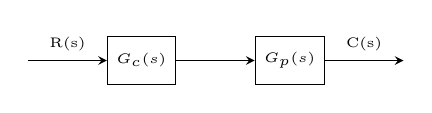
\begin{tikzpicture}
 [node distance=10mm,>=stealth]
 \node(GS1)[nonterminal]{\tiny $G_c(s)$};
 \draw[<-](GS1.west)--++(-10mm,0)node[midway,above]{\tiny R(s)};
 \node(GS2)[nonterminal,right=of GS1]{\tiny $G_p(s)$};
 \draw[->](GS1.east)--(GS2.west);node[midway,above]{\tiny M(s)};
 \draw[->](GS2.east)--++(10mm,0)node[midway,above]{\tiny C(s)};
 \end{tikzpicture}
 \end{block}
 \begin{block}{传递函数}
 \[G(s)=G_c(s)G_p(s)\]
 \end{block}
 \end{frame}
 \begin{frame}[allowframebreaks]
 \begin{block}{闭环系统}
 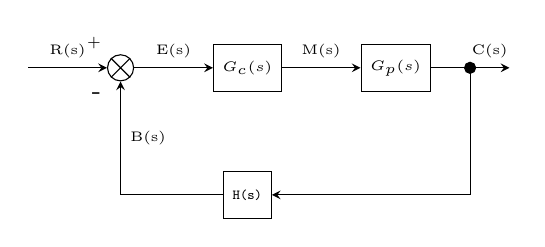
\begin{tikzpicture}
 [node distance=10mm,>=stealth]
 \node(star)[circleterminal,label=above left:\tiny +,label=below left:-]{};
 \draw(star.north east)--(star.south west)(star.south east)--(star.north west);
 \draw[<-](star.west)--++(-10mm,0)node[above,midway]{\tiny R(s)};
 \node(GS1)[nonterminal,right=of star]{\tiny $G_c(s)$};
 \draw[->](star.east)--(GS1.west)node[midway,above]{\tiny E(s)};
 \node(GS2)[nonterminal,right=of GS1]{\tiny $G_p(s)$};
 \draw[->](GS1.east)--(GS2.west)node[midway,above]{\tiny M(s)};
 \draw[->](GS2.east)--++(10mm,0)node[near end,above]{\tiny C(s)};
 \node(feadback)[nonterminal,below=of GS1]{\tiny H(s)};
 \draw[->]($(GS2.east)+(5mm,0)$)coordinate(a)|-(feadback.east);
 \filldraw(a)circle(2pt);
 \draw[->](feadback.west)-|(star.south)node[near end,right]{\tiny B(s)};
 \end{tikzpicture}
 \end{block}
 \begin{block}{传递函数}
 \[C(s)=E(s)G_c(s)G_p(s)\]
 \[B(s)=C(s)H(s)\]
 \[E(s)=R(s)-B(s)\]
 \[G(s)=\frac{G_c(s)G_p(s)}{1+G_c(s)G_p(s)H(s)}\]
 \end{block}
 \end{frame}
 \begin{frame}
 \begin{block}{方框图的画法}
 \begin{itemize}
 \item 找出被控对象
 \item 明确输入输出关系
 \item 找出控制环节
 \item 根据信号流连接各个环节
 \end{itemize}
 \end{block}
 \end{frame}
 \begin{frame}
 \begin{example}
 \begin{circuitikz}[american]
\draw(0,0)to[generic,l^=$R$,o-*](3,0)to[C,l=$C$](3,-2)to[short,*-o](0,-2)to[open,o-,l=$v_{1}(t)$](0,0)(3,0)to[short,-o](5,0)to[open,-o,l=$v_{o}(t)$](5,-2)to[short](3,-2);
\end{circuitikz}
\end{example}
 \end{frame}
\begin{frame}
\begin{block}{绘制电阻R控制图}
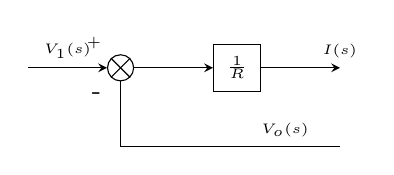
\begin{tikzpicture}
[node distance=10mm,>=stealth]
\node(start)[circleterminal,label=above left:\tiny +,label=below left:-]{};
\draw(start.north west)--(start.south east);
\draw(start.north east)--(start.south west);
\draw[<-](start.west)--++(-10mm,0)node[midway,above]{\tiny $V_1(s)$};
\node(R)[nonterminal,right=of start]{\tiny $\frac{1}{R}$};
\draw[->](start.east)--(R.west);
\draw[->](R.east)--++(10mm,0)coordinate(a)node[above]{\tiny $I(s)$};
\draw($(a)+(0,-10mm)$)-|(start.south)node[very near start,above]{\tiny $V_o(s)$}; 
\end{tikzpicture}
\end{block}
\begin{block}{加入电容C的控制图}
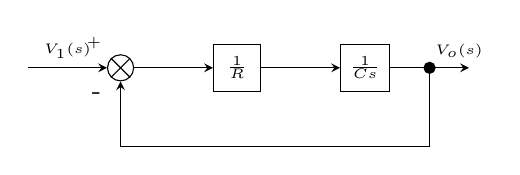
\begin{tikzpicture}
[node distance=10mm,>=stealth]
\node(start)[circleterminal,label=above left:\tiny +,label=below left:-]{};
\draw(start.north west)--(start.south east);
\draw(start.north east)--(start.south west);
\draw[<-](start.west)--++(-10mm,0)node[midway,above]{\tiny $V_1(s)$};
\node(R)[nonterminal,right=of start]{\tiny $\frac{1}{R}$};
\draw[->](start.east)--(R.west);
\node(C)[nonterminal,right=of R]{\tiny $\frac{1}{Cs}$};
\draw[->](R.east)--(C.west);
\draw[->](C.east)--++(10mm,0)coordinate(a)node[very near end,above]{\tiny $V_o(s)$};
\draw[->]($(C.east)!.5!(a)$)coordinate(b)--++(0,-10mm)-|(start.south);
\filldraw(b)circle(2pt);
\end{tikzpicture}
\end{block}
\end{frame}
\begin{frame}
\begin{example}
\begin{circuitikz}[american]
 \draw(0,0)to[generic,l^=$R$,o-](2,0)to[L,l^=$L$](4,0)to[C,l=$C$,*-*](4,-2)to[short,-o](0,-2)to[open,l=$v_{1}(t)$](0,0)(4,0)to[short,-o](6,0)to[open,l=$v_{o}(t)$,-o](6,-2)to[short](4,-2);
 \end{circuitikz}
\end{example}
\end{frame}
\begin{frame}
\begin{block}{绘制电阻R控制图}
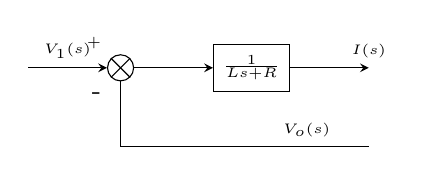
\begin{tikzpicture}
[node distance=10mm,>=stealth]
\node(start)[circleterminal,label=above left:\tiny +,label=below left:-]{};
\draw(start.north west)--(start.south east);
\draw(start.north east)--(start.south west);
\draw[<-](start.west)--++(-10mm,0)node[midway,above]{\tiny $V_1(s)$};
\node(R)[nonterminal,right=of start]{\tiny $\frac{1}{Ls+R}$};
\draw[->](start.east)--(R.west);
\draw[->](R.east)--++(10mm,0)coordinate(a)node[above]{\tiny $I(s)$};
\draw($(a)+(0,-10mm)$)-|(start.south)node[very near start,above]{\tiny $V_o(s)$}; 
\end{tikzpicture}
\end{block}
\begin{block}{加入电容C的控制图}
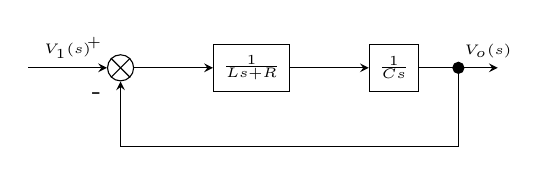
\begin{tikzpicture}
[node distance=10mm,>=stealth]
\node(start)[circleterminal,label=above left:\tiny +,label=below left:-]{};
\draw(start.north west)--(start.south east);
\draw(start.north east)--(start.south west);
\draw[<-](start.west)--++(-10mm,0)node[midway,above]{\tiny $V_1(s)$};
\node(R)[nonterminal,right=of start]{\tiny $\frac{1}{Ls+R}$};
\draw[->](start.east)--(R.west);
\node(C)[nonterminal,right=of R]{\tiny $\frac{1}{Cs}$};
\draw[->](R.east)--(C.west);
\draw[->](C.east)--++(10mm,0)coordinate(a)node[very near end,above]{\tiny $V_o(s)$};
\draw[->]($(C.east)!.5!(a)$)coordinate(b)--++(0,-10mm)-|(start.south);
\filldraw(b)circle(2pt);
\end{tikzpicture}
\end{block}
\end{frame}
\begin{frame}
\begin{block}{最终结果}
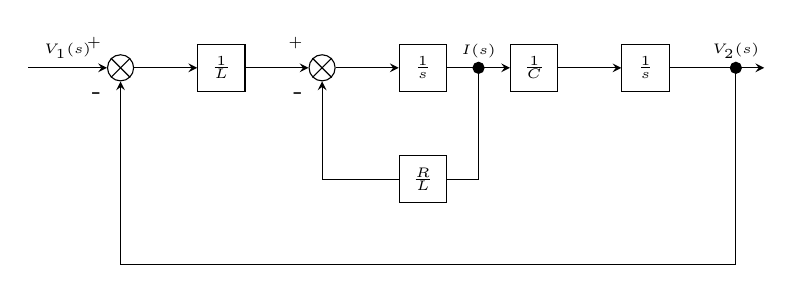
\begin{tikzpicture}
[node distance=8mm,>=stealth]
\node(start1)[circleterminal,label=above left:\tiny +,label=below left:-]{};
\draw(start1.north west)--(start1.south east);
\draw(start1.north east)--(start1.south west);
\draw[<-](start1.west)--++(-10mm,0)node[midway,above]{\tiny $V_1(s)$};
\node(L)[nonterminal,right=of start1]{\tiny $\frac{1}{L}$};
\draw[->](start1.east)--(L.west);
\node(start2)[circleterminal,label=above left:\tiny +,label=below left:-,right=of L]{};
\draw(start2.north west)--(start2.south east);
\draw(start2.north east)--(start2.south west);
\draw[->](L.east)--(start2.west);
\node(S)[nonterminal,right=of start2]{\tiny $\frac{1}{s}$};
\draw[->](start2.east)--(S.west);
\node(C)[nonterminal,right=of S]{\tiny $\frac{1}{C}$};
\draw[->](S.east)--(C.west);
\node(fback)[nonterminal,below=of S]{\tiny $\frac{R}{L}$};
\draw($(S.east)!.5!(C.west)$)coordinate(a)node[above]{\tiny $I(s)$}|-(fback.east);
\draw[->](fback.west)-|(start2.south);
\filldraw(a)circle(2pt);
\node(S1)[nonterminal,right=of C]{\tiny $\frac{1}{s}$};
\draw[->](C.east)--(S1.west);
\draw[->](S1.east)--++(12mm,0)coordinate(b);
\draw[->]($(S1.east)!.7!(b)$)coordinate(c)node[above]{\tiny $V_2(s)$}--++(0,-25mm)-|(start1.south);
\filldraw(c)circle(2pt);
\end{tikzpicture}
\end{block}
\end{frame}
%%%%%%%%%%%%%%教案头%%%%%%%%%%%%%%%%%%%%%%%%%%%%%%%
\mode<article>{

\begin{longtable}{|m{20mm}|m{20mm}|m{20mm}|m{20mm}|m{20mm}|m{28mm}|}
\caption*{\huge 教案头}\\
\hline
\endfirsthead
\multicolumn{6}{l}{(续表)}\\
\hline
\endhead
\hline
\multicolumn{6}{l}{\itshape 接下一页表格.......}\\ [2ex]
\endfoot
\hline
\endlastfoot
\centering{授课单元}&\multicolumn{3}{m{60mm}|}{\centering 2.5传递函数和信号流图}&\centering{授课日期}&2014年03月13日 \\
\hline
\centering 授课地点 & \multicolumn{3}{m{60mm}|}{B6-204}&\centering 授课学时 & 2 \\
\hline
& \multicolumn{2}{m{40mm}|}{能力目标} & \multicolumn{2}{m{40mm}|}{知识目标}&素质目标 \\
\cline{2-6}
\centering 教学目标&\multicolumn{2}{m{40mm}|}{\begin{enumerate}
\item 能够将方框图转化为信号流图
\item 能够应用梅逊增益公式求解系统的传递函数
\end{enumerate} }&\multicolumn{2}{m{40mm}|}{\begin{enumerate}
\item 掌握信号流图的画法
\item 掌握梅逊增益公式
\end{enumerate}} & {\qquad}\\
\hline
\centering 能力训练任务或案例 &\multicolumn{5}{m{108mm}|}{ }\\
\hline
\centering 教学重点 & \multicolumn{5}{m{108mm}|}{\begin{enumerate}
\item 梅逊增益公式
\end{enumerate}}\\
\hline
\centering 教学难点与解决办法 &\multicolumn{5}{m{108mm}|}{\begin{enumerate}
\item 难点:梅逊增益公式
\item 解决方法:用实例进行分析讲解
\end{enumerate}}\\
\hline
\centering 德育内容 &\multicolumn{5}{m{108mm}|}{无}\\
\hline
 &教材 & \multicolumn{4}{m{88mm}|}{计算机控制原理与应用}\\
\cline{2-6}& 教学资源 &\multicolumn{4}{m{88mm}|}{PPT}\\
\cline{2-6}\centering 使用的教学材料& 主要教学仪器设备和工具等 &\multicolumn{4}{m{88mm}|}{投影机、MATLAB}\\
\cline{2-6}& 主要耗材 &\multicolumn{4}{m{88mm}|}{无}\\
\hline
\centering 教学模式 &\multicolumn{2}{m{40mm}|}{知识讲授}&\centering 教学手段 &\multicolumn{2}{m{48mm}|}{多媒体教学}\\
\hline
\centering 学生成果与过程考核方式 &\multicolumn{5}{m{108mm}|}{无}
\end{longtable}
\clearpage

%%%%%%%%%%%%%%%教学实施过程%%%%%%%%%%%%%%%%%%%%%%%%%%%%
\begin{landscape}

\begin{longtable}{|m{10mm}|m{50mm}|m{50mm}|m{50mm}|m{15mm}|}
\caption*{\huge 教学组织与实施}\\
\hline
\endfirsthead
\multicolumn{5}{l}{\small 接上页}\\
\hline
\multicolumn{1}{|c|}{步骤}&\multicolumn{1}{c|}{教学内容}&\multicolumn{1}{c|}{教师活动}&\multicolumn{1}{c|}{学生活动}&\multicolumn{1}{c|}{时间}\\
\hline
\endhead

\multicolumn{5}{r}{\small 接下页}\\
\endfoot
\hline
\endlastfoot
\multicolumn{1}{|c|}{步骤}&\multicolumn{1}{c|}{教学内容}&\multicolumn{1}{c|}{教师活动}&\multicolumn{1}{c|}{学生活动}&\multicolumn{1}{c|}{时间}\\\hline
引入&\begin{enumerate}
\item 复习方框图的简化
\end{enumerate} &\begin{enumerate}
\item 通过提问了解学生对方框图的简化掌握情况
\end{enumerate} &\begin{enumerate}
\item 学生回简问题
\end{enumerate} &10 \\\hline
讲解&\begin{enumerate}
\item 信息号流图的定义和绘制方法
\end{enumerate}
 &\begin{enumerate}
\item 通过实例讲解信号流图的定义和绘制
\end{enumerate} &\begin{enumerate}
\item 学生倾听并记录
\end{enumerate} &15 \\\hline
练习&\begin{enumerate}
\item 将方框图转换为信号流图
\end{enumerate}
&\begin{enumerate}
\item 指定需要转换的方框图
\item 指导学生进行信号流图的绘制
\item 讲解正确结果
\end{enumerate} &\begin{enumerate}
\item 学生尝试将方框图转为信号流图
\item 学生展示绘制结果
\item 学生进行记录
\end{enumerate} &20 \\\hline
讲解&\begin{enumerate}
\item 用梅逊增益求解系统的传递函数
\end{enumerate}
 &\begin{enumerate}
\item 讲解梅逊增益公式
\item 讲解用梅逊增益公式求解系统传递函数的实例
\end{enumerate} &\begin{enumerate}
\item 学生记录笔记
\end{enumerate} &20 \\\hline
练习&
\begin{enumerate}
\item 用梅逊增益公式求解系统传递函数
\end{enumerate}
 &\begin{enumerate}
\item 指导学生进行系统传递函数求解
\item 讲解要点
\end{enumerate} &\begin{enumerate}
\item 学生尝试用梅逊公式求解系统传递函数
\item 学生记录笔记
\end{enumerate} &20 \\\hline
\centering 本次课总结(评价)&总结本课程内容 &进行知识总结 &学生倾听 &5 \\\hline
\centering 学生学习笔记或工单等检查情况&\multicolumn{4}{m{165mm}|}{\quad}\\\hline
\centering 课后作业&\multicolumn{4}{m{165mm}|}{2-19,2-20,2-21}\\\hline
\centering 教学体会&\multicolumn{4}{m{165mm}|}{\quad}\\
\end{longtable}

\end{landscape}
\clearpage
%%%%%%%%%%%%%%%%%%%%板书设计%%%%%%%%%%%%%%%%%%%%%%%%%%
\lecture{传递函数与信号流图}{chuandihanshu}
\begin{center}
{\huge 板书设计}
\end{center}
}
\mode<presentation>{ \section{传递函数与信号流图}
 \subsection{信号流图的定义}}
 \begin{frame}
 \uncover<+->{\begin{block}{信息流图的组成}
 \begin{itemize}
 \item<+-> 节点:表示变量或信号
 \item<+-> 支路:连接两个接点的有向线段
 \end{itemize}
 \end{block}}
 \uncover<+->{\begin{block}{信号流图的特点}
 \begin{itemize}
 \item<+-> 是系统代数方程的图形表示
 \item<+-> 不是唯一的
 \item<+-> 便于用梅逊增益公式求解系统传递函数
 \end{itemize}
 \end{block}}
 \end{frame}
 \begin{frame}
 \begin{block}{简化的特点}
 \begin{itemize}
 \item 传递函数具有唯一性
 \item 方框图不唯一
 \end{itemize}
 \end{block}
 \end{frame}
 \begin{frame}{用MatLab进行方框图化简}
 \begin{block}{串联}
 sys1=tf(num1,den1)
 
 sys2=tf(num2,den2)
 
 sys=series(sys1,sys2)
 \end{block}
 \begin{block}{并联}
 sys1=tf(num1,den1)
 
 sys2=tf(num2,den2)
 
 sys=parallel(sys1,sys2)
 \end{block}
 \end{frame}
 \begin{frame}
 \begin{block}{反馈连接}
sysg=[numg,deng]

sysh=[numh,denh]

sys=feedback(sysg,sysh)
 \end{block}
 \end{frame}

%%%%%%%%%%%%%%教案头%%%%%%%%%%%%%%%%%%%%%%%%%%%%%%%
\mode<article>{

\begin{longtable}{|m{20mm}|m{20mm}|m{20mm}|m{20mm}|m{20mm}|m{28mm}|}
\caption*{\huge 教案头}\\
\hline
\endfirsthead
\multicolumn{6}{l}{(续表)}\\
\hline
\endhead
\hline
\multicolumn{6}{l}{\itshape 接下一页表格.......}\\ [2ex]
\endfoot
\hline
\endlastfoot
\centering{授课单元}&\multicolumn{3}{m{60mm}|}{\centering 2.6控制系统的时域分析2.6.1脉新华路响应和阶路响应2.6.2时域性能指标2.6.3一阶系统的动态响应}&\centering{授课日期}&2014年04月11日 \\
\hline
\centering 授课地点 & \multicolumn{3}{m{60mm}|}{B6-204}&\centering 授课学时 & 2 \\
\hline
& \multicolumn{2}{m{40mm}|}{能力目标} & \multicolumn{2}{m{40mm}|}{知识目标}&素质目标 \\
\cline{2-6}
\centering 教学目标&\multicolumn{2}{m{40mm}|}{\begin{enumerate}
\item 能够分析一阶系统的动态响应
\end{enumerate} }&\multicolumn{2}{m{40mm}|}{\begin{enumerate}
\item 了解脉冲响应函数和阶跃响应函数
\item 了解时域性能指标
\end{enumerate}} & {\qquad}\\
\hline
\centering 能力训练任务或案例 &\multicolumn{5}{m{108mm}|}{ }\\
\hline
\centering 教学重点 & \multicolumn{5}{m{108mm}|}{\begin{enumerate}
\item 一阶系统的动态响应
\end{enumerate}}\\
\hline
\centering 教学难点与解决办法 &\multicolumn{5}{m{108mm}|}{\begin{enumerate}
\item 难点:一阶系统的动态响应分析
\item 解决方法:用实例进行分析讲解
\end{enumerate}}\\
\hline
\centering 德育内容 &\multicolumn{5}{m{108mm}|}{无}\\
\hline
 &教材 & \multicolumn{4}{m{88mm}|}{计算机控制原理与应用}\\
\cline{2-6}& 教学资源 &\multicolumn{4}{m{88mm}|}{PPT}\\
\cline{2-6}\centering 使用的教学材料& 主要教学仪器设备和工具等 &\multicolumn{4}{m{88mm}|}{投影机、MATLAB}\\
\cline{2-6}& 主要耗材 &\multicolumn{4}{m{88mm}|}{无}\\
\hline
\centering 教学模式 &\multicolumn{2}{m{40mm}|}{知识讲授}&\centering 教学手段 &\multicolumn{2}{m{48mm}|}{多媒体教学}\\
\hline
\centering 学生成果与过程考核方式 &\multicolumn{5}{m{108mm}|}{无}
\end{longtable}
\clearpage

%%%%%%%%%%%%%%%教学实施过程%%%%%%%%%%%%%%%%%%%%%%%%%%%%
\begin{landscape}

\begin{longtable}{|m{10mm}|m{50mm}|m{50mm}|m{50mm}|m{15mm}|}
\caption*{\huge 教学组织与实施}\\
\hline
\endfirsthead
\multicolumn{5}{l}{\small 接上页}\\
\hline
\multicolumn{1}{|c|}{步骤}&\multicolumn{1}{c|}{教学内容}&\multicolumn{1}{c|}{教师活动}&\multicolumn{1}{c|}{学生活动}&\multicolumn{1}{c|}{时间}\\
\hline
\endhead

\multicolumn{5}{r}{\small 接下页}\\
\endfoot
\hline
\endlastfoot
\multicolumn{1}{|c|}{步骤}&\multicolumn{1}{c|}{教学内容}&\multicolumn{1}{c|}{教师活动}&\multicolumn{1}{c|}{学生活动}&\multicolumn{1}{c|}{时间}\\\hline
讲解&\begin{enumerate}
\item 脉冲响应和阶跃响应
\end{enumerate} &\begin{enumerate}
\item 讲解分析单位脉冲响应和阶跃响应函数
\end{enumerate} &\begin{enumerate}
\item 学生倾听并记录
\end{enumerate} &20 \\\hline
讲解&\begin{enumerate}
\item 时域性能指标
\end{enumerate}
 &\begin{enumerate}
\item 通过图示讲解时域性能指标
\end{enumerate} &\begin{enumerate}
\item 学生倾听并记录
\end{enumerate} &25 \\\hline
讲解&\begin{enumerate}
\item 一阶系统的数学模型
\end{enumerate}
&\begin{enumerate}
\item 讲解一阶系统的数学模型
\end{enumerate} &\begin{enumerate}
\item 学生倾听并记录
\end{enumerate} &10 \\\hline
讲解&\begin{enumerate}
\item 一阶系统的单位阶跃响应
\end{enumerate}
 &\begin{enumerate}
\item 讲解阶系统的单位阶跃响应分析
\end{enumerate} &\begin{enumerate}
\item 学生记录笔记
\end{enumerate} &20 \\\hline
讲解&
\begin{enumerate}
\item 一阶系统的单位脉冲响应
\end{enumerate}
 &\begin{enumerate}
\item 讲解一阶系统的单位脉冲响应分析
\end{enumerate} &\begin{enumerate}
\item 学生记录笔记
\end{enumerate} &10 \\\hline
\centering 本次课总结(评价)&总结本课程内容 &进行知识总结 &学生倾听 &5 \\\hline
\centering 学生学习笔记或工单等检查情况&\multicolumn{4}{m{165mm}|}{\quad}\\\hline
\centering 课后作业&\multicolumn{4}{m{165mm}|}{2-19,2-20,2-21}\\\hline
\centering 教学体会&\multicolumn{4}{m{165mm}|}{\quad}\\
\end{longtable}

\end{landscape}
\clearpage
%%%%%%%%%%%%%%%%%%%%板书设计%%%%%%%%%%%%%%%%%%%%%%%%%%
\lecture{传递函数与信号流图}{chuandihanshu}
\begin{center}
{\huge 板书设计}
\end{center}
}
\mode<presentation>{ \section{控制系统的时域分析}
 \subsection{一阶系统的动态响应}}
 \begin{frame}{脉冲响应}
 \begin{block}{}
 \begin{itemize}
 \item<+-> 线性定常系统的传递函数为:$G(s)$
 \[r(t)=L^{-1}[R(s)]\]
 \item<+-> 则系统输出为:
 \[C(s)=G(s)R(s)\]
 \end{itemize}
 \end{block}
 \end{frame}
 
 \begin{frame}
 \begin{block}{}
 \begin{itemize}
 \item<+-> 输入为单位脉冲函数$\delta(t)$,输出记为$g(t)$,则:
 \[L[\delta]=1\]
 \[C(s)=G(s)\cdot 1\]
 \item<+-> 得:
 \[c(t)=g(t)\]
\end{itemize}  
\end{block}
\end{frame}

\begin{frame}
\begin{block}{}
\begin{itemize}
\item<+-> 系统传递函数等于单位脉冲函数$g(t)$的拉氏变换,即:
\[G(s)=L[g(t)]\]
\item<+-> 单位脉冲函数$g(t)$是传递函数$G(s)$拉氏逆变换,即:
\[g(t)=L^{-1}[G(s)]\]
\end{itemize}
\end{block}
\end{frame}
\begin{frame}
\begin{block}{}
推广:
\begin{eqnarray*}
c(t)&=&L^{-1}[C(s)]\\
&=&L^{-1}[G(s)R(s)]\\
&=&\int^{\infty}_{0}g(t-\tau)r(\tau)d\tau \\
&=&\int^{\infty}_{0}r(t-\tau)g(\tau)d\tau
\end{eqnarray*}
\end{block}
\end{frame}
\begin{frame}{阶跃响应}
\begin{block}{}
\begin{eqnarray*}
L[u(t)]=\frac{1}{s}\\
C(s)=G(s)R(s)=G(s)\frac{1}{s}=H(s)\\
h(t)=L^{-1}[C(s)]=L^{-1}[H(s)]=L^{-1}[\frac{G(s)}{s}]\\
h(t)=L^{-1}[\frac{G(s)}{s}]=\int^t_0g(t)dt
\end{eqnarray*}
\end{block}
\end{frame}
\begin{frame}
\begin{block}{}
\begin{eqnarray*}
G(s)=sH(s)\\
g(t)=L^{-1}[G(s)]=L^{-1}[sH(s)]=\frac{dh(t)}{dt}
\end{eqnarray*}
\end{block}
\end{frame}
\begin{frame}{时域性能指标}
\begin{block}{具有误差振荡的单位阶跃响应}
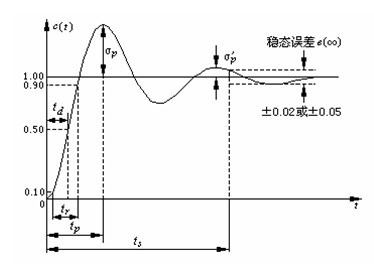
\includegraphics[scale=0.8]{danweijiyao}
\end{block}
\end{frame}
\begin{frame}
\begin{block}{}
\begin{itemize}
\item<+-> 延迟时间$t_d$:达到终值一半所需要的时间
\item<+-> 上升时间$t_r$:从终值的10\%到90\%所需要的时间
\item<+-> 峰值时间$t_p$:终值达到超调量的第一个峰值的时间
\item<+-> 最大超调量$M_p$:
\[M_p\%=\frac{c(t_p)-c(\infty)}{c(\infty)}\%\]
\end{itemize}
\end{block}
\end{frame}
\begin{frame}
\begin{block}{具有单调变化的单位阶跃响应}
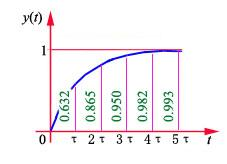
\includegraphics[scale=1.2]{onejieyaoimpulse}
\end{block}
\end{frame}
\begin{frame}{一阶系统的动态响应}
\begin{block}{一阶系统的数学模型}
\[\Phi(s)=\frac{V_2(s)}{V_1(s)}=\frac{1}{RCs+1}=\frac{1}{Ts+1}\]
其中:$T=RC$
\end{block}
\end{frame}
\begin{frame}{一阶系统的动态响应}
\begin{block}{一阶系统的单位阶跃响应}
\begin{eqnarray*}
r(t)=u(t)\\
R(s)=\frac{1}{s}\\
C(s)=\Phi(s)R(s)=\frac{1}{Ts+1}\cdot\frac{1}{s}\\
C(s)=\frac{1}{s(Ts+1)}=\frac{1}{s}-\frac{T}{Ts+1}\\
c(t)=L^{-1}[C(s)]=1-e^{-\frac{t}{T}},t\geq 0
\end{eqnarray*}
\end{block}
\end{frame}
\begin{frame}
\begin{block}{系统特性}
\begin{itemize}
\item<+-> $T$为时间常数,反映系统的惯性
\item<+-> $T$越小,系统惯性越小,系统响应越快
\item<+-> $t_s=0.3T$
\item<+-> $t_d=0.69T$
\item<+-> $t_r=2.20T$
\end{itemize}
\end{block}
\end{frame}
\begin{frame}{一阶系统的单位斜坡响应}
\begin{block}{}
\begin{eqnarray*}
C(s)=\Phi(s)R(s)=\frac{1}{Ts+1}\cdot\frac{1}{s^2}\\
C(s)=\frac{1}{s^2(Ts+1)}=\frac{1}{s^2}-\frac{T}{s}+
\frac{T^2}{Ts+1}\\
c(t)=L^{-1}[C(s)]=(t-T)+Te^{-\frac{t}{T}},t\geq 0
\end{eqnarray*}
\end{block}
\end{frame}
\begin{frame}{一阶系统的单脉冲响应}
\begin{block}{}
\begin{eqnarray*}
C(s)=\Phi(s)R(s)=\frac{1}{Ts+1}\\
c(t)=L^{-1}[C(s)]=\frac{1}{T}e^{-\frac{t}{T}},t\geq 0
\end{eqnarray*}
\end{block}
\end{frame}
%%%%%%%%%%%%%%教案头%%%%%%%%%%%%%%%%%%%%%%%%%%%%%%%
\mode<article>{

\begin{longtable}{|m{20mm}|m{20mm}|m{20mm}|m{20mm}|m{20mm}|m{28mm}|}
\caption*{\huge 教案头}\\
\hline
\endfirsthead
\multicolumn{6}{l}{(续表)}\\
\hline
\endhead
\hline
\multicolumn{6}{l}{\itshape 接下一页表格.......}\\ [2ex]
\endfoot
\hline
\endlastfoot
\centering{授课单元}&\multicolumn{3}{m{60mm}|}{\centering 2.6.4二阶系统的动态响应}&\centering{授课日期}&2014年03月13日 \\
\hline
\centering 授课地点 & \multicolumn{3}{m{60mm}|}{B6-204}&\centering 授课学时 & 2 \\
\hline
& \multicolumn{2}{m{40mm}|}{能力目标} & \multicolumn{2}{m{40mm}|}{知识目标}&素质目标 \\
\cline{2-6}
\centering 教学目标&\multicolumn{2}{m{40mm}|}{\begin{enumerate}
\item 能够分析二阶系统的动态响应
\item 能够计算二阶系统的性能指标
\end{enumerate} }&\multicolumn{2}{m{40mm}|}{\begin{enumerate}
\item 了解二阶系统的数学模型
\item 掌握二阶系统的响应分析
\end{enumerate}} & {\qquad}\\
\hline
\centering 能力训练任务或案例 &\multicolumn{5}{m{108mm}|}{ }\\
\hline
\centering 教学重点 & \multicolumn{5}{m{108mm}|}{\begin{enumerate}
\item 二阶系统的动态响应
\end{enumerate}}\\
\hline
\centering 教学难点与解决办法 &\multicolumn{5}{m{108mm}|}{\begin{enumerate}
\item 难点:二阶系统的动态响应分析
\item 解决方法:用实例进行分析讲解
\end{enumerate}}\\
\hline
\centering 德育内容 &\multicolumn{5}{m{108mm}|}{无}\\
\hline
 &教材 & \multicolumn{4}{m{88mm}|}{计算机控制原理与应用}\\
\cline{2-6}& 教学资源 &\multicolumn{4}{m{88mm}|}{PPT}\\
\cline{2-6}\centering 使用的教学材料& 主要教学仪器设备和工具等 &\multicolumn{4}{m{88mm}|}{投影机、MATLAB}\\
\cline{2-6}& 主要耗材 &\multicolumn{4}{m{88mm}|}{无}\\
\hline
\centering 教学模式 &\multicolumn{2}{m{40mm}|}{知识讲授}&\centering 教学手段 &\multicolumn{2}{m{48mm}|}{多媒体教学}\\
\hline
\centering 学生成果与过程考核方式 &\multicolumn{5}{m{108mm}|}{无}
\end{longtable}
\clearpage

%%%%%%%%%%%%%%%教学实施过程%%%%%%%%%%%%%%%%%%%%%%%%%%%%
\begin{landscape}

\begin{longtable}{|m{10mm}|m{50mm}|m{50mm}|m{50mm}|m{15mm}|}
\caption*{\huge 教学组织与实施}\\
\hline
\endfirsthead
\multicolumn{5}{l}{\small 接上页}\\
\hline
\multicolumn{1}{|c|}{步骤}&\multicolumn{1}{c|}{教学内容}&\multicolumn{1}{c|}{教师活动}&\multicolumn{1}{c|}{学生活动}&\multicolumn{1}{c|}{时间}\\
\hline
\endhead

\multicolumn{5}{r}{\small 接下页}\\
\endfoot
\hline
\endlastfoot
\multicolumn{1}{|c|}{步骤}&\multicolumn{1}{c|}{教学内容}&\multicolumn{1}{c|}{教师活动}&\multicolumn{1}{c|}{学生活动}&\multicolumn{1}{c|}{时间}\\\hline
讲解&\begin{enumerate}
\item 二阶系统的数学模型
\end{enumerate} &\begin{enumerate}
\item 讲解分析二阶系统的数学模型
\end{enumerate} &\begin{enumerate}
\item 学生倾听并记录
\end{enumerate} &15 \\\hline
讲解&\begin{enumerate}
\item 二阶系统的单位阶跃响应
\end{enumerate}
 &\begin{enumerate}
\item 通过数学分析和图示讲解二阶系统的单位阶跃响应
\end{enumerate} &\begin{enumerate}
\item 学生倾听并记录
\end{enumerate} &30 \\\hline
讲解&\begin{enumerate}
\item 典型二阶系统的动态性能指标
\end{enumerate}
&\begin{enumerate}
\item 讲解二阶系统的动态性能指标
\end{enumerate} &\begin{enumerate}
\item 学生倾听并记录
\end{enumerate} &20 \\\hline
讲解&\begin{enumerate}
\item 二阶系统的单位脉冲响应
\end{enumerate}
 &\begin{enumerate}
\item 讲解阶系统的单位阶跃响应分析
\end{enumerate} &\begin{enumerate}
\item 学生记录笔记
\end{enumerate} &20 \\\hline
总结&
\begin{enumerate}
\item 二阶系统的动态响应
\end{enumerate}
 &\begin{enumerate}
\item 总结二阶系统的动态响应
\end{enumerate} &\begin{enumerate}
\item 学生记录笔记
\end{enumerate} &5 \\\hline
\centering 本次课总结(评价)&总结本课程内容 &进行知识总结 &学生倾听 &5 \\\hline
\centering 学生学习笔记或工单等检查情况&\multicolumn{4}{m{165mm}|}{\quad}\\\hline
\centering 课后作业&\multicolumn{4}{m{165mm}|}{2-19,2-20,2-21}\\\hline
\centering 教学体会&\multicolumn{4}{m{165mm}|}{\quad}\\
\end{longtable}

\end{landscape}
\clearpage
%%%%%%%%%%%%%%%%%%%%板书设计%%%%%%%%%%%%%%%%%%%%%%%%%%
\begin{center}
{\huge 板书设计}
\end{center}
}
\mode<presentation>{ \section{控制系统的时域分析}
 \subsection{二阶系统的动态响应}}
 \begin{frame}{二阶系统的数学模型}
 \begin{block}{}
 \begin{itemize}
 \item<+-> RLC网络的二阶微分方程:
 \[\frac{d^2c(t)}{dt^2}+\frac{R}{L}\frac{dc(t)}{dt}+\frac{1}{LC}c(t)=\frac{1}{LC}r(t)\]
 \item<+-> 典型形式为:
 \[\frac{d^2c(t)}{dt^2}+2\zeta\omega_n\frac{dc(t)}{dt}+\omega_n^2=\omega_n^2r(t)\]
 \end{itemize}
 \end{block}
 \end{frame}
 
 \begin{frame}
 \begin{block}{}
 \begin{itemize}
 \item<+-> 其中:
 \[\omega_n=\frac{1}{\sqrt{LC}}\]
 \[2\zeta\omega_n=\frac{R}{L}\]
 \[\zeta=\frac{R}{2}\sqrt{\frac{C}{L}}\]
\end{itemize}  
\end{block}
\end{frame}

\begin{frame}
\begin{block}{}
\begin{itemize}
\item<+-> 进行拉氏变换得:
\[s^2C(s)+2\zeta\omega_nsC(s)+\omega_n^2C(s)=\omega_n^2R(s)\]
\item<+-> 系统开环传递函数为:
\[G_o(s)=\frac{C(s)}{E(s)}=\frac{\omega^2_n}{s(s+2\zeta\omega_n)}\]
\end{itemize}
\end{block}
\end{frame}
\begin{frame}
\begin{block}{}
\begin{itemize}
\item<+-> 系统闭环传递函数为:
\[\Phi(s)=\frac{C(s)}{R(s)}=\frac{\omega_n^2}{s^2+2\zeta\omega_ns+\omega_n^2}\]
\item<+-> 系统特征方程为:
\[s^2+2\zeta\omega_ns+\omega_n^2=0\]
\end{itemize}
\end{block}
\end{frame}
\begin{frame}
\uncover<+->{\begin{block}{}
特征根为:
\[s_{1,2}=-\zeta\omega_n\pm\omega_n\sqrt{\zeta^2-1}\]
\end{block}}
\uncover<+->{\begin{block}{}
系统的特征取决于$\zeta$和$\omega_n$两个参数
\end{block}}
\end{frame}

\begin{frame}{二阶系统的单位阶跃响应}
\begin{block}{}
\begin{itemize}
\item<+-> 单位阶跃函数的拉氏变换为:
\[R(s)=\frac{1}{s}\]
\item<+-> 系统输入的拉氏变换为:
\[C(s)=\Phi(s)R(s)=\frac{\omega_n^2}{s^2+2\zeta\omega_ns+\omega_n^2}\cdot\frac{1}{s}\]
\end{itemize}
\end{block}
\end{frame}
\begin{frame}
\begin{block}{当$\zeta=0$时}
\begin{itemize}
\item<+-> 则:
\[C(s)=\frac{\omega_n^2}{s^2+\omega_n^2}\cdot\frac{1}{s}\]
\item<+-> 展开得:
\[C(s)=\frac{\omega_n^2}{s(s^2+\omega_n^2)}=\frac{1}{s}-\frac{s}{s^2+\omega_n^2}\]
\end{itemize}
\end{block}
\end{frame}
\begin{frame}
\begin{block}{}
\begin{itemize}
\item<+-> 拉氏逆变换得:
\[c(t)=1-\cos\omega_nt\]
\item<+-> 系统响应曲线:

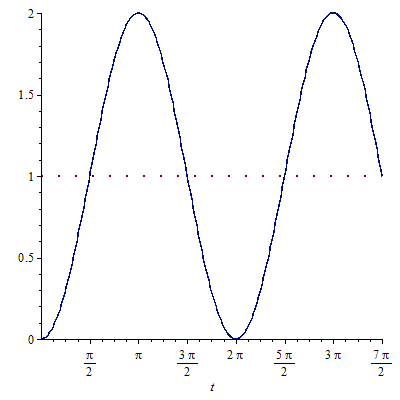
\includegraphics[scale=0.25]{wuzuni.png}
\end{itemize}
\end{block}
\end{frame}
\begin{frame}
\begin{block}{当$0<\zeta<1$时}
\begin{itemize}
\item<+-> 系统特征方程根为:
\[s_1=-\zeta\omega_n+j\omega_n\sqrt{1-\zeta^2}=-\zeta\omega_n+j\omega_d\]
\[s_2=-\zeta\omega_n-j\omega_n\sqrt{1-\zeta^2}=-\zeta\omega_n-j\omega_d\]
\end{itemize}
其中:$\omega_d=\omega_n\sqrt{1-\zeta^2}$
\end{block}
\end{frame}
\begin{frame}
\begin{block}{}
\begin{itemize}
\item<+-> 特征方程可写为:
\begin{eqnarray*}
s^2+2\zeta\omega_ns+\omega_n^2\\
=(s+\zeta\omega_n-j\omega_d)(s+\zeta\omega_n+j\omega_d)
\end{eqnarray*}
\end{itemize}
\end{block}
\end{frame}
\begin{frame}
\begin{block}{}
系统输出$C(s)$为:
\begin{eqnarray*}
C(s)=\Phi(s)R(s)=\frac{\omega_n^2}{s^2+2\zeta\omega_ns+\omega_n^2}\frac{1}{s}\\
=\frac{1}{s}-\frac{s+\zeta\omega_n}{(s+\zeta\omega_n)^2+\omega_d^2}-\frac{\zeta\omega_n}{(s+\zeta\omega_n)^2+\omega_d^2}
\end{eqnarray*}
\end{block}
\end{frame}
\begin{frame}
\begin{block}{}
\begin{itemize}
\item<+-> 拉氏逆变换为:
\begin{eqnarray*}
c(t)=L^{-1}[C(s)]\\
=1-e^{-\zeta\omega_nt}\frac{1}{\sqrt{1-\zeta^2}}\sin(\omega_dt+\varphi),t\geq 0
\end{eqnarray*}
\end{itemize}
\end{block}
\end{frame}
\begin{frame}
\begin{block}{当$\zeta=1$时}
\begin{itemize}
\item<+-> 系统的特征方程为:
\[s^2+2\zeta\omega_ns+\omega_n^2=s^2+2\omega_n+\omega_n^2=(s+\omega_n)^2\]
\item<+-> 系统输出为:
\[C(s)=\Phi(s)R(s)=\frac{\omega_n^2}{(s+\omega_n)^2}\cdot\frac{1}{s}\]
\end{itemize}
\end{block}
\end{frame}
\begin{frame}
\begin{block}{}
\begin{itemize}
\item<+-> 展开得:
\begin{eqnarray*}
C(s)=\frac{\omega_n^2}{s(s+\omega_n)^2}\\
=\frac{1}{s}-\frac{1}{s+\omega_n}-\frac{\omega_n}{(s+\omega_n)^2}
\end{eqnarray*} 
\item<+-> 拉氏逆变换得:
\[c(t)=1-e^{-\omega_nt}-e^{\omega_nt}\omega_nt,t\geq 0\]
\end{itemize}
\end{block}
\end{frame}
\endinput
%%%%%%%%%%%%%%教案头%%%%%%%%%%%%%%%%%%%%%%%%%%%%%%%
\mode<article>{

\begin{longtable}{|m{20mm}|m{20mm}|m{20mm}|m{20mm}|m{20mm}|m{28mm}|}
\caption*{\huge 教案头}\\
\hline
\endfirsthead
\multicolumn{6}{l}{(续表)}\\
\hline
\endhead
\hline
\multicolumn{6}{l}{\itshape 接下一页表格.......}\\ [2ex]
\endfoot
\hline
\endlastfoot
\centering{授课单元}&\multicolumn{3}{m{60mm}|}{\centering 2.6.5高阶系统分析2.6.6稳态误差分析}&\centering{授课日期}&2014年04月18日 \\
\hline
\centering 授课地点 & \multicolumn{3}{m{60mm}|}{B6-204}&\centering 授课学时 & 2 \\
\hline
& \multicolumn{2}{m{40mm}|}{能力目标} & \multicolumn{2}{m{40mm}|}{知识目标}&素质目标 \\
\cline{2-6}
\centering 教学目标&\multicolumn{2}{m{40mm}|}{\begin{enumerate}
\item 能够分析系统的稳态误差
\end{enumerate} }&\multicolumn{2}{m{40mm}|}{\begin{enumerate}
\item 了解高附系统的分析方法
\item 掌握系统的稳态误差分析
\end{enumerate}} & {\qquad}\\
\hline
\centering 能力训练任务或案例 &\multicolumn{5}{m{108mm}|}{ }\\
\hline
\centering 教学重点 & \multicolumn{5}{m{108mm}|}{\begin{enumerate}
\item 系统的稳态误差分析
\end{enumerate}}\\
\hline
\centering 教学难点与解决办法 &\multicolumn{5}{m{108mm}|}{\begin{enumerate}
\item 难点:系统的稳态误差分析
\item 解决方法:数学推理加实例讲解
\end{enumerate}}\\
\hline
\centering 德育内容 &\multicolumn{5}{m{108mm}|}{无}\\
\hline
 &教材 & \multicolumn{4}{m{88mm}|}{计算机控制原理与应用}\\
\cline{2-6}& 教学资源 &\multicolumn{4}{m{88mm}|}{PPT}\\
\cline{2-6}\centering 使用的教学材料& 主要教学仪器设备和工具等 &\multicolumn{4}{m{88mm}|}{投影机、MATLAB}\\
\cline{2-6}& 主要耗材 &\multicolumn{4}{m{88mm}|}{无}\\
\hline
\centering 教学模式 &\multicolumn{2}{m{40mm}|}{知识讲授}&\centering 教学手段 &\multicolumn{2}{m{48mm}|}{多媒体教学}\\
\hline
\centering 学生成果与过程考核方式 &\multicolumn{5}{m{108mm}|}{无}
\end{longtable}
\clearpage

%%%%%%%%%%%%%%%教学实施过程%%%%%%%%%%%%%%%%%%%%%%%%%%%%
\begin{landscape}

\begin{longtable}{|m{10mm}|m{50mm}|m{50mm}|m{50mm}|m{15mm}|}
\caption*{\huge 教学组织与实施}\\
\hline
\endfirsthead
\multicolumn{5}{l}{\small 接上页}\\
\hline
\multicolumn{1}{|c|}{步骤}&\multicolumn{1}{c|}{教学内容}&\multicolumn{1}{c|}{教师活动}&\multicolumn{1}{c|}{学生活动}&\multicolumn{1}{c|}{时间}\\
\hline
\endhead

\multicolumn{5}{r}{\small 接下页}\\
\endfoot
\hline
\endlastfoot
\multicolumn{1}{|c|}{步骤}&\multicolumn{1}{c|}{教学内容}&\multicolumn{1}{c|}{教师活动}&\multicolumn{1}{c|}{学生活动}&\multicolumn{1}{c|}{时间}\\\hline
讲解&\begin{enumerate}
\item 高阶系统的单位阶跃响应
\end{enumerate} &\begin{enumerate}
\item 讲解高阶系统的单位阶跃响应
\end{enumerate} &\begin{enumerate}
\item 学生倾听并记录
\end{enumerate} &30 \\\hline
讲解&\begin{enumerate}
\item 高阶系统分析
\end{enumerate}
 &\begin{enumerate}
\item 讲解高阶系统分析方法
\end{enumerate} &\begin{enumerate}
\item 学生倾听并记录
\end{enumerate} &15 \\\hline
讲解&\begin{enumerate}
\item 稳态误差分析
\end{enumerate}
&\begin{enumerate}
\item 讲解系统稳态分析
\end{enumerate} &\begin{enumerate}
\item 学生倾听并记录
\end{enumerate} &20 \\\hline
讲解&\begin{enumerate}
\item 稳态误差分析实例
\end{enumerate}
 &\begin{enumerate}
\item 讲解稳态误差分析实例
\end{enumerate} &\begin{enumerate}
\item 学生记录笔记
\end{enumerate} &20 \\\hline

\centering 本次课总结(评价)&总结本课程内容 &进行知识总结 &学生倾听 &5 \\\hline
\centering 学生学习笔记或工单等检查情况&\multicolumn{4}{m{165mm}|}{\quad}\\\hline
\centering 课后作业&\multicolumn{4}{m{165mm}|}{2-19,2-20,2-21}\\\hline
\centering 教学体会&\multicolumn{4}{m{165mm}|}{\quad}\\
\end{longtable}

\end{landscape}
\clearpage
%%%%%%%%%%%%%%%%%%%%板书设计%%%%%%%%%%%%%%%%%%%%%%%%%%
\begin{center}
{\huge 板书设计}
\end{center}
}
\mode<presentation>{ \section{高阶系统分析}
 \subsection{高阶系统分析}}
 \begin{frame}{高阶系统的单位阶跃响应}
 \begin{block}{高阶闭环传递函数}
 \begin{eqnarray*}
 \Phi(s)&=&\frac{C(s)}{R(s)}=\frac{B(s)}{A(s)}\\
 &=&\frac{b_0s^m+b_1s^{m-1}+\cdots +b_{m-1}s+b_m}{s^n+a_1s^{n-1}+\cdots +a_{n-1}s+a_n}
 \end{eqnarray*}
 其中:$B(s)$为分子多项式,$A(s)$为分母多项式
 \end{block}
 \end{frame}
 
 \begin{frame}
 \begin{block}{极点、零点形式}
 \begin{eqnarray*}
 \Phi(s)&=&\frac{C(s)}{R(s)}=\frac{B(s)}{A(s)}\\
&=&\frac{K\prod\limits_{i=1}^m(s-z_i)}{\prod\limits_{j=1}^{n_1}(s-p_j)\prod\limits_{i=1}^{n_2}(s^2+2\zeta_l\omega_ls+\omega_l^2)}
\end{eqnarray*}  
\end{block}
\end{frame}

\begin{frame}
\begin{block}{单位阶跃输出部分展开式}
\begin{eqnarray*}
C(s)=\frac{K\prod\limits_{i=1}^m(s-z_i)}{s[\prod\limits_{j=1}^{n_1}(s-p_j)\prod\limits_{i=1}^{n_2}(s^2+2\zeta_l\omega_ls+\omega_l^2)]}\\
=\frac{a_0}{s}+\sum_{j=1}^{n_1}\frac{a_j}{s-p_j}+\sum_{l=1}^{n_2}\frac{\beta_ls+r_l}{(s-p_{1l})(s-p_{2l})}
\end{eqnarray*}
其中:$a_0,a_j,\beta_l,r_l$为待定系数
\end{block}
\end{frame}
\begin{frame}
待定系统求法:
\[a_0=[sC(s)]\mid_{s=0}\]
\[a_j=[(s-p_j)C(s)]\mid_{s=p_j},j=1,2,\cdots ,n\]
\[\beta_ls+r_l \]
\[=[(s-p_{1l})(s-P_{2l}C(s)]\mid_{s=p_{1l}(or s=p_{2l})},\]
\[l=1,2,\cdots ,n\]
\end{frame}
\begin{frame}
\begin{block}{拉氏变换}
\begin{eqnarray*}
c(t)&=&L^{-1}[C(s)]\\
&=&a_0+\sum_{j=1}^{n_1}a_je^{p_jt}+\\
&&\sum_{l=1}^{n_1}\beta_le^{-\zeta_l\omega_lt}\cos\omega_l\sqrt{1-\zeta^2_l}t+\\
&&\sum_{l=1}^{n_2}\frac{r_l-\beta_l\zeta_l\omega_l}{\omega_l\sqrt{1-\zeta_l^2}}e^{-\zeta_l\omega_lt}\sin\omega_l\sqrt{1-\zeta_l^2}t
\end{eqnarray*}
\end{block}
\end{frame}

\begin{frame}{高阶系统分析}
\begin{block}{}
\begin{itemize}
\item<+-> 位于左半s平面,系统稳定
\item<+-> 若系统稳定:离虚轴越远,则指数项衰减走越快、
\item<+-> 实际中,常用根轨迹法、频率法等
\end{itemize}
\end{block}
\end{frame}
\begin{frame}{稳态误差分析}
\begin{block}{系统开环传递函数}
\begin{eqnarray*}
G_o(s)=\frac{K(1+\tau_1s)(1+\tau_2s)\cdots(1+\tau_ms}{s^q(1+T_1s)(1+T_2s)\cdots(1+T_{n-q}s)}
\end{eqnarray*}
其中:$K$为开环增益;\\
$\tau_1,\tau_2,\cdots,\tau_m$和$T_1,T_2,\cdots,T_n$为时间常数;\\
$q$为开环系统在$s$平面坐标原点上重极点数
\end{block}
\end{frame}
\begin{frame}
\begin{block}{稳态误差}
\begin{itemize}
\item<+-> 闭环传递函数为:
\[\Phi(s)=\frac{C(s)}{R(s)}=\frac{G(s)}{1+H(s)G(s)}\]
\item<+-> 则开环为:
\[G_o(s)=G(s)H(s)\]
\end{itemize}
\end{block}
\end{frame}
\begin{frame}
\begin{block}{}
\begin{itemize}
\item<+-> 误差信息$e(t)$为:
\[e(t)=r(t)-b(t)\]
\item<+-> 拉氏变换为:
\[E(s)=R(s)-B(s)=R(s)-H(s)C(s)\]
\end{itemize}
\end{block}
\end{frame}
\begin{frame}
\begin{block}{误差传递函数为}
\begin{eqnarray*}
\Phi_E(s)&=&\frac{E(s)}{R(s)}=\frac{1}{1+H(s)G(s)}\\
E(s)&=&\Phi_E(s)R(s)\\
&=&\frac{1}{1+H(s)G(s)}R(s)\\
&=&\frac{1}{1+G_o(s)}R(s)
\end{eqnarray*}
\end{block}
\end{frame}
\begin{frame}
\begin{block}{系统稳态误差}
\begin{eqnarray*}
e_{ss}&=&\lim_{s\rightarrow \infty}e(t)=\lim_{s\rightarrow 0}sE(s)\\
&=&\lim_{s\rightarrow 0}\frac{sR(s)}{1+H(s)R(s)}\\
&=&\lim_{s\rightarrow 0}\frac{sR(s)}{1+G_o(s)}
\end{eqnarray*}
\end{block}
\end{frame}
\begin{frame}
\begin{block}{阶跃输入的稳态误差}
\begin{eqnarray*}
e_{ss}(step)&=&\lim\limits_{s\rightarrow 0}\frac{s}{1+G_o(s)}\frac{R_0}{s}\\
&=&\lim\limits_{s\rightarrow 0}\frac{R_0}{1+G_o(s)}\\
&=&\lim\limits_{s\rightarrow 0}\frac{R_0}{1+K_p}\\
K_p&=&\lim\limits_{s\rightarrow 0}G_o(s)=\lim\limits_{s\rightarrow 0}H(s)G(s)
\end{eqnarray*}
\end{block}
\end{frame}
\begin{frame}
\begin{block}{斜坡输入时的稳态误差}
\begin{eqnarray*}
e_{ss}(ramp)&=&\lim\limits_{s\rightarrow 0}\frac{s}{1+G_o(s)}\frac{R_0}{s^2}\\
&=&\lim\limits_{s\rightarrow 0}\frac{R_0}{sG_o(s)}\\
&=&\frac{R_0}{K_V}\\
K_V&=&\lim\limits_{s\rightarrow 0}sG_o(s)=\lim\limits_{s\rightarrow 0}sH(s)G(s)
\end{eqnarray*}
\end{block}
\end{frame}
\begin{frame}
\begin{block}{抛物线输入时的稳态误差}
\begin{eqnarray*}
&&e_{ss}(parabolic)=\lim\limits_{s\rightarrow 0}\frac{s}{1+G_o(s)}\frac{R_0}{s^3}\\
&=&\lim\limits_{s\rightarrow 0}\frac{R_0}{s^2G_o(s)}\\
&=&\frac{R_0}{K_a}\\
K_a&=&\lim\limits_{s\rightarrow 0}s^2G_o(s)=\lim\limits_{s\rightarrow 0}s^2H(s)G(s)
\end{eqnarray*}
\end{block}
\end{frame}
\endinput
%%%%%%%%%%%%%%教案头%%%%%%%%%%%%%%%%%%%%%%%%%%%%%%%
\mode<article>{

\begin{longtable}{|m{20mm}|m{20mm}|m{20mm}|m{20mm}|m{20mm}|m{28mm}|}
\caption*{\huge 教案头}\\
\hline
\endfirsthead
\multicolumn{6}{l}{(续表)}\\
\hline
\endhead
\hline
\multicolumn{6}{l}{\itshape 接下一页表格.......}\\ [2ex]
\endfoot
\hline
\endlastfoot
\centering{授课单元}&\multicolumn{3}{m{60mm}|}{\centering 2.6.8稳定性分析}&\centering{授课日期}&2014年04月25日 \\
\hline
\centering 授课地点 & \multicolumn{3}{m{60mm}|}{B6-204}&\centering 授课学时 & 2 \\
\hline
& \multicolumn{2}{m{40mm}|}{能力目标} & \multicolumn{2}{m{40mm}|}{知识目标}&素质目标 \\
\cline{2-6}
\centering 教学目标&\multicolumn{2}{m{40mm}|}{\begin{enumerate}
\item 能够分析系统的稳定性
\end{enumerate} }&\multicolumn{2}{m{40mm}|}{\begin{enumerate}
\item 了解系统的极点、零点和稳定性的概念
\item 掌握劳斯稳定性判据
\end{enumerate}} & {\qquad}\\
\hline
\centering 能力训练任务或案例 &\multicolumn{5}{m{108mm}|}{ }\\
\hline
\centering 教学重点 & \multicolumn{5}{m{108mm}|}{\begin{enumerate}
\item 劳斯稳定性判据
\end{enumerate}}\\
\hline
\centering 教学难点与解决办法 &\multicolumn{5}{m{108mm}|}{\begin{enumerate}
\item 难点:劳斯稳定性判据
\item 解决方法:实例讲解
\end{enumerate}}\\
\hline
\centering 德育内容 &\multicolumn{5}{m{108mm}|}{无}\\
\hline
 &教材 & \multicolumn{4}{m{88mm}|}{计算机控制原理与应用}\\
\cline{2-6}& 教学资源 &\multicolumn{4}{m{88mm}|}{PPT}\\
\cline{2-6}\centering 使用的教学材料& 主要教学仪器设备和工具等 &\multicolumn{4}{m{88mm}|}{投影机、MATLAB}\\
\cline{2-6}& 主要耗材 &\multicolumn{4}{m{88mm}|}{无}\\
\hline
\centering 教学模式 &\multicolumn{2}{m{40mm}|}{知识讲授}&\centering 教学手段 &\multicolumn{2}{m{48mm}|}{多媒体教学}\\
\hline
\centering 学生成果与过程考核方式 &\multicolumn{5}{m{108mm}|}{无}
\end{longtable}
\clearpage

%%%%%%%%%%%%%%%教学实施过程%%%%%%%%%%%%%%%%%%%%%%%%%%%%
\begin{landscape}

\begin{longtable}{|m{10mm}|m{50mm}|m{50mm}|m{50mm}|m{15mm}|}
\caption*{\huge 教学组织与实施}\\
\hline
\endfirsthead
\multicolumn{5}{l}{\small 接上页}\\
\hline
\multicolumn{1}{|c|}{步骤}&\multicolumn{1}{c|}{教学内容}&\multicolumn{1}{c|}{教师活动}&\multicolumn{1}{c|}{学生活动}&\multicolumn{1}{c|}{时间}\\
\hline
\endhead

\multicolumn{5}{r}{\small 接下页}\\
\endfoot
\hline
\endlastfoot
\multicolumn{1}{|c|}{步骤}&\multicolumn{1}{c|}{教学内容}&\multicolumn{1}{c|}{教师活动}&\multicolumn{1}{c|}{学生活动}&\multicolumn{1}{c|}{时间}\\\hline
讲解&\begin{enumerate}
\item 极点、零点和稳定性的概念
\end{enumerate} &\begin{enumerate}
\item 讲解极点、零点和稳定性的概念
\end{enumerate} &\begin{enumerate}
\item 学生倾听并记录
\end{enumerate} &15 \\\hline
讲解&\begin{enumerate}
\item 稳定性判定的数学理论
\end{enumerate}
 &\begin{enumerate}
\item 讲解稳定性判定的数学理论
\end{enumerate} &\begin{enumerate}
\item 学生倾听并记录
\end{enumerate} &30 \\\hline
讲解&\begin{enumerate}
\item 劳斯稳定性判据
\end{enumerate}
&\begin{enumerate}
\item 讲解劳斯稳定性判据
\end{enumerate} &\begin{enumerate}
\item 学生倾听并记录
\end{enumerate} &20 \\\hline
讲解&\begin{enumerate}
\item 劳斯稳定性判据的应用实例
\end{enumerate}
 &\begin{enumerate}
\item 讲解劳斯稳定性判据的应用实例
\end{enumerate} &\begin{enumerate}
\item 学生记录笔记
\end{enumerate} &20 \\\hline

\centering 本次课总结(评价)&总结本课程内容 &进行知识总结 &学生倾听 &5 \\\hline
\centering 学生学习笔记或工单等检查情况&\multicolumn{4}{m{165mm}|}{\quad}\\\hline
\centering 课后作业&\multicolumn{4}{m{165mm}|}{2-28,2-29}\\\hline
\centering 教学体会&\multicolumn{4}{m{165mm}|}{\quad}\\
\end{longtable}

\end{landscape}
\clearpage
%%%%%%%%%%%%%%%%%%%%板书设计%%%%%%%%%%%%%%%%%%%%%%%%%%
\begin{center}
{\huge 板书设计}
\end{center}
}
\mode<presentation>{ \section{稳定性分析}
 \subsection{稳定性分析}}
 \begin{frame}{极点、零点和稳定性}
 \begin{block}{$n$阶传递函数的因子形式}
 \begin{eqnarray*}
 \Phi(s)&=&\frac{C(s)}{R(s)}\\
 &=&\frac{K\prod\limits_{i=1}^m(s-z_i)}{\prod\limits_{j=1}^{n_1}(s-p_j)\prod\limits_{l=1}^{n_2}(s^2+2\zeta_l\omega_ls+\omega_l^2)}
 \end{eqnarray*}
 \end{block}
 \end{frame}
 
 \begin{frame}
 \begin{block}{极点、零点的定义}
 设:
 \begin{eqnarray*}
 &&s^2+2\zeta_l\omega_l+\omega_l^2=(s-p_{1l})(s-p_{2l})\\
 &&s_{1l,2l}=-\zeta_l\omega_l\pm j\omega_l\sqrt{1-\zeta_l^2}\\
 &&l=1,2,\cdots ,n_2
\end{eqnarray*}
\begin{itemize}
\item $z_1,z_2,\cdots,z_m$称为零点
\item $p_{11},p_{12},\cdots,p_{1n_2},p_{21},p_{22},\cdots,p_{2n_2}$和\\
$p_1,p_2,\cdots,p_{n_1}$称为极点
\end{itemize}  
\end{block}
\end{frame}

\begin{frame}
\begin{block}{稳定性}
\begin{itemize}
\item 稳定系统
$\lim\limits_{t\rightarrow \infty}g(t)=0$
\item 不稳定系统
$\lim\limits_{t\rightarrow \infty}g(t)=\infty$
\item 临界稳定系统
$\lim\limits_{t\rightarrow \infty}g(t)=P$
\end{itemize}
\end{block}
\end{frame}
\begin{frame}
\begin{block}{单位脉冲输出部分展开式}
\begin{eqnarray*}
\Phi(s)=\frac{K\prod\limits_{i=1}^m(s-z_i)}{\prod\limits_{j=1}^{n_1}(s-p_j)\prod\limits_{i=1}^{n_2}(s^2+2\zeta_l\omega_ls+\omega_l^2)}\\
=\sum_{j=1}^{n_1}\frac{a_j}{s-p_j}+\sum_{l=1}^{n_2}\frac{\beta_ls+r_l}{(s-p_{1l})(s-p_{2l})}
\end{eqnarray*}
其中:$a_0,a_j,\beta_l,r_l$为待定系数
\end{block}
\end{frame}

\begin{frame}
\begin{block}{拉氏变换}
\begin{eqnarray*}
g(t)&=&L^{-1}[C(s)]=L^{-1}[\Phi(s)]\\
&=&\sum_{j=1}^{n_1}a_je^{p_jt}+\\
&&\sum_{l=1}^{n_1}\beta_le^{-\zeta_l\omega_lt}\cos\omega_l\sqrt{1-\zeta^2_l}t+\\
&&\sum_{l=1}^{n_2}\frac{r_l-\beta_l\zeta_l\omega_l}{\omega_l\sqrt{1-\zeta_l^2}}e^{-\zeta_l\omega_lt}\sin\omega_l\sqrt{1-\zeta_l^2}t
\end{eqnarray*}
\end{block}
\end{frame}

\begin{frame}{劳斯稳定性判据}
\begin{block}{$n$阶线性定常系统的特征方程}
\[a_0s^n+a_1+s^{n-1}+\cdots+a_{n-1}s+a_n=0\]
\end{block}
\end{frame}
\begin{frame}
\begin{block}{劳斯表}
\begin{equation*}
\begin{array}{cccccc}
s^n&a_0&a_2&a_4&a_6&\cdots\\
s^{n-1}&a_1&a_3&a_5&a_7&\cdots\\
S^{n-2}&T_{3,1}&T_{3,2}&T_{3,3}&T_{3,4}&\cdots\\
S^{n-3}&T_{4,1}&T_{4,2}&T_{4,3}&T_{4,4}&\cdots\\
\cdots&\cdots&\cdots&\cdots&\cdots&\cdots\\
s^2&T_{n-1,1}&T_{n-1,2}\\
s^1&T_{n,1}\\
s^0&T_{n+1,1}
\end{array}
\end{equation*}
\end{block}
\end{frame}

\begin{frame}
\begin{block}{}
\begin{eqnarray*}
T_{3,1}=-\frac{\left|\begin{array}{cc}
a_0&a_2\\
a_1&a_3
\end{array}\right|}{a_1}=\frac{a_1a_2-a_0a_3}{a_1}\\
T_{3,2}=-\frac{\left|\begin{array}{cc}
a_0&a_4\\
a_1&a_5
\end{array}\right|}{a_1}=\frac{a_1a_4-a_0a_5}{a_1}\\
T_{3,3}=-\frac{\left|\begin{array}{cc}
a_0&a_6\\
a_1&a_7
\end{array}\right|}{a_1}=\frac{a_1a_6-a_0a_7}{a_1}
\end{eqnarray*}
\end{block}
\end{frame}
\begin{frame}
\begin{block}{}
\begin{eqnarray*}
T_{4,1}=-\frac{\left|\begin{array}{cc}
a_1&a_3\\
T_{3,1}&T_{3,2}
\end{array}\right|}{T_{3,1}}=\frac{T_{3,1}a_3-T_{3,2}a_1}{T_{3,1}}\\
T_{4,2}=-\frac{\left|\begin{array}{cc}
a_1&a_5\\
T_{3,1}&T_{3,3}
\end{array}\right|}{T_{3,1}}=\frac{T_{3,1}a_5-a_1T_{3,3}}{T_{3,1}}\\
\vdots
\end{eqnarray*}
\end{block}
\end{frame}

\begin{frame}
\begin{block}{}
\begin{eqnarray*}
T_{5,1}=-\frac{\left|\begin{array}{cc}
T_{3,1}&T_{3,2}\\
T_{4,1}&T_{4,2}
\end{array}\right|}{T_{4,1}}=\frac{T_{4,1}T_{3,2}-T_{3,1}T_{4,2}}{T_{4,1}}\\
T_{5,2}=-\frac{\left|\begin{array}{cc}
T_{3,1}&T_{3,3}\\
T_{4,1}&T_{4,3}
\end{array}\right|}{T_{4,1}}=\frac{T_{4,1}T_{3,3}-T_{3,1}T_{4,3}}{T_{4,1}}\\
T_{5,3}=-\frac{\left|\begin{array}{cc}
T_{3,1}&T_{3,4}\\
T_{4,1}&T_{4,4}
\end{array}\right|}{T_{4,1}}=\frac{T_{4,1}T_{3,4}-T_{3,1}T_{4,4}}{T_{4,1}}
\end{eqnarray*}
\end{block}
\end{frame}

\endinput
%%%%%%%%%%%%%%教案头%%%%%%%%%%%%%%%%%%%%%%%%%%%%%%%
\mode<article>{

\begin{longtable}{|m{20mm}|m{20mm}|m{20mm}|m{20mm}|m{20mm}|m{28mm}|}
\caption*{\huge 教案头}\\
\hline
\endfirsthead
\multicolumn{6}{l}{(续表)}\\
\hline
\endhead
\hline
\multicolumn{6}{l}{\itshape 接下一页表格.......}\\ [2ex]
\endfoot
\hline
\endlastfoot
\centering{授课单元}&\multicolumn{3}{m{60mm}|}{\centering 2.7根轨迹}&\centering{授课日期}&2014年04月28日 \\
\hline
\centering 授课地点 & \multicolumn{3}{m{60mm}|}{B6-204}&\centering 授课学时 & 2 \\
\hline
& \multicolumn{2}{m{40mm}|}{能力目标} & \multicolumn{2}{m{40mm}|}{知识目标}&素质目标 \\
\cline{2-6}
\centering 教学目标&\multicolumn{2}{m{40mm}|}{\begin{enumerate}
\item 能够分析系统的根轨迹
\end{enumerate} }&\multicolumn{2}{m{40mm}|}{\begin{enumerate}
\item 掌握根轨迹法
\item 掌握根轨迹的绘制要点
\end{enumerate}} & {\qquad}\\
\hline
\centering 能力训练任务或案例 &\multicolumn{5}{m{108mm}|}{ }\\
\hline
\centering 教学重点 & \multicolumn{5}{m{108mm}|}{\begin{enumerate}
\item 根轨迹的绘制
\end{enumerate}}\\
\hline
\centering 教学难点与解决办法 &\multicolumn{5}{m{108mm}|}{\begin{enumerate}
\item 难点:根轨迹的绘制
\item 解决方法:实例讲解
\end{enumerate}}\\
\hline
\centering 德育内容 &\multicolumn{5}{m{108mm}|}{无}\\
\hline
 &教材 & \multicolumn{4}{m{88mm}|}{计算机控制原理与应用}\\
\cline{2-6}& 教学资源 &\multicolumn{4}{m{88mm}|}{PPT}\\
\cline{2-6}\centering 使用的教学材料& 主要教学仪器设备和工具等 &\multicolumn{4}{m{88mm}|}{投影机、MATLAB}\\
\cline{2-6}& 主要耗材 &\multicolumn{4}{m{88mm}|}{无}\\
\hline
\centering 教学模式 &\multicolumn{2}{m{40mm}|}{知识讲授}&\centering 教学手段 &\multicolumn{2}{m{48mm}|}{多媒体教学}\\
\hline
\centering 学生成果与过程考核方式 &\multicolumn{5}{m{108mm}|}{无}
\end{longtable}
\clearpage

%%%%%%%%%%%%%%%教学实施过程%%%%%%%%%%%%%%%%%%%%%%%%%%%%
\begin{landscape}

\begin{longtable}{|m{10mm}|m{50mm}|m{50mm}|m{50mm}|m{15mm}|}
\caption*{\huge 教学组织与实施}\\
\hline
\endfirsthead
\multicolumn{5}{l}{\small 接上页}\\
\hline
\multicolumn{1}{|c|}{步骤}&\multicolumn{1}{c|}{教学内容}&\multicolumn{1}{c|}{教师活动}&\multicolumn{1}{c|}{学生活动}&\multicolumn{1}{c|}{时间}\\
\hline
\endhead

\multicolumn{5}{r}{\small 接下页}\\
\endfoot
\hline
\endlastfoot
\multicolumn{1}{|c|}{步骤}&\multicolumn{1}{c|}{教学内容}&\multicolumn{1}{c|}{教师活动}&\multicolumn{1}{c|}{学生活动}&\multicolumn{1}{c|}{时间}\\\hline
讲解&\begin{enumerate}
\item 根轨迹法
\end{enumerate} &\begin{enumerate}
\item 讲解讲解根轨迹法的理论
\end{enumerate} &\begin{enumerate}
\item 学生倾听并记录
\end{enumerate} &20 \\\hline
讲解&\begin{enumerate}
\item 根轨迹图的绘制
\end{enumerate}
 &\begin{enumerate}
\item 讲解根轨迹图的绘制方法
\end{enumerate} &\begin{enumerate}
\item 学生倾听并记录
\end{enumerate} &25 \\\hline
讲解&\begin{enumerate}
\item 用MatLab绘制根轨迹图
\end{enumerate}
&\begin{enumerate}
\item 讲解用MatLab绘制根轨迹图
\end{enumerate} &\begin{enumerate}
\item 学生倾听并记录
\end{enumerate} &10 \\\hline
讲解&\begin{enumerate}
\item MatLab根轨迹图绘制实践
\end{enumerate}
 &\begin{enumerate}
\item 指导学生用MatLab绘制根轨迹图
\end{enumerate} &\begin{enumerate}
\item 学生用MatLab绘制根轨迹图
\end{enumerate} &30 \\\hline

\centering 本次课总结(评价)&总结本课程内容 &进行知识总结 &学生倾听 &5 \\\hline
\centering 学生学习笔记或工单等检查情况&\multicolumn{4}{m{165mm}|}{\quad}\\\hline
\centering 课后作业&\multicolumn{4}{m{165mm}|}{2-28,2-29}\\\hline
\centering 教学体会&\multicolumn{4}{m{165mm}|}{\quad}\\
\end{longtable}

\end{landscape}
\clearpage
%%%%%%%%%%%%%%%%%%%%板书设计%%%%%%%%%%%%%%%%%%%%%%%%%%
\begin{center}
{\huge 板书设计}
\end{center}
}
\mode<presentation>{ \section{根轨迹}
 \subsection{根轨迹}}
 \begin{frame}{根轨迹法} 
 \begin{block}{开环传递函数展开式}
 \begin{eqnarray*}
 \Phi(s)&=&\frac{G(s)}{1+G(s)H(s)}=\frac{G(s)}{1+G_o(s)}\\
 G_o(s)&=&G(s)H(s)=\frac{K\prod\limits_{i=1}^m(\tau s-1)}{\prod\limits_{j=1}^{n}(T_js-1)}
 \end{eqnarray*}
 \end{block}
 \end{frame}
 \begin{frame}
 \begin{block}{}
 \[=K_g\frac{\prod\limits_{i=1}^m(s-z_i)}{\prod\limits_{j=1}^{n}(s-p_j)}=K_g\frac{N_o(s)}{D_o(s)}\]
 令$s=0$得:
 \[K=K_g\frac{\prod\limits_{i=1}^mz_i}{\prod\limits_{j=1}^np_j}\]
 \end{block}
 \end{frame}
 
 \begin{frame}
 \begin{block}{根轨迹方程}
 \begin{eqnarray*}
K_g\frac{\prod\limits_{i=1}^m(s-z_i)}{\prod\limits_{j=1}^n(s-p_j)}=-1
\end{eqnarray*}
由:
\[-1^{\pm j(2k+1)\pi},k=0,1,2,\cdots\]
\end{block}
\end{frame}

\begin{frame}
\begin{block}{根轨迹方程幅角式}
 \begin{eqnarray*}
\left|G_o(s)\right|=\left|K_g\frac{\prod\limits_{i=1}^m(s-z_i)}{\prod\limits_{j=1}^n(s-p_j)}\right|=K_g\frac{\prod\limits_{i=1}^m\left|s-z_i\right|}{\prod\limits_{j=1}^n\left|s-p_j\right|}=1\\
\underline{\diagup G_o(s)}=\sum\limits_{i=1}^m\underline{\diagup s-z_i}-\sum\limits_{j=1}^n\underline{\diagup s-p_j}\\
=\pm 180^o(2k+1),k=0,1,2,\cdots
\end{eqnarray*}
\end{block}
\end{frame}

%%%%%%%%%%%%%%教案头%%%%%%%%%%%%%%%%%%%%%%%%%%%%%%%
\mode<article>{

\begin{longtable}{|m{20mm}|m{20mm}|m{20mm}|m{20mm}|m{20mm}|m{28mm}|}
\caption*{\huge 教案头}\\
\hline
\endfirsthead
\multicolumn{6}{l}{(续表)}\\
\hline
\endhead
\hline
\multicolumn{6}{l}{\itshape 接下一页表格.......}\\ [2ex]
\endfoot
\hline
\endlastfoot
\centering{授课单元}&\multicolumn{3}{m{60mm}|}{\centering 2.8.1频率响应法2.8.2频率特性的图形表示2.8.3典型环节的对数频率特性}&\centering{授课日期}&2014年05月05日 \\
\hline
\centering 授课地点 & \multicolumn{3}{m{60mm}|}{B6-204}&\centering 授课学时 & 2 \\
\hline
& \multicolumn{2}{m{40mm}|}{能力目标} & \multicolumn{2}{m{40mm}|}{知识目标}&素质目标 \\
\cline{2-6}
\centering 教学目标&\multicolumn{2}{m{40mm}|}{\begin{enumerate}
\item 能够分析典型环节的对数频率特性
\end{enumerate} }&\multicolumn{2}{m{40mm}|}{\begin{enumerate}
\item 掌握频率响应法的概念
\item 掌握根典型环节的对数频率特性
\end{enumerate}} & {\qquad}\\
\hline
\centering 能力训练任务或案例 &\multicolumn{5}{m{108mm}|}{ }\\
\hline
\centering 教学重点 & \multicolumn{5}{m{108mm}|}{\begin{enumerate}
\item 典型环节的对数频率特性
\end{enumerate}}\\
\hline
\centering 教学难点与解决办法 &\multicolumn{5}{m{108mm}|}{\begin{enumerate}
\item 难点:频率响应法
\item 解决方法:适应的数学知识补充
\end{enumerate}}\\
\hline
\centering 德育内容 &\multicolumn{5}{m{108mm}|}{无}\\
\hline
 &教材 & \multicolumn{4}{m{88mm}|}{计算机控制原理与应用}\\
\cline{2-6}& 教学资源 &\multicolumn{4}{m{88mm}|}{PPT}\\
\cline{2-6}\centering 使用的教学材料& 主要教学仪器设备和工具等 &\multicolumn{4}{m{88mm}|}{投影机、MATLAB}\\
\cline{2-6}& 主要耗材 &\multicolumn{4}{m{88mm}|}{无}\\
\hline
\centering 教学模式 &\multicolumn{2}{m{40mm}|}{知识讲授}&\centering 教学手段 &\multicolumn{2}{m{48mm}|}{多媒体教学}\\
\hline
\centering 学生成果与过程考核方式 &\multicolumn{5}{m{108mm}|}{无}
\end{longtable}
\clearpage

%%%%%%%%%%%%%%%教学实施过程%%%%%%%%%%%%%%%%%%%%%%%%%%%%
\begin{landscape}

\begin{longtable}{|m{10mm}|m{50mm}|m{50mm}|m{50mm}|m{15mm}|}
\caption*{\huge 教学组织与实施}\\
\hline
\endfirsthead
\multicolumn{5}{l}{\small 接上页}\\
\hline
\multicolumn{1}{|c|}{步骤}&\multicolumn{1}{c|}{教学内容}&\multicolumn{1}{c|}{教师活动}&\multicolumn{1}{c|}{学生活动}&\multicolumn{1}{c|}{时间}\\
\hline
\endhead

\multicolumn{5}{r}{\small 接下页}\\
\endfoot
\hline
\endlastfoot
\multicolumn{1}{|c|}{步骤}&\multicolumn{1}{c|}{教学内容}&\multicolumn{1}{c|}{教师活动}&\multicolumn{1}{c|}{学生活动}&\multicolumn{1}{c|}{时间}\\\hline
讲解&\begin{enumerate}
\item 频率响应法
\end{enumerate} &\begin{enumerate}
\item 讲解频率响应法的理论
\end{enumerate} &\begin{enumerate}
\item 学生倾听并记录
\end{enumerate} &25 \\\hline
讲解&\begin{enumerate}
\item 频率特性的图形表示
\end{enumerate}
 &\begin{enumerate}
\item 讲解频率特性的图形表示
\end{enumerate} &\begin{enumerate}
\item 学生倾听并记录
\end{enumerate} &20 \\\hline
讲解&\begin{enumerate}
\item 典型环节的对数频率特性
\end{enumerate}
&\begin{enumerate}
\item 讲解典型环节的对数频率特性
\end{enumerate} &\begin{enumerate}
\item 学生倾听并记录
\end{enumerate} &40 \\\hline

\centering 本次课总结(评价)&总结本课程内容 &进行知识总结 &学生倾听 &5 \\\hline
\centering 学生学习笔记或工单等检查情况&\multicolumn{4}{m{165mm}|}{\quad}\\\hline
\centering 课后作业&\multicolumn{4}{m{165mm}|}{2-28,2-29}\\\hline
\centering 教学体会&\multicolumn{4}{m{165mm}|}{\quad}\\
\end{longtable}

\end{landscape}
\clearpage
%%%%%%%%%%%%%%%%%%%%板书设计%%%%%%%%%%%%%%%%%%%%%%%%%%
\begin{center}
{\huge 板书设计}
\end{center}
}
\mode<presentation>{ \section{频率响应的概念}
 \subsection{频率响应的概念}}
 \begin{frame}{频率响应法} 
 \begin{block}{传递函数的频率特性表示}
 \begin{eqnarray*}
 G(j\omega)=G(s)|_{s=j\omega}=\frac{C(j\omega)}{R(j\omega)}
 \end{eqnarray*}
 \end{block}
  \begin{block}{频率特性的直角坐标表示}
 \begin{eqnarray*}
 G(j\omega)=R_e(\omega)+jI_m(\omega)
 \end{eqnarray*}
 \end{block}
 \end{frame}
 \begin{frame}
 \begin{block}{频率特性的极坐标表示}
 \begin{eqnarray*}
 G(j\omega)=\left|G(j\omega)\right|\underline{\diagup\varphi(\omega)}=\left|G(j\omega)\right|e^{j\varphi(\omega)}
 \end{eqnarray*}
 其中:
 \begin{eqnarray*}
 \left|G(j\omega)\right|=\sqrt{[R_e(\omega)]^2+[I_m(\omega)]^2}\\
 \varphi(\omega)=\arctan\left[\frac{I_m(\omega)}{R_e(\omega)}\right]
 \end{eqnarray*}
 \end{block}
 \end{frame}
 
 \begin{frame}
 \begin{block}{频率特性的图形表示}
\begin{itemize}
\item 极坐标图
\item 对数坐标图
\item 对数幅相图
\end{itemize}
\end{block}
\end{frame}

\begin{frame}
\begin{block}{惯性环节}
 \begin{eqnarray*}
G(s)=\frac{a}{s+a}=\frac{1}{1+Ts}\\
G(j\omega)=\frac{1}{1+j\omega T}=\frac{1}{\sqrt{1+(\omega T)^2}}e^{-j\varphi(\omega)}\\
L(\omega)=20\lg \frac{1}{\sqrt{1+(T\omega)^2}}=\approx -20\lg (T\omega)
\end{eqnarray*}
\end{block}
\end{frame}

\begin{frame}
\begin{block}{比例环节}
 \begin{eqnarray*}
G(s)=K\\
G(j\omega)=K\\
L(\omega)=20\lg K
\end{eqnarray*}
\end{block}
\end{frame}

\begin{frame}
\begin{block}{积分环节}
 \begin{eqnarray*}
G(s)=\frac{1}{s}\\
G(j\omega)=\frac{1}{j\omega}=-j\frac{1}{\omega}\\
L(\omega)=-20\lg \omega
\end{eqnarray*}
\end{block}
\end{frame}

\begin{frame}
\begin{block}{积分环节}
 \begin{eqnarray*}
G(s)=\frac{\omega_n^2}{s^2+2\zeta\omega_ns+\omega_n^2}=\frac{1}{1+2\zeta Ts+T^2s^2}\\
G(j\omega)=\frac{1}{(1-T^2\omega_n^2)+j\zeta T\omega}\\
L(\omega)=-20\lg\sqrt{(1-T^2\omega_n^2)^2+(2\zeta T\omega)^2}
\end{eqnarray*}
\end{block}
\end{frame}
%%%%%%%%%%%%%%教案头%%%%%%%%%%%%%%%%%%%%%%%%%%%%%%%
\mode<article>{

\begin{longtable}{|m{20mm}|m{20mm}|m{20mm}|m{20mm}|m{20mm}|m{28mm}|}
\caption*{\huge 教案头}\\
\hline
\endfirsthead
\multicolumn{6}{l}{(续表)}\\
\hline
\endhead
\hline
\multicolumn{6}{l}{\itshape 接下一页表格.......}\\ [2ex]
\endfoot
\hline
\endlastfoot
\centering{授课单元}&\multicolumn{3}{m{60mm}|}{\centering 2.8.4频域性能指标2.8.5开环传递函数的频率特性2.8.7用MatLab进行频域分析}&\centering{授课日期}&2014年05月09日 \\
\hline
\centering 授课地点 & \multicolumn{3}{m{60mm}|}{B6-204}&\centering 授课学时 & 2 \\
\hline
& \multicolumn{2}{m{40mm}|}{能力目标} & \multicolumn{2}{m{40mm}|}{知识目标}&素质目标 \\
\cline{2-6}
\centering 教学目标&\multicolumn{2}{m{40mm}|}{\begin{enumerate}
\item 能够分析开环传递函数的频率特性
\item 能够用MatLab分析系统的频率特性
\end{enumerate} }&\multicolumn{2}{m{40mm}|}{\begin{enumerate}
\item 掌握频频域性能指标的概念
\item 掌握奈奎斯特判据
\end{enumerate}} & {\qquad}\\
\hline
\centering 能力训练任务或案例 &\multicolumn{5}{m{108mm}|}{ }\\
\hline
\centering 教学重点 & \multicolumn{5}{m{108mm}|}{\begin{enumerate}
\item 开环传递函数的频率特性
\item 用MatLab进行频率特性分析
\end{enumerate}}\\
\hline
\centering 教学难点与解决办法 &\multicolumn{5}{m{108mm}|}{\begin{enumerate}
\item 难点:奈奎斯判据
\item 解决方法:适当的例题演示
\end{enumerate}}\\
\hline
\centering 德育内容 &\multicolumn{5}{m{108mm}|}{无}\\
\hline
 &教材 & \multicolumn{4}{m{88mm}|}{计算机控制原理与应用}\\
\cline{2-6}& 教学资源 &\multicolumn{4}{m{88mm}|}{PPT}\\
\cline{2-6}\centering 使用的教学材料& 主要教学仪器设备和工具等 &\multicolumn{4}{m{88mm}|}{投影机、MATLAB}\\
\cline{2-6}& 主要耗材 &\multicolumn{4}{m{88mm}|}{无}\\
\hline
\centering 教学模式 &\multicolumn{2}{m{40mm}|}{知识讲授}&\centering 教学手段 &\multicolumn{2}{m{48mm}|}{多媒体教学}\\
\hline
\centering 学生成果与过程考核方式 &\multicolumn{5}{m{108mm}|}{无}
\end{longtable}
\clearpage

%%%%%%%%%%%%%%%教学实施过程%%%%%%%%%%%%%%%%%%%%%%%%%%%%
\begin{landscape}

\begin{longtable}{|m{10mm}|m{50mm}|m{50mm}|m{50mm}|m{15mm}|}
\caption*{\huge 教学组织与实施}\\
\hline
\endfirsthead
\multicolumn{5}{l}{\small 接上页}\\
\hline
\multicolumn{1}{|c|}{步骤}&\multicolumn{1}{c|}{教学内容}&\multicolumn{1}{c|}{教师活动}&\multicolumn{1}{c|}{学生活动}&\multicolumn{1}{c|}{时间}\\
\hline
\endhead

\multicolumn{5}{r}{\small 接下页}\\
\endfoot
\hline
\endlastfoot
\multicolumn{1}{|c|}{步骤}&\multicolumn{1}{c|}{教学内容}&\multicolumn{1}{c|}{教师活动}&\multicolumn{1}{c|}{学生活动}&\multicolumn{1}{c|}{时间}\\\hline
讲解&\begin{enumerate}
\item 频域性能指标
\end{enumerate} &\begin{enumerate}
\item 讲解频域性能指标
\end{enumerate} &\begin{enumerate}
\item 学生倾听并记录
\end{enumerate} &15 \\\hline
讲解&\begin{enumerate}
\item 开环传递函数的频率特性
\end{enumerate}
 &\begin{enumerate}
\item 讲解开环传递函数的频率特性
\end{enumerate} &\begin{enumerate}
\item 学生倾听并记录
\end{enumerate} &30 \\\hline
讲解&\begin{enumerate}
\item 用MatLab进行频率特性分析
\end{enumerate}
&\begin{enumerate}
\item 指导学生用MatLab进行频率特性分析
\end{enumerate} &\begin{enumerate}
\item 学生用MatLab实践频率特性分析
\end{enumerate} &40 \\\hline

\centering 本次课总结(评价)&总结本课程内容 &进行知识总结 &学生倾听 &5 \\\hline
\centering 学生学习笔记或工单等检查情况&\multicolumn{4}{m{165mm}|}{\quad}\\\hline
\centering 课后作业&\multicolumn{4}{m{165mm}|}{2-28,2-29}\\\hline
\centering 教学体会&\multicolumn{4}{m{165mm}|}{\quad}\\
\end{longtable}

\end{landscape}
\clearpage
%%%%%%%%%%%%%%%%%%%%板书设计%%%%%%%%%%%%%%%%%%%%%%%%%%
\begin{center}
{\huge 板书设计}
\end{center}
}
\mode<presentation>{ \section{频率响应的概念}
 \subsection{频率响应的概念}}
 \begin{frame}{频域性能指标} 
 \begin{block}{带宽($\omega_b$)}
 定义为频率$\omega=0$到系统的幅值响应是它的零频率值的0.707时的频率区间。
 \end{block}
 \begin{block}{截止速率}
当幅值减小,在超越带宽时的速率。
 \end{block}
 \begin{block}{谐振峰($M_r$)} 
 定义为系统阻尼比在$0<\zeta <0.707$时,幅值响应的最大值。
 \end{block}
 \end{frame}
 \begin{frame}
 \begin{block}{谐振频率$\omega_r$}
定义为阻尼比在$0<\zeta <0.707$时,谐振峰对应的频率。
 \end{block}
 \end{frame}
 
 \begin{frame}{开环传递函数的频率特性}
 \begin{block}{开环传递函数}
\begin{eqnarray*}
G_o(s)&=&G(s)H(s)\\
&=&\frac{K(1+\tau_1s)(1+\tau_2s)\cdots(1+\tau_ms)}{(1+T_1s)(1+T_2s)\cdots(1+T_ns)}
\end{eqnarray*}
因子式:
\[G_o(s)=G_1(s)G_2(s)\cdots G_n(s)\]
\end{block}
\end{frame}

\begin{frame}
\begin{block}{开环幅频特性}
 \begin{eqnarray*}
G(j\omega)=|G_1(j\omega)||G_2(j\omega)|\cdots |G_n(j\omega)|
\end{eqnarray*}
\end{block}
\begin{block}{开环相频特性}
 \begin{eqnarray*}
\varphi(\omega)=\varphi_1(\omega)+\varphi_2(\omega)+\cdots +\varphi_n(\omega)
\end{eqnarray*}
\end{block}
\end{frame}

\begin{frame}{系统的相对稳定性}
\begin{block}{增益穿越频率($\omega_g$)}
开环传递函数幅值为1时的频率。
 \begin{eqnarray*}
|G_o(j\omega_g)|=1
\end{eqnarray*}
\end{block}
\begin{block}{相位穿越频率($\omega_f$)}
开环传递函数相角为$-180^0$时的频率。
 \begin{eqnarray*}
\varphi(\omega_f)=-180^0
\end{eqnarray*}
\end{block}
\end{frame}

\begin{frame}
\begin{block}{增益裕度$G_m$}
定义为在相位穿越频率点,计算的开环传递函数幅值的倒数
 \begin{eqnarray*}
G_m=\frac{1}{|G_o(j\omega_f)|}
\end{eqnarray*}
\end{block}
\begin{block}{增益裕度$P_m$}
$180^0$加开环传递数在增益穿越频率点的相角
 \begin{eqnarray*}
P_m=180^o+P(\omega_g)
\end{eqnarray*}
\end{block}
\end{frame}

\begin{frame}
\begin{block}{系统稳定的条件}
相位裕度和增益裕度必须是正值。
\end{block}
\end{frame}

\begin{frame}
\begin{block}{奈奎斯特判据1}
单位负反馈系统,如果开环传递函数$G_o(s)$在右半$s$平面无极点,而开环传递函数的极坐标频率特性曲线$G_o(j\omega)$不包围$-1+j0$点,则系统是稳定的 。
\end{block}
\begin{block}{奈奎斯特判据2}
单位负反馈系统,如果开环传递函数$G_o(s)$在右半$s$平面e有$k$个极点,而开环传递函数的极坐标频率特性曲线$G_o(j\omega)$反时针包围$-1+j0$点$k$圈,则系统是稳定的。
\end{block}
\end{frame}
%%%%%%%%%%%%%%教案头%%%%%%%%%%%%%%%%%%%%%%%%%%%%%%%
\mode<article>{

\begin{longtable}{|m{20mm}|m{20mm}|m{20mm}|m{20mm}|m{20mm}|m{28mm}|}
\caption*{\huge 教案头}\\
\hline
\endfirsthead
\multicolumn{6}{l}{(续表)}\\
\hline
\endhead
\hline
\multicolumn{6}{l}{\itshape 接下一页表格.......}\\ [2ex]
\endfoot
\hline
\endlastfoot
\centering{授课单元}&\multicolumn{3}{m{60mm}|}{\centering 2.10控制系统设计}&\centering{授课日期}&2014年05月12日 \\
\hline
\centering 授课地点 & \multicolumn{3}{m{60mm}|}{B6-204}&\centering 授课学时 & 2 \\
\hline
& \multicolumn{2}{m{40mm}|}{能力目标} & \multicolumn{2}{m{40mm}|}{知识目标}&素质目标 \\
\cline{2-6}
\centering 教学目标&\multicolumn{2}{m{40mm}|}{\begin{enumerate}
\item 能够进行系统根轨迹校正
\item 能够进行系统频率校正
\end{enumerate} }&\multicolumn{2}{m{40mm}|}{\begin{enumerate}
\item 掌握校正装置的结构
\item 掌握校正装置的特性
\item 掌握根轨迹校正的方法
\item 掌握频率校正的方法
\end{enumerate}} & {\qquad}\\
\hline
\centering 能力训练任务或案例 &\multicolumn{5}{m{108mm}|}{ }\\
\hline
\centering 教学重点 & \multicolumn{5}{m{108mm}|}{\begin{enumerate}
\item 根轨迹的校正
\item 频率校正
\end{enumerate}}\\
\hline
\centering 教学难点与解决办法 &\multicolumn{5}{m{108mm}|}{\begin{enumerate}
\item 难点:校正装置的特性
\item 解决方法:实例讲解
\end{enumerate}}\\
\hline
\centering 德育内容 &\multicolumn{5}{m{108mm}|}{无}\\
\hline
 &教材 & \multicolumn{4}{m{88mm}|}{计算机控制原理与应用}\\
\cline{2-6}& 教学资源 &\multicolumn{4}{m{88mm}|}{PPT}\\
\cline{2-6}\centering 使用的教学材料& 主要教学仪器设备和工具等 &\multicolumn{4}{m{88mm}|}{投影机、MATLAB}\\
\cline{2-6}& 主要耗材 &\multicolumn{4}{m{88mm}|}{无}\\
\hline
\centering 教学模式 &\multicolumn{2}{m{40mm}|}{知识讲授}&\centering 教学手段 &\multicolumn{2}{m{48mm}|}{多媒体教学}\\
\hline
\centering 学生成果与过程考核方式 &\multicolumn{5}{m{108mm}|}{无}
\end{longtable}
\clearpage

%%%%%%%%%%%%%%%教学实施过程%%%%%%%%%%%%%%%%%%%%%%%%%%%%
\begin{landscape}

\begin{longtable}{|m{10mm}|m{50mm}|m{50mm}|m{50mm}|m{15mm}|}
\caption*{\huge 教学组织与实施}\\
\hline
\endfirsthead
\multicolumn{5}{l}{\small 接上页}\\
\hline
\multicolumn{1}{|c|}{步骤}&\multicolumn{1}{c|}{教学内容}&\multicolumn{1}{c|}{教师活动}&\multicolumn{1}{c|}{学生活动}&\multicolumn{1}{c|}{时间}\\
\hline
\endhead

\multicolumn{5}{r}{\small 接下页}\\
\endfoot
\hline
\endlastfoot
\multicolumn{1}{|c|}{步骤}&\multicolumn{1}{c|}{教学内容}&\multicolumn{1}{c|}{教师活动}&\multicolumn{1}{c|}{学生活动}&\multicolumn{1}{c|}{时间}\\\hline
讲解&\begin{enumerate}
\item 校正装置的结构
\end{enumerate} &\begin{enumerate}
\item 讲解校正装置的结构
\end{enumerate} &\begin{enumerate}
\item 学生倾听并记录
\end{enumerate} &10 \\\hline
讲解&\begin{enumerate}
\item 超前校正装置
\end{enumerate}
 &\begin{enumerate}
\item 讲解超前校正装置
\end{enumerate} &\begin{enumerate}
\item 学生倾听并记录
\end{enumerate} &10 \\\hline
讲解&\begin{enumerate}
\item 滞后校正装置
\end{enumerate}
&\begin{enumerate}
\item 讲解滞后装置
\end{enumerate} &\begin{enumerate}
\item 学生倾听并记录
\end{enumerate} &10 \\\hline
讲解&\begin{enumerate}
\item 滞后-超前校正装置
\end{enumerate}
&\begin{enumerate}
\item 讲解滞后-超前校正装置
\end{enumerate} &\begin{enumerate}
\item 学生倾听并记录
\end{enumerate} &15 \\\hline
讲解&\begin{enumerate}
\item 根轨迹校正
\end{enumerate}
&\begin{enumerate}
\item 讲解根轨迹校正
\end{enumerate} &\begin{enumerate}
\item 学生倾听并记录
\end{enumerate} &20 \\\hline
讲解&\begin{enumerate}
\item 频率校正
\end{enumerate}
&\begin{enumerate}
\item 讲解频率校正
\end{enumerate} &\begin{enumerate}
\item 学生倾听并记录
\end{enumerate} &20 \\\hline
\centering 本次课总结(评价)&总结本课程内容 &进行知识总结 &学生倾听 &5 \\\hline
\centering 学生学习笔记或工单等检查情况&\multicolumn{4}{m{165mm}|}{\quad}\\\hline
\centering 课后作业&\multicolumn{4}{m{165mm}|}{2-28,2-29}\\\hline
\centering 教学体会&\multicolumn{4}{m{165mm}|}{\quad}\\
\end{longtable}

\end{landscape}
\clearpage
%%%%%%%%%%%%%%%%%%%%板书设计%%%%%%%%%%%%%%%%%%%%%%%%%%
\begin{center}
{\huge 板书设计}
\end{center}
}

 \begin{frame}{控制系统设计} 
 \begin{block}{校正装置的结构}
 \begin{itemize}
 \item 串联校正装置:校正装置与被控对象串联
 \item 并联校正装置:校正装置接在系统的局部反馈回
 \end{itemize}
 \end{block}
 \begin{block}{常用校正装置}
\begin{itemize}
\item 超前校正装置
\item 滞后校正装置
\item 滞后-超前装置
\end{itemize}
 \end{block}
 \end{frame}
 
 \begin{frame}
 \begin{block}{超前校正装置}
\begin{circuitikz}[american]
\draw(0,0)to[short,o-](1,0)to[short](1,1)to[C,l=$C$](2.5,1)to[short](2.5,-1)to[generic,l=$R_1$](1,-1)to[short](1,0)(2.5,0)to[short](3.5,0)to[generic,l=$R_2$](3.5,-3)to[short,-o](0,-3)to[open,l=$V_1$](0,0)(3.5,-3)to[short,-o](4.5,-3)to[open,-o,l_=$V_2$](4.5,0)to[short](3.5,0);
\end{circuitikz}
\end{block}
\end{frame}

\begin{frame}
\begin{block}{滞后校正装置}
\begin{circuitikz}[american]
\draw(0,0)to[generic,l=$R_1$,o-](2,0)to[generic,l=$R_2$](2,-1.5)to[C,l=$C$](2,-3)to[short,-o](0,-3)to[open,l=$V_1$](0,0)(2,0)to[short,-o](3,0)to[open,-o,l^=$V_2$](3,-3)to[short](2,-3);
\end{circuitikz}
\end{block}
\end{frame}

\begin{frame}
\begin{block}{滞后-超前校正装置}
\begin{circuitikz}[american]
\draw(0,0)to[short,o-](1,0)to[short](1,1)to[C,l=$C_1$](2.5,1)to[short](2.5,-1)to[generic,l=$R_1$](1,-1)to[short](1,0)(2.5,0)to[short](3.5,0)to[generic,l=$R_2$](3.5,-2)to[C,l=$C_2$](3.5,-3.5)to[short,-o](0,-3.5)to[open,l=$V_1$](0,0)(3.5,-3.5)to[short,-o](4.5,-3.5)to[open,-o,l_=$V_2$](4.5,0)to[short](3.5,0);
\end{circuitikz}
\end{block}
\end{frame}

\begin{frame}{根轨迹校正}
\begin{block}{增加极点对根轨迹的影响}
随着极点的增加,根轨迹右移。
\end{block}
\begin{block}{增加零点对根轨迹的影响}
增加零点,根轨迹向左移,改善系统的动态性能和稳定性。
\end{block}
\end{frame}

\begin{frame}{根轨迹法设计校正装置的基本步骤}
\begin{itemize}
\item 绘制未加校正装置的根轨迹。
\item 根据性能指标,确定期望的主导极点。
\item 加入校正装置。
\item 检验。检验稳态指标是否满足要求。检验动态指标是否满足要求。
\item 确定校正装置的参数。
\end{itemize}
\end{frame}
\begin{frame}
\begin{example}
设系统开环传递函数为$G_o(s)=\frac{k}{s(s+1)}$,现要求:
(1)单位斜坡输入时,位置输入出误差为$e_{ss}\leq 0.1$;
(2)开环系统截止频率$\omega_c\geq 4.4rad/s$;
(3)相位裕量$\gamma \geq 45^o$,幅值裕量$\geq 4。4dB$。试设计一个超前校正装置。
\end{example}
\end{frame}

\section{基本几何体三视图}

\endinput
%%%%%%%%%%%%%%教案头%%%%%%%%%%%%%%%%%%%%%%%%%%%%%%%
\mode<article>{

\begin{longtable}{|m{20mm}|m{20mm}|m{20mm}|m{20mm}|m{20mm}|m{28mm}|}
\caption*{\huge 教案头}\\
\hline
\endfirsthead
\multicolumn{6}{l}{(续表)}\\
\hline
\endhead
\hline
\multicolumn{6}{l}{\itshape 接下一页表格.......}\\ [2ex]
\endfoot
\hline
\endlastfoot
\centering{授课单元}&\multicolumn{3}{m{60mm}|}{\centering 3.5描述函数法}&\centering{授课日期}&2014年05月19日 \\
\hline
\centering 授课地点 & \multicolumn{3}{m{60mm}|}{B6-204}&\centering 授课学时 & 2 \\
\hline
& \multicolumn{2}{m{40mm}|}{能力目标} & \multicolumn{2}{m{40mm}|}{知识目标}&素质目标 \\
\cline{2-6}
\centering 教学目标&\multicolumn{2}{m{40mm}|}{\begin{enumerate}
\item  能够进行建立非线性控制系统的描述函数
\item  能够用描述函数法分析非线性系统的稳定性
\end{enumerate} }&\multicolumn{2}{m{40mm}|}{\begin{enumerate}
\item 了解描述函数法的基本概念
\item 了解典型非线性环节的描述函数
\item 了解非线性系统的稳定性分析
\end{enumerate}} & {\qquad}\\
\hline
\centering 能力训练任务或案例 &\multicolumn{5}{m{108mm}|}{ }\\
\hline
\centering 教学重点 & \multicolumn{5}{m{108mm}|}{\begin{enumerate}
\item 典型非线性环节的描述函数
\end{enumerate}}\\
\hline
\centering 教学难点与解决办法 &\multicolumn{5}{m{108mm}|}{\begin{enumerate}
\item 难点:用描述函数法分析非线性系统的稳定性
\item 解决方法:实例讲解
\end{enumerate}}\\
\hline
\centering 德育内容 &\multicolumn{5}{m{108mm}|}{无}\\
\hline
 &教材 & \multicolumn{4}{m{88mm}|}{计算机控制原理与应用}\\
\cline{2-6}& 教学资源 &\multicolumn{4}{m{88mm}|}{PPT}\\
\cline{2-6}\centering 使用的教学材料& 主要教学仪器设备和工具等 &\multicolumn{4}{m{88mm}|}{投影机、MATLAB}\\
\cline{2-6}& 主要耗材 &\multicolumn{4}{m{88mm}|}{无}\\
\hline
\centering 教学模式 &\multicolumn{2}{m{40mm}|}{知识讲授}&\centering 教学手段 &\multicolumn{2}{m{48mm}|}{多媒体教学}\\
\hline
\centering 学生成果与过程考核方式 &\multicolumn{5}{m{108mm}|}{无}
\end{longtable}
\clearpage

%%%%%%%%%%%%%%%教学实施过程%%%%%%%%%%%%%%%%%%%%%%%%%%%%
\begin{landscape}

\begin{longtable}{|m{10mm}|m{50mm}|m{50mm}|m{50mm}|m{15mm}|}
\caption*{\huge 教学组织与实施}\\
\hline
\endfirsthead
\multicolumn{5}{l}{\small 接上页}\\
\hline
\multicolumn{1}{|c|}{步骤}&\multicolumn{1}{c|}{教学内容}&\multicolumn{1}{c|}{教师活动}&\multicolumn{1}{c|}{学生活动}&\multicolumn{1}{c|}{时间}\\
\hline
\endhead

\multicolumn{5}{r}{\small 接下页}\\
\endfoot
\hline
\endlastfoot
\multicolumn{1}{|c|}{步骤}&\multicolumn{1}{c|}{教学内容}&\multicolumn{1}{c|}{教师活动}&\multicolumn{1}{c|}{学生活动}&\multicolumn{1}{c|}{时间}\\\hline
讲解&\begin{enumerate}
\item 描述函数法的基本概念
\end{enumerate} &\begin{enumerate}
\item 讲解描述函数法的基本概念
\end{enumerate} &\begin{enumerate}
\item 学生倾听并记录
\end{enumerate} &20\\\hline
讲解&\begin{enumerate}
\item 典型非线性环节的描述函数
\end{enumerate}
 &\begin{enumerate}
\item 讲解典型非线性环节的描述函数
\end{enumerate} &\begin{enumerate}
\item 学生倾听并记录
\end{enumerate} &25 \\\hline
讲解&\begin{enumerate}
\item 用描述函数法分析非线性系统的稳定性
\end{enumerate}
&\begin{enumerate}
\item 讲解用描述函数法分析非线性系统的稳定性
\end{enumerate} &\begin{enumerate}
\item 学生倾听并记录
\end{enumerate} &40 \\\hline

\centering 本次课总结(评价)&总结本课程内容 &进行知识总结 &学生倾听 &5 \\\hline
\centering 学生学习笔记或工单等检查情况&\multicolumn{4}{m{165mm}|}{\quad}\\\hline
\centering 课后作业&\multicolumn{4}{m{165mm}|}{2-28,2-29}\\\hline
\centering 教学体会&\multicolumn{4}{m{165mm}|}{\quad}\\
\end{longtable}

\end{landscape}
\clearpage
%%%%%%%%%%%%%%%%%%%%板书设计%%%%%%%%%%%%%%%%%%%%%%%%%%
\begin{center}
{\huge 板书设计}
\end{center}
}

 \begin{frame}{描述函数法的基本概念} 
 \begin{block}{应用函数描述法的基本条件}
非线性系统经过变换其结构可简化为只有一个非线性环节N和一个线性环节G(s)。
 \end{block}
 \begin{block}{输入信号}
 \[x(t)=X\sin \omega t\]
 \end{block}
 \end{frame}
 
 \begin{frame}
 \begin{block}{输出信号的傅里叶展开}
\begin{eqnarray*}
y(t)=A_0+\sum\limits_{n=1}^\infty(A_n\cos n\omega t+B_n\sin n\omega t)\\
A_n=\frac{1}{\pi}\int\limits_0^{2\pi}y(t)\cos n\omega t d(\omega t)\\
B_n=\frac{1}{\pi}\int\limits_0^{2\pi}y(t)\sin n\omega t d(\omega t)
\end{eqnarray*}
\end{block}
\end{frame}

\begin{frame}
\begin{block}{}
若非线性特性是中心对称的,则$A_0$=0;

若线性部分具有低通滤波特性,可用基波进行近似。
\[y(t)\approx y_1(t)=A_1\cos\omega t+B_1\sin\omega t\]
\[=Y_1\sin (\omega t+\varphi_1)\]
非线性环节的近似等效频率特性称为描述函数,即
\[N(X)=\frac{Y_1}{X}e^{j\varphi}=\frac{B_1}{X}+j\frac{A_1}{X}\]
\end{block}
\end{frame}

\begin{frame}{典型非线性环节的描述函数}
\begin{block}{饱和限幅特性的描述函数}
\begin{equation*}
y=\begin{cases}
kX\sin \omega t & 0\leq\omega t\leq \alpha\\
ka & \varphi\leq\omega t\leq \frac{\pi}{2}
\end{cases}
\end{equation*}
\end{block}
\begin{block}{输出具有奇对称性,只求$B_1$}
\begin{eqnarray*}
B_1=\frac{1}{\pi}\int_{0}^{2\pi}y(t)\sin \omega td(\omega t)\\
=\frac{2kX}{\pi}\left[\arcsin\frac{a}{X}+\frac{a}{X}\sqrt{1-(\frac{a}{X})^2}\right]
\end{eqnarray*}
\end{block}
\end{frame}

\begin{frame}
\begin{block}{饱和百线性的描述函数}
\begin{equation*}
N(x)=\frac{B_1}{X}=\frac{2k}{\pi}\left[\arcsin\frac{a}{X}+\frac{a}{X}\sqrt{1-(\frac{a}{X})^2}\right]
\end{equation*}
\end{block}
\end{frame}

\begin{frame}{继电器非线性特性}
\begin{block}{理想二位继电器}
\begin{equation*}
y=\begin{cases}
+M & 0\leq\omega t\leq \pi\\
-M & \pi\leq\omega t\leq 2\pi
\end{cases}
\end{equation*}
\end{block}
\begin{block}{输出具有奇对称性,只求$B_1$}
\begin{eqnarray*}
B_1=\frac{1}{\pi}\int_{0}^{2\pi}y(t)\sin \omega td(\omega t)\\
=\frac{4M}{\pi}
\end{eqnarray*}
\end{block}
\end{frame}

\begin{frame}{用描述函数法分析非线性系统的稳定性}
\begin{block}{闭环系统的频率特性}
\begin{equation*}
\phi(j\omega)=\frac{C(j\omega)}{R(j\omega)}=\frac{N(X)G(j\omega)}{1+N(X)G(j\omega)}
\end{equation*}
\end{block}
\begin{block}{特征方程}
\begin{equation*}
1+N(X)G(j\omega)=0
\end{equation*} 
\end{block}
\end{frame}

\begin{frame}
\begin{block}{稳定性判定}
\begin{itemize}
\item $G(j\omega)$曲线不包围$\frac{-1}{N(X)}$曲线时,闭环系统稳定
\item $G(j\omega)$曲线包围$\frac{-1}{N(X)}$曲线时,闭环系统不稳定
\item $G(j\omega)$曲线与$\frac{-1}{N(X)}$曲线相交,闭环系统临界稳定
\end{itemize}
\end{block}
\end{frame}

%%%%%%%%%%%%%%教案头%%%%%%%%%%%%%%%%%%%%%%%%%%%%%%%
\mode<article>{

\begin{longtable}{|m{20mm}|m{20mm}|m{20mm}|m{20mm}|m{20mm}|m{28mm}|}
\caption*{\huge 教案头}\\
\hline
\endfirsthead
\multicolumn{6}{l}{(续表)}\\
\hline
\endhead
\hline
\multicolumn{6}{l}{\itshape 接下一页表格.......}\\ [2ex]
\endfoot
\hline
\endlastfoot
\centering{授课单元}&\multicolumn{3}{m{60mm}|}{\centering 3.5描述函数法}&\centering{授课日期}&2014年05月23日 \\
\hline
\centering 授课地点 & \multicolumn{3}{m{60mm}|}{B6-204}&\centering 授课学时 & 2 \\
\hline
& \multicolumn{2}{m{40mm}|}{能力目标} & \multicolumn{2}{m{40mm}|}{知识目标}&素质目标 \\
\cline{2-6}
\centering 教学目标&\multicolumn{2}{m{40mm}|}{\begin{enumerate}
\item  能够进行相轨迹图的绘制
\item  能够用MatLab分析非线性系统
\end{enumerate} }&\multicolumn{2}{m{40mm}|}{\begin{enumerate}
\item 了解相平面法的基本概念
\item 了解相轨图的绘制
\item 了解用MatLab分析非线性系统
\end{enumerate}} & {\qquad}\\
\hline
\centering 能力训练任务或案例 &\multicolumn{5}{m{108mm}|}{ }\\
\hline
\centering 教学重点 & \multicolumn{5}{m{108mm}|}{\begin{enumerate}
\item 用MatLab分析非线性系统
\end{enumerate}}\\
\hline
\centering 教学难点与解决办法 &\multicolumn{5}{m{108mm}|}{\begin{enumerate}
\item 难点:相平面法的基本概念
\item 解决方法:实例讲解
\end{enumerate}}\\
\hline
\centering 德育内容 &\multicolumn{5}{m{108mm}|}{无}\\
\hline
 &教材 & \multicolumn{4}{m{88mm}|}{计算机控制原理与应用}\\
\cline{2-6}& 教学资源 &\multicolumn{4}{m{88mm}|}{PPT}\\
\cline{2-6}\centering 使用的教学材料& 主要教学仪器设备和工具等 &\multicolumn{4}{m{88mm}|}{投影机、MATLAB}\\
\cline{2-6}& 主要耗材 &\multicolumn{4}{m{88mm}|}{无}\\
\hline
\centering 教学模式 &\multicolumn{2}{m{40mm}|}{知识讲授}&\centering 教学手段 &\multicolumn{2}{m{48mm}|}{多媒体教学}\\
\hline
\centering 学生成果与过程考核方式 &\multicolumn{5}{m{108mm}|}{无}
\end{longtable}
\clearpage

%%%%%%%%%%%%%%%教学实施过程%%%%%%%%%%%%%%%%%%%%%%%%%%%%
\begin{landscape}

\begin{longtable}{|m{10mm}|m{50mm}|m{50mm}|m{50mm}|m{15mm}|}
\caption*{\huge 教学组织与实施}\\
\hline
\endfirsthead
\multicolumn{5}{l}{\small 接上页}\\
\hline
\multicolumn{1}{|c|}{步骤}&\multicolumn{1}{c|}{教学内容}&\multicolumn{1}{c|}{教师活动}&\multicolumn{1}{c|}{学生活动}&\multicolumn{1}{c|}{时间}\\
\hline
\endhead

\multicolumn{5}{r}{\small 接下页}\\
\endfoot
\hline
\endlastfoot
\multicolumn{1}{|c|}{步骤}&\multicolumn{1}{c|}{教学内容}&\multicolumn{1}{c|}{教师活动}&\multicolumn{1}{c|}{学生活动}&\multicolumn{1}{c|}{时间}\\\hline
讲解&\begin{enumerate}
\item 相平面法的基本概念
\end{enumerate} &\begin{enumerate}
\item 讲解检点平面法的基本概念
\end{enumerate} &\begin{enumerate}
\item 学生倾听并记录
\end{enumerate} &20\\\hline
讲解&\begin{enumerate}
\item 相轨迹图的绘制
\end{enumerate}
 &\begin{enumerate}
\item 讲解相轨迹图的绘制
\end{enumerate} &\begin{enumerate}
\item 学生倾听并记录
\end{enumerate} &25 \\\hline
讲解&\begin{enumerate}
\item 用MatLab分析非线性系统
\end{enumerate}
&\begin{enumerate}
\item 讲解用MatLab分析非线性系统
\end{enumerate} &\begin{enumerate}
\item 学生倾听并记录
\end{enumerate} &40 \\\hline

\centering 本次课总结(评价)&总结本课程内容 &进行知识总结 &学生倾听 &5 \\\hline
\centering 学生学习笔记或工单等检查情况&\multicolumn{4}{m{165mm}|}{\quad}\\\hline
\centering 课后作业&\multicolumn{4}{m{165mm}|}{2-28,2-29}\\\hline
\centering 教学体会&\multicolumn{4}{m{165mm}|}{\quad}\\
\end{longtable}

\end{landscape}
\clearpage
%%%%%%%%%%%%%%%%%%%%板书设计%%%%%%%%%%%%%%%%%%%%%%%%%%
\begin{center}
{\huge 板书设计}
\end{center}
}

 \begin{frame}{相平面法的基本概念} 
 \begin{block}{二阶时不变系统的常微分方程}
 \[\ddot{x}+f(x,\dot{x})=0\]
 \end{block}
 \begin{block}{相平面}
 由$x$和$\dot{x}$组成的平面称为相平面。
 \end{block}
 \begin{block}{相轨迹}
 当$t$变化时,在相平面给的出关系曲线称为相轨迹。
 \end{block}
 \end{frame}
 
 \begin{frame}
 \begin{block}{相平面图}
 不同的初如条件,对应的一簇相轨迹所组成的图像
 \end{block}
 \begin{block}{相平面法}
 利用相平面分析系统的方法
 \end{block}
 \end{frame}

\begin{frame}{相轨迹的性质}
\begin{block}{相轨迹的斜率}
由二阶微分式:
\[\frac{d\dot{x}}{dt}=-f(x,\dot{x})\]

两边同除$\frac{dx}{dt}$
\[\frac{d\dot{x}}{dx}=-\frac{f(x,\dot{x}}{\dot{x}}\]

\end{block}
\end{frame}

\begin{frame}
\begin{block}{}
相平面的横坐标为$x$,纵坐标为$\dot{x}$,则$\frac{d\dot{x}}{dx}$表示在$(x,\dot{x})$点上的根轨迹斜率。
\end{block}
\begin{block}{根轨迹对称条件}
\begin{itemize}
\item $x$轴对称:$f(x,\dot{x})=f(x,-\dot{x})$
\item $\dot{x}$轴对称:$f(x,\dot{x})=-f(-x,\dot{x})$
\item 原点对称:$f(x,\dot{x}=-f(-x,-\dot{x})$
\end{itemize}
\end{block}
\begin{block}{相平面上的奇点}
如果同时满足$\dot{x}=0$和$f(x,\dot{x})=0$的点
\end{block}
\end{frame}

\begin{frame}{相轨迹图的绘制}
\begin{block}{绘制方法}
\begin{itemize}
\item 解析法
\item 等倾线法
\item 用计算机绘制相轨迹图
\end{itemize}
\end{block}
\end{frame}


\section{V型块立体图}

\endinput
\section{实体建模法}
\begin{procedure}
\item 设置图层。

建立“中心线”和“实线”两个图层,并将中心线图层设置为当前图层。
\item 切换视图方向为前视图。

\item 绘制主视图中心线。

绘制$\phi 104$圆的中心线。
\begin{lstlisting}
|命令: XLINE|
|指定点或 [水平(H)/垂直(V)/角度(A)/二等分(B)/偏移(O)]: 52,52|
|指定通过点:$ @1<0$|
|指定通过点:$ @1<90$|
|指定通过点:|
\end{lstlisting}
绘制$\phi 9$圆的中心线。
\begin{lstlisting}
|命令: circle|
|指定圆的圆心或 [三点(3P)/两点(2P)/切点、切点、半径(T)]: 52,52|
|指定圆的半径或 [直径(D)]: 42|
\end{lstlisting}
\item 切换视图为西南等轴测。
\item 将图层切换为实线层,并绘制圆柱体。

以对称中心线的交叉点为圆心,绘制$\phi 24$圆柱体,结果如图\ref{fig:duangaisolid1}所示。
\begin{figure}[htbp]
\centering
\begin{floatrow}[3]
\ffigbox{\caption{绘$\phi 24$圆柱体}\label{fig:duangaisolid1}}{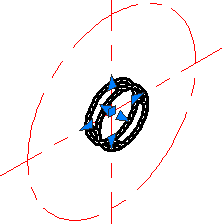
\includegraphics[scale=0.5]{duangaisolid1.png}}
\ffigbox{\caption{绘$\phi 24$圆柱体}\label{fig:duangaisolid2}}{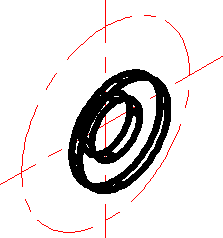
\includegraphics[scale=0.5]{duangaisolid2.png}}
\ffigbox{\caption{绘$\phi 42$圆柱体}\label{fig:duangaisolid3}}{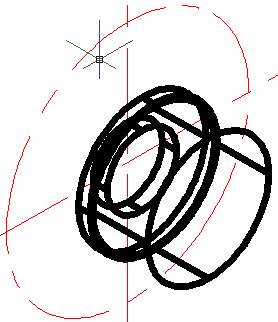
\includegraphics[scale=0.4]{duangaisolid3.png}}
\end{floatrow}
\end{figure}
\begin{lstlisting}
|命令: cylinder|
|指定底面的中心点或 [三点(3P)/两点(2P)/切点、切点、半径(T)/椭|
|圆(E)]:int于|
|指定底面半径或 [直径(D)]: 12|
|指定高度或 [两点(2P)/轴端点(A)]: 5|
\end{lstlisting}
以$\phi 24$圆柱体顶圆圆心为圆心绘制$\phi 44$圆柱体,结果如图\ref{fig:duangaisolid2}所示。
\begin{lstlisting}
|命令: cylinder|
|指定底面的中心点或 [三点(3P)/两点(2P)/切点、切点、半径(T)/椭|
|圆(E)]:int于|
|指定底面半径或 [直径(D)]$<$12.0000$>$: 22|
|指定高度或 [两点(2P)/轴端点(A)]$<$5.0000$>$: 4|
\end{lstlisting}
以$\phi 44$圆柱体顶圆圆心为圆心绘制$\phi 42$圆柱体,结果如图\ref{fig:duangaisolid3}所示。
\begin{lstlisting}
|命令: cylinder|
|指定底面的中心点或 [三点(3P)/两点(2P)/切点、切点、半径(T)/椭|
|圆(E)]:int于|
|指定底面半径或 [直径(D)]$<$22.0000$>$: 21|
|指定高度或 [两点(2P)/轴端点(A)]$<$4.0000$>$: 19|
\end{lstlisting}
以$\phi 42$圆柱体顶圆圆心为圆心绘制$\phi 62$圆柱体,结果如图\ref{fig:duangaisolid4}所示。
\begin{figure}[htbp]
\centering
\begin{floatrow}[3]
\ffigbox{\caption{绘$\phi 62$圆柱体}\label{fig:duangaisolid4}}{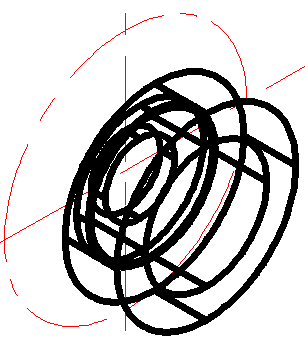
\includegraphics[scale=0.4]{duangaisolid4.png}}
\ffigbox{\caption{绘$\phi 9$圆柱体}\label{fig:duangaisolid5}}{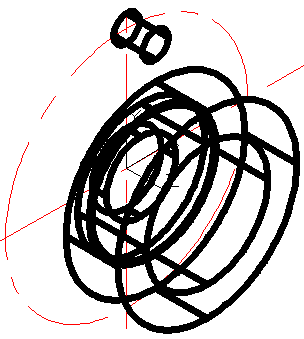
\includegraphics[scale=0.4]{duangaisolid5.png}}
\ffigbox{\caption{绘$\phi 104$圆柱体}\label{fig:duangaisolid6}}{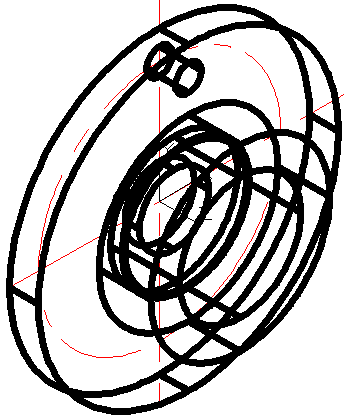
\includegraphics[scale=0.3]{duangaisolid6.png}}
\end{floatrow}
\end{figure}
\begin{lstlisting}
|命令: cylinder|
|指定底面的中心点或 [三点(3P)/两点(2P)/切点、切点、半径(T)/椭|
|圆(E)]:int于|
|指定底面半径或 [直径(D)]$<$21.0000$>$: 31|
|指定高度或 [两点(2P)/轴端点(A)]$<$19.0000$>$: -18|
\end{lstlisting}
以对称中心的交点为圆心绘制$\phi 9$圆柱体,结果如图\ref{fig:duangaisolid5}所示。
\begin{lstlisting}
|命令: cylinder|
|指定底面的中心点或 [三点(3P)/两点(2P)/切点、切点、半径(T)/椭|
|圆(E)]:int于|
|指定底面半径或 [直径(D)]$<$31.0000$>$: 9|
|指定高度或 [两点(2P)/轴端点(A)]$<$-18.0000$>$:10 |
\end{lstlisting}
以对称中心的交点为圆心绘制$\phi 104$圆柱体,结果如图\ref{fig:duangaisolid6}所示。
\begin{lstlisting}
|命令: cylinder|
|指定底面的中心点或 [三点(3P)/两点(2P)/切点、切点、半径(T)/椭|
|圆(E)]:int于|
|指定底面半径或 [直径(D)]$<$31.0000$>$: 52|
|指定高度或 [两点(2P)/轴端点(A)]$<$10.0000$>$: |
\end{lstlisting}
\item 合并实体。

将$\phi 104$圆柱体和$\phi 62$圆柱体合并为一个实体。
\begin{lstlisting}
|命令:UNION|
|选择对象: 找到 1 个|
|选择对象: 找到 1 个,总计 2 个|
|选择对象:|
\end{lstlisting}
\item 三维阵列$\phi 9$圆柱体。
\begin{lstlisting}
|命令: 3darray|
|选择对象: 找到 1 个|
|选择对象:|
|输入阵列类型 [矩形(R)/环形(P)]$<$矩形$>$:p|
|输入阵列中的项目数目: 6|
|指定要填充的角度 (+=逆时针, -=顺时针)$ <360>$:|
|旋转阵列对象? [是(Y)/否(N)] $<Y>$:|
|指定阵列的中心点:|
|指定旋转轴上的第二点:|
\end{lstlisting}
\item 用差集操作完成三维建模操作。
\begin{lstlisting}
|命令: subtract |
|选择要从中减去的实体、曲面和面域...|
|选择对象: 找到 1 个|
|选择对象:  选择要减去的实体、曲面和面域...|
|选择对象: 指定对角点: 找到 9 个|
|选择对象:|
\end{lstlisting}
\item 建立三维圆角。

建立三维圆角,既可使用二维【圆角】命令,也可以使用三维的【圆角边】命令。启动【圆角边】命令的方法有:
\begin{itemize}
\item 键盘输入FILLETEDGE\index{filletedge}。
\item 【修改】$\rightarrow$【实体编辑】$\rightarrow$【圆角边】。
\item 【实体编辑】$\triangleright$【圆角边】图标
\includegraphics[scale=0.6]{filletedge.png}。
\end{itemize} 

\begin{lstlisting}
|命令: FILLETEDGE|
|半径 = 1.0000|
|选择边或 [链(C)/环(L)/半径(R)]:|
|选择边或 [链(C)/环(L)/半径(R)]: r|
|输入圆角半径或 [表达式(E)]$<$1.0000$>$: 3|
|选择边或 [链(C)/环(L)/半径(R)]:|  
|选择边或 [链(C)/环(L)/半径(R)]:|
|选择边或 [链(C)/环(L)/半径(R)]:|
|已选定 3 个边用于圆角。|
|按 Enter 键接受圆角或 [半径(R)]:|
\end{lstlisting}
\item 设置视觉样式为真实,其结果如图\ref{fig:duangailititu}所示。
\item 将端盖模型保存为“调压阀端盖立体图.dwg”。
\end{procedure}


%%%%%%%%%%%%%%教案头%%%%%%%%%%%%%%%%%%%%%%%%%%%%%%%
\mode<article>{

\begin{longtable}{|m{20mm}|m{20mm}|m{20mm}|m{20mm}|m{20mm}|m{28mm}|}
\caption*{\huge 教案头}\\
\hline
\endfirsthead
\multicolumn{6}{l}{(续表)}\\
\hline
\endhead
\hline
\multicolumn{6}{l}{\itshape 接下一页表格.......}\\ [2ex]
\endfoot
\hline
\endlastfoot
\centering{授课单元}&\multicolumn{3}{m{60mm}|}{\centering 4.4z变换}&\centering{授课日期}&2014年06月4日 \\
\hline
\centering 授课地点 & \multicolumn{3}{m{60mm}|}{B6-204}&\centering 授课学时 & 2 \\
\hline
& \multicolumn{2}{m{40mm}|}{能力目标} & \multicolumn{2}{m{40mm}|}{知识目标}&素质目标 \\
\cline{2-6}
\centering 教学目标&\multicolumn{2}{m{40mm}|}{\begin{enumerate}
\item  能够进行离散信号的Z变换
\end{enumerate} }&\multicolumn{2}{m{40mm}|}{\begin{enumerate}
\item 了解Z变换的定义
\item 了解Z变换的求解方法
\item 了解Z变换的逆变换
\end{enumerate}} & {\qquad}\\
\hline
\centering 能力训练任务或案例 &\multicolumn{5}{m{108mm}|}{ }\\
\hline
\centering 教学重点 & \multicolumn{5}{m{108mm}|}{\begin{enumerate}
\item Z变换
\item Z变换的逆变换
\end{enumerate}}\\
\hline
\centering 教学难点与解决办法 &\multicolumn{5}{m{108mm}|}{\begin{enumerate}
\item 难点:Z变换的逆变换
\item 解决方法:实例讲解
\end{enumerate}}\\
\hline
\centering 德育内容 &\multicolumn{5}{m{108mm}|}{无}\\
\hline
 &教材 & \multicolumn{4}{m{88mm}|}{计算机控制原理与应用}\\
\cline{2-6}& 教学资源 &\multicolumn{4}{m{88mm}|}{PPT}\\
\cline{2-6}\centering 使用的教学材料& 主要教学仪器设备和工具等 &\multicolumn{4}{m{88mm}|}{投影机、MATLAB}\\
\cline{2-6}& 主要耗材 &\multicolumn{4}{m{88mm}|}{无}\\
\hline
\centering 教学模式 &\multicolumn{2}{m{40mm}|}{知识讲授}&\centering 教学手段 &\multicolumn{2}{m{48mm}|}{多媒体教学}\\
\hline
\centering 学生成果与过程考核方式 &\multicolumn{5}{m{108mm}|}{无}
\end{longtable}
\clearpage

%%%%%%%%%%%%%%%教学实施过程%%%%%%%%%%%%%%%%%%%%%%%%%%%%
\begin{landscape}

\begin{longtable}{|m{10mm}|m{50mm}|m{50mm}|m{50mm}|m{15mm}|}
\caption*{\huge 教学组织与实施}\\
\hline
\endfirsthead
\multicolumn{5}{l}{\small 接上页}\\
\hline
\multicolumn{1}{|c|}{步骤}&\multicolumn{1}{c|}{教学内容}&\multicolumn{1}{c|}{教师活动}&\multicolumn{1}{c|}{学生活动}&\multicolumn{1}{c|}{时间}\\
\hline
\endhead

\multicolumn{5}{r}{\small 接下页}\\
\endfoot
\hline
\endlastfoot
\multicolumn{1}{|c|}{步骤}&\multicolumn{1}{c|}{教学内容}&\multicolumn{1}{c|}{教师活动}&\multicolumn{1}{c|}{学生活动}&\multicolumn{1}{c|}{时间}\\\hline
讲解&\begin{enumerate}
\item Z变换的定义
\end{enumerate} &\begin{enumerate}
\item 讲解Z变换的定义
\end{enumerate} &\begin{enumerate}
\item 学生倾听并记录
\end{enumerate} &25\\\hline
讲解&\begin{enumerate}
\item Z变换的实例
\end{enumerate}
 &\begin{enumerate}
\item 讲解Z变换的例子
\end{enumerate} &\begin{enumerate}
\item 学生倾听并记录
\end{enumerate} &20 \\\hline
讲解&\begin{enumerate}
\item Z变换定理
\end{enumerate}
&\begin{enumerate}
\item 讲解Z变换定理
\end{enumerate} &\begin{enumerate}
\item 学生倾听并记录
\end{enumerate} &40 \\\hline

\centering 本次课总结(评价)&总结本课程内容 &进行知识总结 &学生倾听 &5 \\\hline
\centering 学生学习笔记或工单等检查情况&\multicolumn{4}{m{165mm}|}{\quad}\\\hline
\centering 课后作业&\multicolumn{4}{m{165mm}|}{2-28,2-29}\\\hline
\centering 教学体会&\multicolumn{4}{m{165mm}|}{\quad}\\
\end{longtable}

\end{landscape}
\clearpage
%%%%%%%%%%%%%%%%%%%%板书设计%%%%%%%%%%%%%%%%%%%%%%%%%%
\begin{center}
{\huge 板书设计}
\end{center}
}

 \begin{frame}{4.4Z变换} 
 \begin{block}{}
\[f^*(t)=\sum\limits_{k=0}^\infty f(kT)\delta(t-kT)\]
 \end{block}
 \begin{block}{拉氏变换得}
 \[F^*(s)=\sum\limits_{k=0}^\infty f(kT)e^{-kTs}\]
 \end{block}
 \end{frame}
 
 \begin{frame}
 \begin{block}{引入复变量Z}
\begin{eqnarray*}
z=e^{sT}\\
s=\frac{1}{T}\ln z
\end{eqnarray*}
\end{block}
\begin{block}{Z变换定义为}
\[F(z)=\sum\limits_{k=0}^\infty f(kT)z^{-k}\]
\end{block}
\end{frame}

\begin{frame}{Z变换定理}
\begin{block}{线性定理}
\[\pounds[af_1(t)+bf_2(t)]=aF_1(z)+bF_2(z)\]
\end{block}
\begin{block}{超前定理}
\[\pounds[f(t+nT)]=z^n\left[F(z)-\sum\limits_{q=0}^{n-1}f(qT)z^{-q}\right]\]
\end{block}

\end{frame}

\begin{frame}
\begin{block}{滞后定理}
\begin{equation*}
\pounds[f(t-nT)u(t-nT)]=z^{-n}F(z)
\end{equation*}
\end{block}
\begin{block}{有限和定理}
\begin{equation*}
\pounds\left[\sum\limits_{k=0}^nf(kT)\right]=\frac{F(z)}{1-z^{-1}}
\end{equation*}
\end{block}
\end{frame}

\begin{frame}
\begin{block}{阻尼定理}
\begin{eqnarray*}
\pounds[e^{at}f(t)]=F(e^{-aT}z)
\end{eqnarray*}
\end{block}
\begin{block}{复微分定理}
\begin{eqnarray*}
\pounds[tf(t)]=-Tz\frac{d}{dz}F(z)
\end{eqnarray*}
\end{block}
\end{frame}

\begin{frame}
\begin{block}{初值定理}
\begin{eqnarray*}
f(0)=\lim_{k\to 0}f(kT)=\lim_{z\to\infty}F(z)
\end{eqnarray*}
\end{block}
\begin{block}{终值定理}
\begin{eqnarray*}
f(\infty)=\lim_{k\to\infty}f(kT)=\lim_{z\to 1}(z-1)F(z)
\end{eqnarray*}
\end{block}
\end{frame}

\begin{frame}{Z逆变换}
\begin{block}{长除法}
先将$F(z)$展开为无穷幂级数,再逐项求$Z$逆变换,实际中只计算几项就够了。
\end{block}
\begin{block}{部分展开法}
若$F(z)$为有理函数,先将其展开,再逐项求$Z$逆变换。
\end{block}
\end{frame}
\begin{frame}{}
\begin{block}{留数法}
是一种公式法
\begin{eqnarray*}
f(kT)=\pounds^{-1}[F(z)]=\frac{1}{2\pi j}\oint_{\Gamma}F(z)z^{k-1}dz
\end{eqnarray*}
\end{block}
\begin{block}{由留数定理得}
\begin{eqnarray*}
f(kT)=f(k)=f_1+f_2+\cdots +f_n\\
\sum\limits_{k=1}^nRes[F(z)z^{k-1}]|_{z=p_i}
\end{eqnarray*}
\end{block}
\end{frame}
\begin{frame}
\begin{block}{当$p_i$为非重极点时}
\[Res[F(z)z^{k-1}]|_{z=p_i}=\lim_{z\to p_i}(z-p_i)F(z)z^{k-1}\]
则
\[f(kT)=\sum\limits_{i=1}^n\lim_{z\to p_i}(z-p_i)F(z)z^{k-1}\]
\end{block}
\end{frame}

\begin{frame}
\begin{block}{有m重极点时}
\begin{eqnarray*}
&&Res[F(z)z^{k-1}]=\\
&&\frac{1}{(m-1)!}\lim_{z\to p_j}\left\lbrace\frac{d^{m-1}}{dz^{m-1}}[(z-p_j)^mF(z)z^{k-1}]\right\rbrace\\
&&f(kT)=\sum\limits_{i=1}^{n-m}\lim_{z\to p_i}[(z-p_i)F(z)z^{k-1}+\\
&&\lim_{z\to p_j}\frac{1}{(m-1)!}\left\lbrace\frac{d^{m-1}}{dz^{m-1}}[(z-p_j)^mF(z)z^{k-1}]\right\rbrace
\end{eqnarray*}
\end{block}
\end{frame}
\begin{frame}
\begin{block}{计算法}
\begin{itemize}
\item Matlab法
\item 差分方程法
\end{itemize}
\end{block}
\end{frame}

\end{CJK}
\end{document}